\documentclass[12pt]{report}
\usepackage{amsmath}
\usepackage{amssymb}
\usepackage{graphicx}
\usepackage{physics}
\usepackage{tikz}
\usepackage{geometry}
\usepackage{algorithm}
\usepackage{algorithmic}
\usepackage[numbers]{natbib}
\bibliographystyle{plainnat}  % or another style like 'apsrev4-2'
\usepackage{hyperref}
\usepackage{bm}
\usepackage{xcolor}
\usepackage{listings}



\usepackage{listings} % Required for insertion of code
\usepackage{xcolor} % Required for custom colors

% Define custom colors
\definecolor{codegreen}{rgb}{0,0.6,0}
\definecolor{codegray}{rgb}{0.5,0.5,0.5}
\definecolor{codepurple}{rgb}{0.58,0,0.82}
\definecolor{backcolour}{rgb}{0.95,0.95,0.92}

% Setup the style for code listings
\lstdefinestyle{mystyle}{
    backgroundcolor=\color{backcolour},   
    commentstyle=\color{codegreen},
    keywordstyle=\color{magenta},
    numberstyle=\tiny\color{codegray},
    stringstyle=\color{codepurple},
    basicstyle=\ttfamily\footnotesize,
    breakatwhitespace=false,         
    breaklines=true,                 
    captionpos=b,                    
    keepspaces=true,                 
    numbers=left,                    
    numbersep=5pt,                  
    showspaces=false,                
    showstringspaces=false,
    showtabs=false,                  
    tabsize=2
}

% Activate the style
\lstset{style=mystyle}

\geometry{
    margin=1in,
    textwidth=6.5in,
    textheight=9in
}

\title{Patryk's Notes}
\author{Patryk Kozlowski}
\begin{document}

% Add detailed table of contents settings
\setcounter{tocdepth}{3}  % Show up to subsubsection level in TOC
\tableofcontents
\clearpage  % Start new page after TOC

\maketitle

% Rest of your document content
\chapter{$G_0W_0$ Derivations: 11/9}
\section{Deriving Hedin's equations}
\subsection{Time-Domain Definition of the Green's Function}
Start by considering the equation of motion for the field operators
\begin{equation}
  i\frac{\partial}{\partial t}\hat{\psi}(\mathbf{x}, t) = [\hat{\psi}(\mathbf{x}, t),\hat{H}_{elec}] = [\hat{\psi}(\mathbf{x}, t), \hat{H}_0 + \hat{H}_{int}] = [\hat{\psi}(\mathbf{x}, t), \hat{H}_0] + [\hat{\psi}(\mathbf{x}, t), \hat{H}_{int}] 
\end{equation}
For the non-interacting part, we have
\begin{align}
  [\hat{\psi}(\mathbf{x}, t), \hat{H}_0] &= [\hat{\psi}(\mathbf{x}, t), \int d\mathbf{x}' \hat{\psi}^\dagger(\mathbf{x}', t)\hat{h}^0(\mathbf{x}')\hat{\psi}(\mathbf{x}', t)] \\
  &= \int d\mathbf{x}' [\hat{\psi}(\mathbf{x}, t), \hat{\psi}^\dagger(\mathbf{x}', t)\hat{h}^0(\mathbf{x}')\hat{\psi}(\mathbf{x}', t)] \\
  &= \int d\mathbf{x}' \left( \underbrace{[\hat{\psi}(\mathbf{x}, t), \hat{\psi}^\dagger(\mathbf{x}', t)]}_{\delta(\mathbf{x}-\mathbf{x}')}\hat{h}^0(\mathbf{x}')\hat{\psi}(\mathbf{x}', t) + \hat{\psi}^\dagger(\mathbf{x}', t)\hat{h}^0(\mathbf{x}')\underbrace{[\hat{\psi}(\mathbf{x}, t), \hat{\psi}(\mathbf{x}', t)]}_{0} \right) \\
  &= h^0(\mathbf{x})\hat{\psi}(\mathbf{x}, t).
\end{align}
For the interacting part, we have
\begin{align}
 &[\hat{\psi}(\mathbf{x}, t), \hat{H}_{int}] = \frac{1}{2}\int d\mathbf{x}' d\mathbf{x}'' v(\mathbf{x},\mathbf{x}') [ \hat{\psi}(\mathbf{x}, t), \hat{\psi}^\dagger(\mathbf{x}', t)  \hat{\psi}^{\dagger}(\mathbf{x}'', t) \hat{\psi}(\mathbf{x}'', t) \hat{\psi}(\mathbf{x}', t) ] \\
&= \frac{1}{2}\int d\mathbf{x}' d\mathbf{x}'' v(\mathbf{x},\mathbf{x}') \left( \delta (\mathbf{x}-\mathbf{x}') \hat{\psi}^\dagger(\mathbf{x}'', t) \hat{\psi}(\mathbf{x}'', t) \hat{\psi}(\mathbf{x}', t) + \hat{\psi}^\dagger(\mathbf{x}', t) \delta (\mathbf{x}-\mathbf{x}'') \hat{\psi}(\mathbf{x}'', t) \hat{\psi}(\mathbf{x}', t) \right) \\
&= \int d\mathbf{x}' \hat{\psi}^\dagger(\mathbf{x}', t) v(\mathbf{x},\mathbf{x}') \hat{\psi}(\mathbf{x}', t) \hat{\psi}(\mathbf{x}, t)
\end{align}
so overall we have
\begin{equation}
  i\frac{\partial}{\partial t}\hat{\psi}(\mathbf{x}, t) = \left( \hat{h}^0(\mathbf{x}) + \int d\mathbf{x}' v(\mathbf{x},\mathbf{x}') \hat{\psi}^\dagger(\mathbf{x}', t) \hat{\psi}(\mathbf{x}', t) \right) \hat{\psi}(\mathbf{x}, t) 
\end{equation}
Now we can consider the equation of motion for the Green's function, defined as $G(\mathbf{x}t, \mathbf{x}'t') = -i \bra{N}\mathcal{T}\left(\hat{\psi}(\mathbf{x},t)\hat{\psi}^\dagger(\mathbf{x}',t')\right)\ket{N}$, where $\mathcal{T}$ is the time-ordering operator.
\begin{align}
  \frac{\partial}{\partial t}G(\mathbf{x}t, \mathbf{x}'t') &= -i \bra{N}\frac{\partial}{\partial t}\mathcal{T}\left(\hat{\psi}(\mathbf{x},t)\hat{\psi}^\dagger(\mathbf{x}',t')\right)\ket{N} \\
\end{align}
Now,
\begin{align}
  &\frac{\partial}{\partial t}\mathcal{T}\left(\hat{\psi}(\mathbf{x},t)\hat{\psi}^\dagger(\mathbf{x}',t')\right) = \frac{\partial}{\partial t}\left( \theta(t-t')\hat{\psi}(\mathbf{x},t)\hat{\psi}^\dagger(\mathbf{x}',t') - \theta(t'-t)\hat{\psi}^\dagger(\mathbf{x}',t')\hat{\psi}(\mathbf{x},t) \right) \\
  &= \underbrace{\frac{\partial \theta(t-t')}{\partial t}}_{\delta(t-t')}\hat{\psi}(\mathbf{x},t)\hat{\psi}^\dagger(\mathbf{x}',t') + \theta(t-t')\frac{\partial}{\partial t}\hat{\psi}(\mathbf{x},t)\hat{\psi}^\dagger(\mathbf{x}',t') - \underbrace{\frac{\partial \theta(t'-t)}{\partial t}}_{-\delta(t'-t)}\hat{\psi}^\dagger(\mathbf{x}',t')\hat{\psi}(\mathbf{x},t) - \theta(t'-t)\frac{\partial}{\partial t}\hat{\psi}^\dagger(\mathbf{x}',t')\hat{\psi}(\mathbf{x},t) \\
  &= \underbrace{\delta(t-t') {\acomm{\hat{\psi}(\mathbf{x},t)}{\hat{\psi}^\dagger(\mathbf{x}',t')}}}_{\delta(\mathbf{x}-\mathbf{x}') \delta(t-t')} + \mathcal{T}\left(\frac{\partial}{\partial t}\hat{\psi}(\mathbf{x},t)\hat{\psi}^\dagger(\mathbf{x}',t')\right) \\
\end{align}
So now consider plugging in the equation of motion for $\hat{\psi}(\mathbf{x},t)$ into the above expression
\begin{align}
  &\mathcal{T}\left(\frac{\partial}{\partial t}\hat{\psi}(\mathbf{x},t)\hat{\psi}^\dagger(\mathbf{x}',t')\right) = \mathcal{T}\left(-i \left( \hat{h}^0(\mathbf{x}) + \int d\mathbf{x}'' v(\mathbf{x},\mathbf{x}'') \hat{\psi}^\dagger(\mathbf{x}'',t) \hat{\psi}(\mathbf{x}'',t) \right) \hat{\psi}(\mathbf{x},t)\hat{\psi}^\dagger(\mathbf{x}',t')\right) \\
  &=  -i \hat{h}^0(\mathbf{x}) \mathcal{T}\left(\hat{\psi}(\mathbf{x},t)\hat{\psi}^\dagger(\mathbf{x}',t')\right) - i \int d\mathbf{x}'' v(\mathbf{x},\mathbf{x}'') \mathcal{T}\left(\hat{\psi}(\mathbf{x},t)\hat{\psi}^\dagger(\mathbf{x}'',t) \hat{\psi}(\mathbf{x}'',t) \hat{\psi}^\dagger(\mathbf{x}',t')\right)
\end{align}
So we have
\begin{align}
  \left[ i \frac{\partial}{\partial t} - \hat{h}^0(\mathbf{x}) \right] G(\mathbf{x}t, \mathbf{x}'t') = \delta(\mathbf{x}-\mathbf{x}') \delta(t-t') - i \int d\mathbf{x}'' v(\mathbf{x},\mathbf{x}'') \underbrace{G_2(\mathbf{x}t, \mathbf{x}''t, \mathbf{x}'t^+ , \mathbf{x}'t')}_{\bra{N}\mathcal{T}\left(\hat{\psi}(\mathbf{x},t)\hat{\psi}(\mathbf{x}'',t)\hat{\psi}^\dagger(\mathbf{x}'',t')\hat{\psi}^\dagger(\mathbf{x}',t')\right)\ket{N}}
\end{align}
and we notice that in order to compute the single-particle Green's function, we need to know the two-particle Green's function, which needs the three-particle Green's function, and so on. So to simplify we introduce a nonlocal, time-dependent self-energy $\Sigma(\mathbf{x}t, \mathbf{x}'t')$ that satisfies
\begin{align}
  - i \int d\mathbf{x}'' v(\mathbf{x}, \mathbf{x}'') G_2(\mathbf{x}t, \mathbf{x}''t, \mathbf{x}'t^+ , \mathbf{x}'t') \equiv \int dt'' \int d\mathbf{x}'' \overline{\Sigma}(\mathbf{x} t , \mathbf{x}'' t'' ) G(\mathbf{x}''t'', \mathbf{x}'t')
\end{align}
and further define $\Sigma = \overline{\Sigma} - v_H$ with
\begin{align}
  v_H(\mathbf{x},t) = \int d\mathbf{x}' v(\mathbf{x}, \mathbf{x}') \underbrace{\bra{N} \hat{\psi}^\dagger(\mathbf{x}') \hat{\psi}(\mathbf{x}') \ket{N}}_{-\frac{1}{i}G(\mathbf{x}'t, \mathbf{x}'t)} = i \int d\mathbf{x}' v(\mathbf{x}, \mathbf{x}') G(\mathbf{x}'t, \mathbf{x}'t)
  \label{eq:hartree}
\end{align}
and we can rewrite the equation of motion as
\begin{align}
  \left[ i \frac{\partial}{\partial t} - \hat{h}^0(\mathbf{x}) - v_H(\mathbf{x},t) \right] G(\mathbf{x}t, \mathbf{x}'t') = \delta(\mathbf{x}-\mathbf{x}') \delta(t-t') + \int dt'' \int d\mathbf{x}'' \Sigma(\mathbf{x}t, \mathbf{x}''t'') G(\mathbf{x}''t'', \mathbf{x}'t')
  \label{eq:eom_green}
\end{align}
Now consider defining the $G_0$ of the non-interacting system
\begin{align}
    \left[ i \frac{\partial}{\partial t} - \hat{h}^0(\mathbf{x}) - v_H(\mathbf{x},t) \right] G_0(\mathbf{x}t, \mathbf{x}'t') = \delta(\mathbf{x}-\mathbf{x}') \delta(t-t')
    \label{eq:eom_green_0}
\end{align}
So we can write equations \ref{eq:eom_green} and \ref{eq:eom_green_0} symbolically as
\begin{align}
  \hat{O} G &= \delta + \Sigma G \quad \text{and} \quad \hat{O} G_0 = \delta \\
  &\implies G_0 = \hat{O}^{-1} \implies G = G_0 + G_0 \Sigma G \\
  &\implies G(1,2) = G_0(1,2) + \int d3 d4 G_0(1,3) \Sigma(3,4) G(4,2)
\end{align}
where we use the space-time notation $1 = (\mathbf{x}_1,t_1)$ etc.

\subsection{Hedin's Equations}
Schwinger chose to introduce a potential $\varphi$ that we will later set to zero, in order to rewrite the two-particle Green's function as
\begin{equation}
  G_2(1,3,2,3^+) = G(1,2) \, G(3,3^+) - \frac{\delta G(1,2)}{\delta \varphi(3)},
  \label{eq:schwinger}
\end{equation}
So
\begin{align}
  \bar{\Sigma}(1,2) &= -i \int d(3) \; v(1,3)\, G_2(1,3,2,3^+) \\
  &= -i \int d(3)\, v(1,3) \left[ G(1,2)\, G(3,3^+) - \frac{\delta G(1,2)}{\delta \varphi(3)} \right] \\
  &= -i\, G(1,2) \underbrace{\int d(3)\, v(1,3)\, G(3,3^+)}_{-i v_H(1)} + i \int d(3)\, v(1,3)\, \frac{\delta G(1,2)}{\delta \varphi(3)}.
  \label{eq:sigma_intermediate}
\end{align}
Now because $\delta G = -G  \left( \delta G^{-1} \right) G$ we can write the identity
\begin{equation}
  \frac{\delta G(1,2)}{\delta \varphi(3)} = - \int d(4)d(5) \; G(1,4) \, \frac{\delta G^{-1}(4,5)}{\delta \varphi(3)} \, G(5,2).
  \label{eq:deltaG}
\end{equation}
So the second term in Eq.~\eqref{eq:sigma_intermediate} gives
\begin{align}
  i\int d(3)\; v(1,3)\, \frac{\delta G(1,2)}{\delta \varphi(3)}
  &= -i \int d(3) \, v(1,3) \int d(4)d(5) \; G(1,4) \, \frac{\delta G^{-1}(4,5)}{\delta \varphi(3)} \, G(5,2) \nonumber \\
  &= -i \int d(3,4,5) \; v(1,3)\, G(1,4)\, \frac{\delta G^{-1}(4,5)}{\delta \varphi(3)}\, G(5,2).
  \label{eq:second_term}
\end{align}
Now we can get rid of a \(G(1,2)\) dependence by multiplying with \(G^{-1}\), yielding
\begin{equation}
  \overline{\Sigma}(1,2) = -\delta(1,2)\,v_H(1) -i\int d(3,4)\; v(1,3)\, G(1,4)\, \frac{\delta G^{-1}(4,2)}{\delta \varphi(3)}.
  \label{eq:sigma_final}
\end{equation}
Introduce $V(1) = \varphi(1) + v_H(1)$ as the total potential that electrons experience. Consider
\begin{equation}
  \frac{\delta G^{-1}(1,2)}{\delta \varphi(3)} \equiv \underbrace{\frac{\delta G^{-1}(1,2)}{\delta V(5)}}_{-\Gamma(1,2,5)} \underbrace{\frac{\delta V(5)}{\delta \varphi(3)}}_{\varepsilon^{-1}(5,3)}.
  \label{eq:deltaG_V}
\end{equation}
So
\begin{align}
  \overline{\Sigma}(1,2) = -\delta(1,2)\,v_H(1) +i\int d(5) \underbrace{\int d(3) v(1,3)\, \varepsilon^{-1}(3,5)}_{W(1,5 )}\, \int d(4) G(1,4)\, \Gamma(4,5,2).
  \label{eq:sigma_final_2}
\end{align}
and if we further make the GW approximation where $\Gamma(4,5,2) \approx \delta(4,5)\delta(2,5)$ we get
\begin{equation}
  \overline{\Sigma}(1,2)  = -\delta(1,2)\,v_H(1) + iW(1,2) G(1,2)
  \label{eq:sigma_final_3}
\end{equation}
and if we just care about the exchange-correlation part, we can define
\begin{align}
   {\Sigma}_{xc}(1,2) = \overline{\Sigma}(1,2) + \delta(1,2)\,v_H(1) = i W(1,2) G(1,2) \implies \Sigma_{xc}(\tau) = i W(\tau) G(\tau)
  \label{eq:sigma_xc}
\end{align}
where $\tau = t_1 - t_2$. Define $G(\tau) = \int \frac{d\omega'}{2\pi} e^{-i\omega'\tau} G(\omega')$ and $W(\tau) = \int \frac{d\omega''}{2\pi} e^{-i\omega''\tau} W(\omega'')$ to get
\begin{equation}
  \Sigma_{xc}(\tau) = i \int \frac{d\omega'}{2\pi} \int \frac{d\omega''}{2\pi} e^{-i(\omega'+\omega'')\tau} G(\omega') W(\omega'')
  \label{eq:sigma_xc_freq}
\end{equation}
Taking the inverse Fourier transform of $\Sigma_{xc}(\tau)$ we get
\begin{equation}
  \Sigma_{xc}(\omega) = \int \frac{d\tau}{2\pi} e^{i\omega\tau} \Sigma_{xc}(\tau) = i \int \frac{d\omega'}{2\pi} \int \frac{d\omega''}{2\pi} G(\omega') W(\omega'') \underbrace{\int d\tau  e^{i(\omega -\omega'-\omega'')\tau}}_{2\pi \delta(\omega -\omega'-\omega'')} = i \int \frac{d\omega'}{2\pi} G(\omega') W(\omega-\omega')
  \label{eq:sigma_xc_inv_freq}
\end{equation}
Now in $G_0W_0$ one applies the Cauchy residue theorem to solve this convolution integral, yielding
the known form.





\section{Final expressions}
\subsection{Fully analytic}
I follow the notation of Tianyu's paper throughout this section \cite{Zhu2020-nt}.
    We want to solve for the self-energy whose form along the real axis is:
    \begin{equation}
    \Sigma\left(\mathbf{r}, \mathbf{r}^{\prime}, \omega\right)=\frac{i}{2 \pi} \int_{-\infty}^{\infty} e^{i\omega ^{\prime}\eta }d \omega^{\prime} G_{0}\left(\mathbf{r}, \mathbf{r}^{\prime}, \omega+\omega^{\prime}\right) W_{0}\left(\mathbf{r}, \mathbf{r}^{\prime}, \omega^{\prime}\right)
    \end{equation}
    In the molecular brutal basis, the self energy is given as:
    \begin{equation}
        \Sigma_{n n^\prime}(\mathbf{k}, \omega) = \iint d \mathbf{r} d \mathbf{r}^\prime \psi_{n\mathbf{k}}^{*}(\mathbf{r}) \Sigma(\mathbf{r}, \mathbf{r}^\prime, \omega) \psi_{n^\prime\mathbf{k}}(\mathbf{r}^\prime)
    \end{equation}
    Also, recall that the Lehmann representation of the noninteracting Green's function is:
    \begin{equation}
        G_0\left(\mathbf{r}, \mathbf{r}^{\prime}, \omega\right)=\sum_{o \mathbf{q} } \frac{\psi_{o \mathbf{q}}(\mathbf{r}) \psi_{o \mathbf{q}}^{*}\left(\mathbf{r}^{\prime}\right)}{\omega-\epsilon_{o \mathbf{q}}+i \eta \operatorname{sgn}\left(\epsilon_{o \mathbf{q}}-\mu\right)}
    \end{equation}
    Now plugging both of these back into the original expression, we find:


    \begin{align}
        \Sigma_{n n^\prime}(\mathbf{k}, \omega) &= \frac{i}{2 \pi} \sum_{o \mathbf{q}} \int_{-\infty}^{\infty} d \omega^{\prime} \frac{e^{i\omega ^{\prime}\eta }}{\omega + \omega^{\prime} - \epsilon_{o \mathbf{q}} + i \eta \operatorname{sgn}\left(\epsilon_{o \mathbf{q}}-\mu\right)} \nonumber \\
        &\quad \times \iint d \mathbf{r} d \mathbf{r}^\prime \psi_{n\mathbf{k}}^{*}(\mathbf{r}) \psi_{o \mathbf{q}}(\mathbf{r}) W_0(\mathbf{r}, \mathbf{r}^\prime, \omega^{\prime}) \psi_{o \mathbf{q}}^{*}\left(\mathbf{r}^{\prime}\right) \psi_{n^\prime\mathbf{k}}(\mathbf{r}^\prime)\\
        &= \frac{i}{2 \pi} \sum_{o \mathbf{q}} \int_{-\infty}^{\infty} d \omega^{\prime} \frac{e^{i\omega ^{\prime}\eta }}{\omega + \omega^{\prime} - \epsilon_{o \mathbf{k}-\mathbf{q}} + i \eta \operatorname{sgn}\left(\epsilon_{o \mathbf{k}-\mathbf{q}}-\mu\right)} (n_{\mathbf{k}}o_{\mathbf{k-q}}|W_0|o_{\mathbf{k-q}}n^\prime_{\mathbf{k}})
    \end{align}
    Where we have used the fact that the momentum index $\mathbf{q}$ is the same as $\mathbf{k}-\mathbf{q}$, given that we are looping over both $\mathbf{k}$ and $\mathbf{q}$ anyways.


    So the Green's function will bring poles at \(\omega' = \epsilon_{0 \mathbf{k-q}} - \omega+ i\eta\operatorname{sgn}(\mu - \epsilon_{0 \mathbf{k-q}})\).
    Now, we know that the screened Coulomb interaction has the expansion in terms of the bare Coulomb potential \(v\) and the density response function \(\chi_0\) as \(W_0 = v + v\chi_0 v + v\chi_0 v\chi_0 v + \cdots = v\left(1 + \chi_0 v + \chi_0 v \chi_0 v + \cdots\right) = v\left(1 - \chi_0 v\right)^{-1}\), where we recognize the dielectric function as \(\epsilon_0 = 1 - \chi_0 v\) so we can express the screened Coulomb interaction as
    \begin{equation}
    W_0(\mathbf{r}, \mathbf{r}^{\prime}, \omega) = \frac{v(\mathbf{r}, \mathbf{r}^{\prime})}{1 - \left(\chi_0v\right)(\mathbf{r}, \mathbf{r}^{\prime}, \omega)}
    \end{equation}
    recalling that the bare Coulomb interaction should be independent of frequency. A discussion of how to compute the screened Coulomb interaction can be found in this old work \cite{Onida2002-pw}. To simplify notation let us define a polarizability $\boldsymbol{\Pi}\left(\mathbf{r}, \mathbf{r}^{\prime}, \omega\right) = \left(\chi_0 v\right)(\mathbf{r}, \mathbf{r}^{\prime}, \omega)$, so that we can rewrite the screened Coulomb interaction as:
\begin{align}
    (n_{\mathbf{k}}o_{\mathbf{k-q}}|W_0|o_{\mathbf{k-q}}n^\prime_{\mathbf{k}}) = \iint d \mathbf{r} d \mathbf{r}^\prime \psi_{n\mathbf{k}}^{*}(\mathbf{r}) \psi_{o \mathbf{q}}(\mathbf{r}) W_0(\omega ) \psi_{o \mathbf{q}}^{*}\left(\mathbf{r}^{\prime}\right) \psi_{n^\prime\mathbf{k}}(\mathbf{r}^\prime)
\end{align}
At this point, we recognize the decomposition of the ERIs with the Cholesky vectors as:
\begin{equation}
    (p_{\mathbf{k}_p} q_{\mathbf{k}_q} |\frac{1}{|\mathbf{r}-\mathbf{r}^\prime|} |r_{\mathbf{k}_r} s_{\mathbf{k}_s}) = \sum_{PQ} v_{P{\mathbf{q}}}^{p\mathbf{k_p}q\mathbf{k_q}} v_{Q{(\mathbf{-q})}}^{r\mathbf{k_r}s\mathbf{k_s}}
\end{equation}
so each Cholesky brings a factor of $\mathbf{J}^{\frac{1}{2}}$. Each Cholesky is defined as:
\begin{equation}
    v_{P{\mathbf{q}}}^{p\mathbf{k_p}q\mathbf{k_q}} = \sum_{R} \mathbf{J}_{RP}^{-\frac{1}{2}}(\mathbf{q}) \left(R \mathbf{q} \mid p \mathbf{k}_p q \mathbf{k}_q\right)
\end{equation}
where
\begin{equation}
\begin{aligned}
\mathbf{J}_{PQ}(\mathbf{k}) & =\iint d \mathbf{r} d \mathbf{r}^{\prime} \phi_{P(-\mathbf{k})}(\mathbf{r}) \frac{1}{\left|\mathbf{r}-\mathbf{r}^{\prime}\right|} \phi_{Q \mathbf{k}}\left(\mathbf{r}^{\prime}\right) \\
\left(Q \mathbf{k}_{r s} \mid r \mathbf{k}_r s \mathbf{k}_s\right) & =\iint d \mathbf{r} d \mathbf{r}^{\prime} \phi_{Q \mathbf{k}_{r s}}(\mathbf{r}) \frac{1}{\left|\mathbf{r}-\mathbf{r}^{\prime}\right|} \phi_{r \mathbf{k}_r}^*\left(\mathbf{r}^{\prime}\right) \phi_{s \mathbf{k}_s}\left(\mathbf{r}^{\prime}\right)
\end{aligned}
\end{equation}
So the simplest thing now will be to derive an expression for the columb interaction in terms of an auxiliary basis:
\begin{equation}
W_{0, PQ}(\omega)=\left[\mathbf{J}(\mathbf{I}-\mathbf{\Pi}(\mathbf{q}, \omega))^{-1}\right]_{PQ}
\end{equation}
and then we need to contract with the Choleskies to get the matrix element:
\begin{equation}
    (n_{\mathbf{k}}o_{\mathbf{k-q}}|W_0|o_{\mathbf{k-q}}n^\prime_{\mathbf{k}}) =\sum_{PQ} v_{P}^{nm}\left[\mathbf{I}-\mathbf{\Pi}\left(\mathbf{q}, \omega\right)\right]_{PQ}^{-1} v_{Q}^{mn^{\prime}}
\end{equation}

So in our quest to find poles of $W_0$, we are really just looking for poles of the $\chi_0$. $\chi_0$ is given by:
\begin{equation}
\chi_{0}\left(\mathbf{r}, \mathbf{r}^{\prime}, \omega\right)=\sum_{r\mathbf{k} s \mathbf{k}^{\prime}}\left(f_{r \mathbf{k}}-f_{s \mathbf{k}^{\prime}}\right) \frac{\psi_{r \mathbf{k}}(\mathbf{r}) \psi_{r \mathbf{k}}^{*}\left(\mathbf{r}^{\prime}\right) \psi_{s \mathbf{k}^{\prime}}\left(\mathbf{r}^{\prime}\right) \psi_{s \mathbf{k}^{\prime}}^{*}(\mathbf{r})}{\omega-\left(\epsilon_{r \mathbf{k}}-\epsilon_{s \mathbf{k}^{\prime}}\right)+i \eta \operatorname{sgn}\left(\epsilon_{r \mathbf{k}}-\epsilon_{s \mathbf{k}^{\prime} } - \mu\right)}
\end{equation}
where the occupations of the KS states \(r\mathbf{k}(s\mathbf{k}^{\prime})\) with energies \(\epsilon_{r\mathbf{k}}(\epsilon_{s\mathbf{k}^{\prime}})\) are given by the Fermi-Dirac distribution \(f_{r\mathbf{k}}(f_{s\mathbf{k}^{\prime}})\), which is just a step function at zero temperature. Notice that the occupation factor will always be 0 unless \(rs\) form an occupied-virtual pair. So we can separate the density response into two terms, one where \(\delta_{ri}\) and \(\delta_{sa}\) and the other with \(\delta_{ra}\) and \(\delta_{si}\), where \(i\) and \(a\) are occupied and virtual indices, respectively. This allows us to now combine with the bare Coulomb potential in order to form the polarizability \(\Pi\equiv \chi_0v\) as:
\begin{equation}
\Pi\left(\mathbf{r}, \mathbf{r}^{\prime}, \omega\right)=\sum_{i\mathbf{k}a\mathbf{k}^{\prime}}\frac{\psi_{i\mathbf{k}}(\mathbf{r}) \psi_{i\mathbf{k}}^{*}\left(\mathbf{r}^{\prime}\right)\frac{1}{|\mathbf{r}-\mathbf{r}^\prime|} \psi_{a\mathbf{k}^{\prime}}\left(\mathbf{r}^{\prime}\right) \psi_{a\mathbf{k}^{\prime}}^{*}(\mathbf{r})}{\omega+\left(\Omega_{i\mathbf{k}a\mathbf{k}^{\prime}}\right)-i\eta } - \sum_{a\mathbf{k}i\mathbf{k}^{\prime}}\frac{\psi_{a\mathbf{k}}(\mathbf{r}) \psi_{a\mathbf{k}}^{*}\left(\mathbf{r}^{\prime}\right) \frac{1}{|\mathbf{r}-\mathbf{r}^\prime|}\psi_{i\mathbf{k}^{\prime}}\left(\mathbf{r}^{\prime}\right) \psi_{i\mathbf{k}^{\prime}}^{*}(\mathbf{r})}{\omega-\left(\Omega_{i\mathbf{k}a\mathbf{k}^{\prime}}\right)+i\eta },
\end{equation}
where we define the KS eigenvalue differences as \(\Omega_{i\mathbf{k}a\mathbf{k}^{\prime}} = \epsilon_{a\mathbf{k}} - \epsilon_{i\mathbf{k}^{\prime}}\), which will eventually become the excitation energies from RPA. So sandwiching this operator in between the molecular or brutal bases gives:
\begin{equation}
    \bra{n\mathbf{k}} \Pi (\omega) \ket{n^\prime\mathbf{k}} = \sum_{iajb \mathbf{k} \mathbf{k}^{\prime}} \frac{(ia\mid jb)}{(\omega + \Omega ^{\mu}_{\mathbf{k}})-i\eta} - \sum_{aibj \mathbf{k} \mathbf{k}^{\prime}} \frac{(ai\mid bj)}{(\omega - \Omega ^{\mu}_{\mathbf{k}})+i\eta}
\end{equation}
\emph{So we see that we can get the poles of the screened Coulomb interaction by the poles of the polarizability, which are \(\omega = \Omega ^{\mu}_{\mathbf{k}} - i\eta\) and \(\omega = \Omega ^{\mu}_{\mathbf{k}} + i\eta\), suggesting that they are in the upper complex plane for excitations and vice versa for deexcitations.} See the figure \ref{fig:contour} for a picture. For a more comprehensive picture, this should be juxtaposed with the figure from Tianyu's paper for CD. In the literature, they talk about approximating the dielectric function by a multiple one or a single pole approximation, so which one would I want to implement? This suggests that the notation in the \(G_0W_0\) literature is confusing because they always say that to solve for the \(\chi_0\) in the RPA, but if we are actually dealing with \(\chi_0\), which is the Kohn-Sham density response function, then we don't use the RPA, where the density response function is solved for using a Dyson-like equation \cite{Sander2015-xq}:
    \begin{figure}[h]
    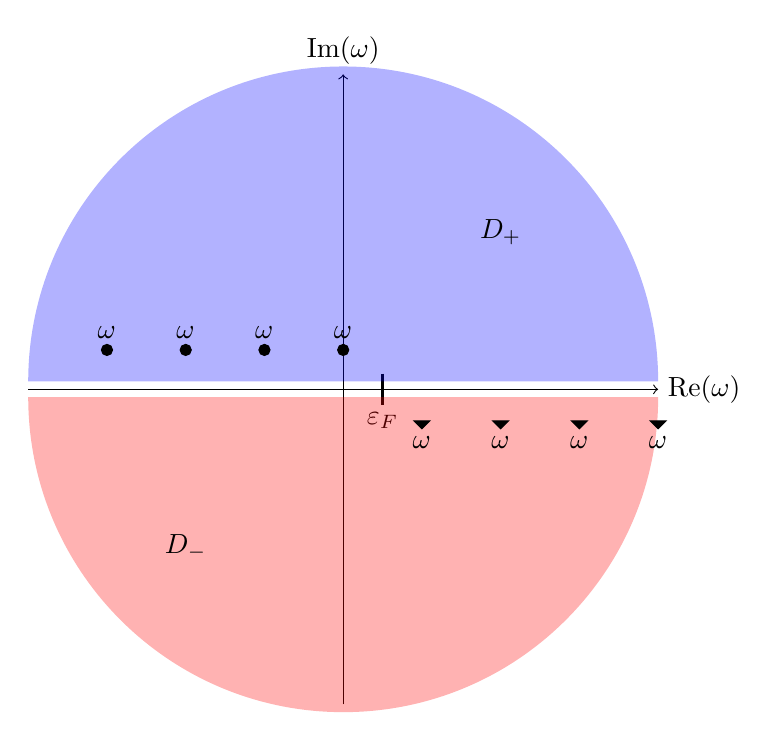
\begin{tikzpicture}
    % Draw the axes
    \draw[->] (-4, 0) -- (4, 0) node[right] {Re($\omega$)};
    \draw[->] (0, -4) -- (0, 4) node[above] {Im($\omega$)};
    
    % Draw the positive real axis label and tick mark for \varepsilon_{F}
    \draw[thick] (0.5, 0.2) -- (0.5, -0.2);
    \node at (0.5, -0.4) {$\varepsilon_{F}$};


    % Draw the semicircle contours
    % fill in its under side
    \fill[blue, opacity=0.3] (4, 0.1) arc[start angle=0, end angle=180, radius=4];
    \fill[red, opacity=0.3] (4, -0.1) arc[start angle=0, end angle=-180, radius=4];
    
    % Draw the poles above the real axis
    \foreach \x in {-3,-2,-1,0} {
        \draw[fill=black] (\x, 0.5) circle (2pt);
    }
    \node at (-3, 0.7) {$\omega_{}$};
    \node at (-2, 0.7) {$\omega_{}$};
    \node at (-1, 0.7) {$\omega_{}$};
    \node at (0, 0.7) {$\omega_{}$};    

    % Draw the poles below the real axis
    \foreach \x in {1,2,3,4} {
        \draw[fill=black] (\x, -0.5) -- ++(0.1, 0.1) -- ++(-0.2, 0) -- cycle;
    }
    \node at (1, -0.7) {$\omega_{}$};
    \node at (2, -0.7) {$\omega_{}$};
    \node at (3, -0.7) {$\omega_{}$};
    \node at (4, -0.7) {$\omega_{}$};

    
    % Label the contours
    \node at (2, 2) {$D_+$};
    \node at (-2, -2) {$D_-$};
    \end{tikzpicture}
    \caption{Contour for the complex frequency integral. The poles are denoted by the various $\omega$. The Fermi energy is denoted by $\varepsilon_F$. The integration contour $D_+$ is the semicircle in the upper complex plane, while $D_-$ is the semicircle in the lower complex plane.}
    \label{fig:contour}
    \end{figure}
\begin{equation}\label{eq:dyson}
    \chi^{\lambda}\left(\mathbf{r}, \mathbf{r}^{\prime}, i \omega\right) = \chi^{0}\left(\mathbf{r}, \mathbf{r}^{\prime}, i \omega\right) 
    + \int d \mathbf{r}_{1} d \mathbf{r}_{2} \chi^{0}\left(\mathbf{r}, \mathbf{r}_{1}, i \omega\right)\left[\frac{\lambda}{\left|\mathbf{r}_{1}-\mathbf{r}_{2}\right|}+f_{\mathrm{xc}}^{\lambda}\left(\mathbf{r}_{1}, \mathbf{r}_{2}, i \omega\right)\right] \chi^{\lambda}\left(\mathbf{r}_{2}, \mathbf{r}^{\prime}, \omega\right)
\end{equation}
where the parameter $\lambda$ controls the amount of interaction in the system, ranging from $\lambda = 0$ for the KS reference system to $\lambda = 1$ for the fully interacting system. The $f_{\mathrm{xc}}^{\lambda}$ is the exchange-correlation kernel, which is set to zero for the RPA. But we will proceed with an RPA calculation anyways in order to solve for the excitation energies and their corresponding eigenvectors. So it makes sense that the numerator of the expression for the screened Coulomb interaction should be given a construction of the ERIs with the excitation factors in a transition density defined as:
\begin{equation}
    w_{pq}^{\mu} = \sum_{ia} (pq|ia) \left(X_{ia}^{\mu} + Y_{ai}^{\mu}\right)
\end{equation}
where we have defined the excitation and de-excitation vectors at the excitation index $\mu$ as $X_{ia}^{\mu}$ and $Y_{ai}^{\mu}$, respectively.
I am not sure how to connect this with the known expression $v\epsilon ^{-1}$; I see the similarities given that we are contracting an ERI with what we get from the RPA calculation that is connected to the polarizability, but can't connect exactly.
We want to figure out how this matches with my previous $O(N^6)$ expression, which was
\begin{equation}
    \Sigma_{pp}^{\text{corr}}(\omega) = \sum_{\mu }^{\text{RPA}}\left(\sum_{i}^{\text{occupied}} \frac{w_{pi}^{\mu }w_{ip}^{\mu }}{\omega -(\epsilon _{i}-\Omega  _{\mu })}+ \sum_{a}^{\text{virtual}} \frac{w_{pa}^{\mu }w_{ap}^{\mu }}{\omega -(\epsilon _{a}+\Omega  _{\mu })}\right)
\end{equation}
for the molecular case. Today I want us to dissect how this equation came about, so that I can understand for my k-point version.
% The expression I get adapted for k-points from GPT is:
% \begin{equation}
% \Sigma_{n n^\prime}^{\text {corr }}(\mathbf{k}, \omega)=\sum_{\mathbf{q}} \sum_\mu^{\text {RPA }}\left(\sum_i^{\text {occupied }} \frac{w_{n i}^\mu(\mathbf{k}, \mathbf{q}) w_{i n^\prime}^\mu(\mathbf{k}-\mathbf{q}, \mathbf{q})}{\omega-\left(\epsilon_{i, \mathbf{k}-\mathbf{q}}-\Omega_{\mu, \mathbf{q}}\right)}+\sum_a^{\text {virtual }} \frac{w_{n a}^\mu(\mathbf{k}, \mathbf{q}) w_{a n^\prime}^\mu(\mathbf{k}-\mathbf{q}, \mathbf{q})}{\omega-\left(\epsilon_{a, \mathbf{k}-\mathbf{q}}+\Omega_{\mu, \mathbf{q}}\right)}\right)
% \end{equation}

\subsection{Analytic continuation}
\label{sec:analytic_continuation}
We start with the original form for the self-energy along the real axis:
\begin{equation}
\Sigma\left(\mathbf{r}, \mathbf{r}^{\prime}, \omega\right)=\frac{i}{2 \pi} \int_{-\infty}^{\infty} d \omega^{\prime} e^{i \omega^{\prime} \eta} G_{0}\left(\mathbf{r}, \mathbf{r}^{\prime}, \omega+\omega^{\prime}\right) W_{0}\left(\mathbf{r}, \mathbf{r}^{\prime}, \omega^{\prime}\right)
\end{equation}
But to avoid the poles, we need to evaluate along the imaginary axis, so the problem becomes:
\begin{equation*}
\Sigma\left(\mathbf{r}, \mathbf{r}^{\prime}, i \omega\right)=-\frac{1}{2 \pi} \int_{-\infty}^{\infty} d \omega^{\prime} G_{0}\left(\mathbf{r}, \mathbf{r}^{\prime}, i \omega+i \omega^{\prime}\right) W_{0}\left(\mathbf{r}, \mathbf{r}^{\prime}, i \omega^{\prime}\right) 
\end{equation*}
We are interested in evaluating the matrix elements of this operator in the molecular orbital basis. Note that both molecular orbitals must have the same crystal momentum in order for it to be conserved in this process. We also apply the identity operator:
\begin{equation}
\bra{n\mathbf{k}} \Sigma (i \omega) \ket{n^\prime\mathbf{k}} = -\frac{1}{2 \pi} \sum_{m\mathbf{k}^\prime}\int_{-\infty}^{\infty} d \omega^{\prime} \bra{n\mathbf{k}} G_0(i \omega + i \omega^{\prime}) \ket{m\mathbf{k^\prime}}\bra{m\mathbf{k^\prime}}W_0(i \omega^{\prime}) \ket{n^\prime\mathbf{k}}
\end{equation}
The noninteracting Green's function has the form:
\begin{equation*}
G_{0}\left(\mathbf{r}, \mathbf{r}^{\prime}, i \omega\right)=\sum_{m \mathbf{k}_{m}} \frac{\psi_{m \mathbf{k}_{m}}(\mathbf{r}) \psi_{m \mathbf{k}_{m}}^{*}\left(\mathbf{r^\prime}\right)}{i \omega+\epsilon_{F}-\epsilon_{m \mathbf{k}_{m}}} \implies G_{0}\left(\mathbf{k} - \mathbf{q}, i \omega + i \omega^{\prime}\right) = \sum_{m \mathbf{k}-\mathbf{q}} \frac{\psi_{m \mathbf{k}-\mathbf{q}} \psi_{m \mathbf{k}-\mathbf{q}}^{*}}{i \left(\omega + \omega^{\prime}\right) + \epsilon_{F} - \epsilon_{m \mathbf{k}-\mathbf{q}}}
\end{equation*}
so that the above equation simplifies to:
\begin{equation}
\boldsymbol{\Sigma}_{n n^{\prime}}(\mathbf{k}, i \omega) = -\frac{1}{2 \pi N_{\mathbf{k}}} \sum_{m \mathbf{q}} \int_{-\infty}^{\infty} d \omega^{\prime} \frac{(n\mathbf{k}, m\mathbf{k}-\mathbf{q} \mid W_0 (\mathbf{q}, i\omega )\mid m \mathbf{k}-\mathbf{q}, n^{\prime}\mathbf{k})}{i \left(\omega + \omega^{\prime}\right) + \epsilon_{F} - \epsilon_{m \mathbf{k}-\mathbf{q}}}
\end{equation}
\subsubsection{Screened Coulomb Interaction}
\begin{align*}
\left(n\mathbf{k}, m\mathbf{k}-\mathbf{q}\left|W_{0}(\mathbf{q}, i\omega )\right| m\mathbf{k}-\mathbf{q}, n^{\prime}\mathbf{k}\right) &= \int \int d \mathbf{r}_1 d \mathbf{r}_2 \psi_{n\mathbf{k}}^{*}(\mathbf{r}_1) \psi_{m\mathbf{k}-\mathbf{q}}(\mathbf{r}_1) W_0(\mathbf{q}, \mathbf{r}_1, \mathbf{r}_2, i\omega ) \psi_{m\mathbf{k}-\mathbf{q}}^{*}(\mathbf{r}_2) \psi_{n^{\prime}\mathbf{k}}(\mathbf{r}_2) \\
\end{align*}
We expand the orbital pair product $\psi_{n \mathbf{k}}^{*}(\mathbf{r}) \psi_{m \mathbf{k}-\mathbf{q}}(\mathbf{r})$ in the auxiliary basis

\begin{equation*}
\psi_{n \mathbf{k}}^{*}(\mathbf{r}) \psi_{m \mathbf{k}-\mathbf{q}}(\mathbf{r})=\sum_{P} b_{P \mathbf{q}}^{n \mathbf{k}, m \mathbf{k}-\mathbf{q}} \phi_{P \mathbf{q}}(\mathbf{r}) 
\end{equation*}
and
\begin{equation}
    \psi_{m\mathbf{k}-\mathbf{q}}^{*}(\mathbf{r}) \psi_{n^{\prime}\mathbf{k}}(\mathbf{r}) = \sum_{Q} b_{Q(-\mathbf{q})}^{m\mathbf{k}-\mathbf{q}, n^{\prime}\mathbf{k}} \phi_{Q(-\mathbf{q})}(\mathbf{r})
\end{equation}
where we have recognized the fact that in the former there is a momentum transfer of $\mathbf{q}$, and in the latter, there is a momentum transfer of $-\mathbf{q}$.
Substituting in gives
\begin{align}
    \left(n\mathbf{k}, m\mathbf{k}-\mathbf{q}\left|W_{0}(\mathbf{q}, i\omega )\right| m\mathbf{k}-\mathbf{q}, n^{\prime}\mathbf{k}\right)\\ = \sum_{PQ} b_{P\mathbf{q}}^{n\mathbf{k}, m\mathbf{k}-\mathbf{q}} \left[\iint d\mathbf{r}_1 d\mathbf{r}_2 \phi_{P\mathbf{q}}(\mathbf{r}_1) W_0(\mathbf{q}, \mathbf{r}_1, \mathbf{r}_2, i\omega ) \phi_{Q(-\mathbf{q})}(\mathbf{r}_2)\right] b_{Q(-\mathbf{q})}^{m\mathbf{k}-\mathbf{q}, n^{\prime}\mathbf{k}}
\end{align}
with

\begin{equation}
b_{P \mathbf{q}}^{n \mathbf{k}, m \mathbf{k}-\mathbf{q}}=\sum_{R}(n \mathbf{k}, m \mathbf{k}-\mathbf{q} \mid R \mathbf{q}) \cdot \mathbf{J}_{R P}^{-1}(\mathbf{q})
\label{eq:nonchol}
\end{equation}
Now is a good place to recall their definition of the density fitting where the ERIs are represented as:


\begin{equation*}
\left(p \mathbf{k}_{p} q \mathbf{k}_{q} \mid r \mathbf{k}_{r} s \mathbf{k}_{s}\right)=\sum_{P Q}\left(p \mathbf{k}_{p} q \mathbf{k}_{q} \mid P \mathbf{k}_{p q}\right) \mathbf{J}_{P Q}^{-1}\left(Q \mathbf{k}_{r s} \mid r \mathbf{k}_{r} s \mathbf{r}_{s}\right), 
\end{equation*}
with
\begin{align*}
\mathbf{J}_{P Q}(\mathbf{k}) & =\iint d \mathbf{r} d \mathbf{r}^{\prime} \phi_{P(-\mathbf{k})}(\mathbf{r}) \frac{1}{\left|\mathbf{r}-\mathbf{r}^{\prime}\right|} \phi_{Q \mathbf{k}}\left(\mathbf{r}^{\prime}\right),  \\
\left(Q \mathbf{k}_{r s} \mid r \mathbf{k}_{r} s \mathbf{k}_{s}\right) & =\iint d \mathbf{r} d \mathbf{r}^{\prime} \phi_{Q \mathbf{k}_{r s}}(\mathbf{r}) \frac{1}{\left|\mathbf{r}-\mathbf{r}^{\prime}\right|} \phi_{r \mathbf{k}_{r}}^{*}\left(\mathbf{r}^{\prime}\right) \phi_{s \mathbf{k}_{s}}\left(\mathbf{r}^{\prime}\right) . 
\end{align*}
Note that these $b$ are then not yet our Cholesky vectors, since each one contains $\frac{|\mathbf{r}-\mathbf{r}^{\prime}|}{|\mathbf{r}-\mathbf{r}^{\prime}|}$ scaling, i.e., there should be a factor of $\mathbf{J}^{-\frac{1}{2}}$  instead of $\mathbf{J}^{-1}$ in \ref{eq:nonchol} if we are to apply the Cholesky vectors.
At this point, we use the expansion of the screened Coulomb interaction:
\begin{align}
    W_0 &= v + v\chi_0 v + v\chi_0 v\chi_0 v + \cdots\\
    &= v(1 + \chi_0 v + \chi_0 v \chi_0 v + \cdots)\\
    &= v^{1/2} \left(1 - \chi_0\right)^{-1} v^{1/2}
\end{align}
simplifying to 
\begin{align}
    \left(n\mathbf{k}, m\mathbf{k}-\mathbf{q}\left|W_{0}(\mathbf{q}, i\omega )\right| m\mathbf{k}-\mathbf{q}, n^{\prime}\mathbf{k}\right) &= \sum_{PQ} b_{P\mathbf{q}}^{n\mathbf{k}, m\mathbf{k}-\mathbf{q}} \left[\mathbf{J^{\frac{1}{2}}}\left( \mathbf{I} - \boldsymbol{\Pi}(\mathbf{q}, i\omega ) \right) \mathbf{J^{\frac{1}{2}}}\right]^{-1}_{PQ} b_{Q(-\mathbf{q})}^{m\mathbf{k}-\mathbf{q}, n^{\prime}\mathbf{k}}\\
    &= \sum_{PQ} v_{P}^{n m}\left[\mathbf{I}-\mathbf{\Pi}\left(\mathbf{q}, i \omega^{\prime}\right)\right]_{P Q}^{-1} v_{Q}^{m n^{\prime}}
\end{align}
where $\mathbf{J}_{PQ}$ is the Coulomb interaction projected onto the auxiliary basis, and we have defined
\begin{equation}
    v_{P\mathbf{q}}^{n \mathbf{k}, m \mathbf{k}-\mathbf{q}} = \sum_{pq} C_{pn}(\mathbf{k}) C_{qm}(\mathbf{k}-\mathbf{q}) v_{P\mathbf{q}}^{p\mathbf{k}, q\mathbf{k}-\mathbf{q}}
\label{eq:mochol}
\end{equation}
with
\begin{equation}
    v_{P\mathbf{q}}^{p\mathbf{k}, q\mathbf{k}-\mathbf{q}} = \sum_R (p\mathbf{k}, q\mathbf{k}-\mathbf{q} \mid R\mathbf{q}) \mathbf{J}_{RP}^{-1/2}(\mathbf{q})
\end{equation}
If we first rename $\mathbf{k^\prime} = \mathbf{k}-\mathbf{q} \implies \mathbf{k} = \mathbf{k^\prime} + \mathbf{q}$, and then we are free to redefine $\mathbf{q} \rightarrow -\mathbf{q}$, so that \ref{eq:mochol} becomes
\begin{equation}
    v_{P\mathbf{-q}}^{n \mathbf{k}-\mathbf{q}, m \mathbf{k}} = \sum_{pq} C_{pn}(\mathbf{k}-\mathbf{q}) C_{qm}(\mathbf{k}) v_{P\mathbf{-q}}^{p\mathbf{k}-\mathbf{q}, q\mathbf{k}}
\end{equation}
but we know that the bare Coulomb potential projected onto the auxiliary basis is given by
\begin{equation}
    v_{P\mathbf{q}}^{n\mathbf{k}, m\mathbf{k}-\mathbf{q}} = \sum_{pq} C_{pn}(\mathbf{k}) C_{qm}(\mathbf{k}-\mathbf{q}) v_{P\mathbf{q}}^{p\mathbf{k}, q\mathbf{k}-\mathbf{q}}
\end{equation}

To ease notation, some momentum labels are suppressed in the above and following equations (e.g., we will use $b_{P}^{n m}$ to denote $b_{P \mathbf{q}}^{n \mathbf{k}, m \mathbf{k}-\mathbf{q}}$ ). Using Eqs. 19-21, the matrix elements of $W_{0}$ are computed as

\begin{align*}
& \left(n \mathbf{k}, m \mathbf{k}-\mathbf{q}\left|W_{0}\right| m \mathbf{k}-\mathbf{q}, n^{\prime} \mathbf{k}\right) \\
& =\sum_{P Q} b_{P}^{n m}\left[\iint d \mathbf{r} d \mathbf{r}^{\prime} \phi_{P \mathbf{q}}(\mathbf{r}) W_{0}\left(\mathbf{r}, \mathbf{r}^{\prime}, i \omega^{\prime}\right) \phi_{Q(-\mathbf{q})}\left(\mathbf{r}^{\prime}\right)\right] b_{Q}^{m n^{\prime}} \\
& =\sum_{P Q} b_{P}^{n m}\left[\mathbf{J}_{P Q}(\mathbf{q})+\left(\mathbf{J}^{1 / 2} \boldsymbol{\Pi} \mathbf{J}^{1 / 2}\right)_{P Q}(\mathbf{q})+\ldots\right] b_{Q}^{m n^{\prime}}  \\
& =\sum_{P Q} v_{P}^{n m}\left[\mathbf{I}-\mathbf{\Pi}\left(\mathbf{q}, i \omega^{\prime}\right)\right]_{P Q}^{-1} v_{Q}^{m n^{\prime}}
\end{align*}

The 3-center 2-electron integral $v_{P}^{n m}$ between auxiliary basis function $P$ and molecular orbital pairs $n m$ is obtained from an AO to MO transformation of the GDF AO integrals defined in Eq. 15:

\begin{equation*}
v_{P}^{n m}=\sum_{p} \sum_{q} C_{p n}(\mathbf{k}) C_{q m}(\mathbf{k}-\mathbf{q}) v_{P \mathbf{q}}^{p \mathbf{k}, q \mathbf{k}-\mathbf{q}} 
\end{equation*}

where $C(\mathbf{k})$ refers to the MO coefficients in the AO basis. $\Pi\left(\mathbf{q}, i \omega^{\prime}\right)$ in Eq. 22 is an auxiliary density response function:

\begin{equation*}
\boldsymbol{\Pi}_{P Q}\left(\mathbf{q}, i \omega^{\prime}\right)=\frac{2}{N_{\mathbf{k}}} \sum_{\mathbf{k}} \sum_{i}^{\mathrm{occ}} \sum_{a}^{\text {vir }} v_{P}^{i a} \frac{\epsilon_{i \mathbf{k}}-\epsilon_{a \mathbf{k}-\mathbf{q}}}{\omega^{\prime 2}+\left(\epsilon_{i \mathbf{k}}-\epsilon_{a \mathbf{k}-\mathbf{q}}\right)^{2}} v_{Q}^{a i} 
\end{equation*}
\section{UHF formalism}
The first thing to do is to solve the Casida equation for the polarizability in the direct formulation of the RPA:
\begin{equation}\label{eq:kptsCasida}
	\begin{pmatrix}
        \mathbf{A}  & \mathbf{B} \\
        \mathbf{B}^{*} & \mathbf{A}^{*}
    \end{pmatrix}
    \begin{pmatrix}
        \mathbf{X} \\
        \mathbf{Y}
    \end{pmatrix}
    =
    \begin{pmatrix}
        \Omega & 0 \\
        0 & -\Omega
    \end{pmatrix}
    \begin{pmatrix}
        \mathbf{X} \\
        \mathbf{Y}
    \end{pmatrix}
\end{equation}
with $\mathbf{A}$ and $\mathbf{B}$ given by
    \begin{align}\nonumber
    \mathbf{A}_{ia, jb}^{\sigma \sigma ^{\prime}} &= \delta_{ij}\delta_{ab}\delta_{\sigma \sigma ^{\prime}}(\varepsilon_a - \varepsilon_i) + (i_{\sigma}a_{\sigma}|b_{\sigma ^{\prime}}j_{\sigma ^{\prime}}) \\
    \mathbf{B}_{ia, jb}^{\sigma \sigma ^{\prime}} &= (i_{\sigma}a_{\sigma}|j_{\sigma ^{\prime}}b_{\sigma ^{\prime}})
\end{align}
Therefore, with the different spins we form a super matrix:
\begin{equation}
    \begin{pmatrix}
\begin{pmatrix}
    \mathbf{A}_{\alpha \alpha } & \mathbf{A}_{\alpha \beta } \\
    \mathbf{A}_{\beta \alpha } & \mathbf{A}_{\beta \beta }
\end{pmatrix}
&
\begin{pmatrix}
    \mathbf{B}_{\alpha \alpha } & \mathbf{B}_{\alpha \beta } \\
    \mathbf{B}_{\beta \alpha } & \mathbf{B}_{\beta \beta }
\end{pmatrix}
\\
\begin{pmatrix}
    \mathbf{B}_{\alpha \alpha }^{*} & \mathbf{B}_{\alpha \beta }^{*} \\
    \mathbf{B}_{\beta \alpha }^{*} & \mathbf{B}_{\beta \beta }^{*}
\end{pmatrix}
&
\begin{pmatrix}
    \mathbf{A}_{\alpha \alpha }^{*} & \mathbf{A}_{\alpha \beta }^{*} \\
    \mathbf{A}_{\beta \alpha }^{*} & \mathbf{A}_{\beta \beta }^{*}
\end{pmatrix}
\end{pmatrix}
    \begin{pmatrix}
        \mathbf{X}_{\alpha\alpha} & \mathbf{X}_{\alpha\beta}\\
        \mathbf{X}_{\beta\alpha} & \mathbf{X}_{\beta\beta}\\
        \mathbf{Y}_{\alpha\alpha} & \mathbf{Y}_{\alpha\beta}\\
        \mathbf{Y}_{\beta\alpha} & \mathbf{Y}_{\beta\beta}
    \end{pmatrix}
    =
    \begin{pmatrix}
        \Omega & 0 & 0 & 0\\
        0 & \Omega & 0 & 0\\
        0 & 0 & -\Omega & 0\\
        0 & 0 & 0 & -\Omega
    \end{pmatrix}
    \begin{pmatrix}
        \mathbf{X}_{\alpha\alpha} & \mathbf{X}_{\alpha\beta}\\
        \mathbf{X}_{\beta\alpha} & \mathbf{X}_{\beta\beta}\\
        \mathbf{Y}_{\alpha\alpha} & \mathbf{Y}_{\alpha\beta}\\
        \mathbf{Y}_{\beta\alpha} & \mathbf{Y}_{\beta\beta}
    \end{pmatrix}
\end{equation}
This implies a way to get the excitation energies $\Omega^\mu$ and the eigenvectors $\mathbf{X}^\mu$ and $\mathbf{Y}^\mu$ for a certain spin channel $\sigma $. Next, for each spin channel, we need to formulate the matrix $\mathbf{M}^{\mu }$, which is used to form the transition densities.
\begin{equation}
M_{i a j b}^{\mu }=X_{i a}^{\mu } X_{j b}^{\mu }+X_{i a}^{\mu } Y_{j b}^{\mu }+Y_{i a}^{\mu } X_{j b}^{\mu }+Y_{i a}^{\mu } Y_{j b}^{\mu }
\end{equation}
With these quantities, we can then form the self energy for the given spin channel:
\begin{equation}
\Sigma_{p q}^c\left(\omega \right)= \sum_{j b k c} \sum_{\mu }\left(\sum_i \frac{(i p \mid j b)(i q \mid k c)}{\omega -\Omega_{\mu }-\varepsilon_i^{\mathrm{MF}}-\mathrm{i} \eta}\right.
\left.+\sum_a \frac{(a p \mid j b)(a q \mid k c)}{\omega +\Omega_{\mu }-\varepsilon_a^{\mathrm{MF}}+\mathrm{i} \eta}\right) M_{j b k c}^{\mu }
\label{eq:Sigma}
\end{equation}
But in solving the case partial equation, we are just interested in the real, diagonal part of the self energy, so this reduces to:
\begin{equation}
\Sigma_{p p}^c\left(\omega \right)= \sum_{j b k c} \sum_{\mu }\left(\sum_i \frac{(i p \mid j b)(i p \mid k c)}{\omega -\Omega_{\mu }-\varepsilon_i^{\mathrm{MF}}} + \sum_a \frac{(a p \mid j b)(a p \mid k c)}{\omega +\Omega_{\mu }-\varepsilon_a^{\mathrm{MF}}}\right) M_{j b k c}^{\mu }
\end{equation}

\section{Deriving linear response: 11/22}
\subsection{The Fundamentals}
The motivation for this is to be able to understand why the poles of the screened Coulomb interaction are the same as those of the fully interacting polarizability, which are given by the frequencies of the RPA, obtained by diagonalizing the Casida equation. And then we want to be able to connect why $W_0 = v + v\chi_0 v + \ldots = \frac{v}{1-\chi_0 v}$ where $W_0$ is the screened Coulomb interaction and $\chi_0$ is the non-interacting polarizability with Lehmann representation. 
\begin{equation}
    \chi_{0}\left(\mathbf{r}, \mathbf{r}^{\prime}, \omega\right)=\sum_{ia}\frac{\psi_{i}(\mathbf{r}) \psi_{a}^{*}(\mathbf{r}^{\prime}) \psi_{i}(\mathbf{r}^{\prime}) \psi_{a}^{*}(\mathbf{r})}{\omega-\left(\epsilon_{a}-\epsilon_{i}\right)+i \eta \operatorname{sgn}\left(\epsilon_{a}-\epsilon_{i} - \mu\right)}
\end{equation}
to do so, one must understand the reformulation of based on the density matrix as for posed by Furche \cite{furche2001density}.
Alternatively, let us start from the known Dyson equation that relates the fully interacting Green's function to the non-interacting one. We know the integral form of the Dyson equation is
\begin{equation}
    G(1,2) = G_0(1,2) + \int d3 d4 G_0(1,3) \Sigma(3,4) G(4,2)
\end{equation}
but we proceed symbolically to get
\begin{align}
    G &= G_0 + G_0 \Sigma G \\
    \left(I - G_0 \Sigma\right) G &= G_0 \\
    G &= \left(I - G_0 \Sigma\right)^{-1} G_0 \\
    G &= \left(G_0\left(G_0^{-1} - \Sigma \right)\right)^{-1} G_0 \\
    G &= \left(G_0^{-1} - \Sigma \right)^{-1}
\end{align}
Now, we also know the Dyson equation for the polarizability is
\begin{equation}
    \begin{aligned}
\chi\left(\omega, x_1, x_2\right)= & \chi_0\left(\omega, x_1, x_2\right)+\int d x d x^{\prime} \chi_0\left(\omega, x_1, x\right) \\
& \times\left(\frac{1}{\left|\mathbf{r}-\mathbf{r}^{\prime}\right|}+f_{\mathrm{xc}}\left(\omega, x, x^{\prime}\right)\right) \chi\left(\omega, x^{\prime}, x_2\right)
\end{aligned}
\end{equation}
In the RPA, we neglect the exchange correlation kernel $f_{\text{xc}}$, so we have
\begin{equation}
    \chi_{RPA} = \chi_0 + \chi_0 v \chi_{RPA} = \frac{\chi_0}{1 - v \chi_0}
\end{equation}
where in the final step we used the symbolic manipulation that was used before. So $W_0 = \frac{v}{1 - v \chi_0} = v\chi_{RPA}\chi_0^{-1} = v\left(\frac{\chi_0 \chi_0^{-1}}{1 - v \chi_0}\right) = \frac{v}{1 - v \chi_0}$. Therefore, we see why the poles of $W_0$ are the same as those of $\chi_{RPA}$, since they have a linear relationship. Now, we will proceed to derive the poles of $\chi_{RPA}$. But first we must introduce the density matrix based linear response theory.

\subsection{Introduction to TDKS}


In time-dependent density functional theory (TDDFT), the \textbf{Time-Dependent Kohn-Sham (TDKS)} equations describe a system of $N$ noninteracting fermions that reproduce the same time-dependent density $\rho(t, \mathbf{r})$ as the interacting system. The TDKS equations are given by:

\begin{equation}
i \frac{\partial}{\partial t} \varphi_{j}(t, \mathbf{r}) = H[\rho](t, \mathbf{r}) \varphi_{j}(t, \mathbf{r}) \label{eq:TDKS}
\end{equation}
where \( j = 1, \ldots, N \) indexes the Kohn-Sham orbitals \( \varphi_{j}(t, \mathbf{r}) \), and \( H[\rho](t, \mathbf{r}) \) is the effective one-particle Hamiltonian defined as:

\begin{equation}
H[\rho](t, \mathbf{r}) = \frac{\boldsymbol{\pi}^2(t, \mathbf{r})}{2} + v_{\text{eff}}[\rho](t, \mathbf{r}) \label{eq:HKohnSham}
\end{equation}

where $v_{\text{eff}}[\rho](t, \mathbf{r}) = v_{\text{ext}}(t, \mathbf{r}) + v_{\text{H}}[\rho](t, \mathbf{r}) + v_{\text{xc}}[\rho](t, \mathbf{r})$.


The operator \( \boldsymbol{\pi}(t, \mathbf{r}) \) is known as the \textbf{kinetic momentum operator}. In the presence of an electromagnetic field, the kinetic momentum operator is modified from the canonical momentum operator \( \mathbf{p} \) to include the effects of the vector potential \( \mathbf{A}_{\text{ext}}(t, \mathbf{r}) \):

\begin{equation}
\boldsymbol{\pi}(t, \mathbf{r}) = \mathbf{p} + \frac{1}{c} \mathbf{A}_{\text{ext}}(t, \mathbf{r}) \label{eq:kineticMomentum}
\end{equation}

Here, \( \mathbf{p} = -i\hbar \nabla \) is the canonical momentum operator, and \( c \) is the speed of light. The vector potential \( \mathbf{A}_{\text{ext}}(t, \mathbf{r}) \) accounts for the influence of external perturbative electromagnetic fields on the system. \emph{Why it does the influence of the vector potential not just all go into the $v_{\text{eff}}$?}

But we know that under a gauge transformation, the physical observables will be invariant, while the orbits will merely acquire a \textbf{phase factor}:

\begin{equation}
\varphi_{j}(t, \mathbf{r}) \rightarrow \varphi'_{j}(t, \mathbf{r}) = \varphi_{j}(t, \mathbf{r}) \exp\left(-\frac{i}{c} \psi(t, \mathbf{r})\right) \label{eq:phaseFactor}
\end{equation}
Therefore observables, like the density or current density will be unaffected by this gauge transformation.


\subsection{Density Matrix Formulation in TDKS Theory}

In Time-Dependent Density Functional Theory (TDDFT), the \textbf{Time-Dependent Kohn-Sham (TDKS)} equations \ref{eq:TDKS} describe a system of $N$ noninteracting fermions that reproduce the same time-dependent electron density $\rho(t, \mathbf{r})$ as the interacting system. An alternative formulation of TDKS theory utilizes the one-particle density matrix $\gamma(t, \mathbf{r}, \mathbf{r}')$, which offers advantage because it introduces a basis that one can exploit computationally.
The one-particle density matrix is defined as:
\begin{equation}
\gamma(t, \mathbf{r}, \mathbf{r}') = \sum_{j=1}^{N} \varphi_{j}(t, \mathbf{r}) \varphi_{j}^{*}(t, \mathbf{r}') 
\label{eq:densityMatrix}
\end{equation}
and it is idempotent, meaning that
\begin{equation}
\gamma^{2}(t, \mathbf{r}, \mathbf{r}') = \gamma(t, \mathbf{r}, \mathbf{r}') \end{equation}
See section \ref{sec:density_matrix_idempotency} for a proof.





Now, we would like to derive an evolution equation for the density matrix in analogy with the one we already have for the KS orbitals in equation \ref{eq:TDKS}. The result is
\begin{equation}
i \frac{\partial}{\partial t} \gamma(t) = \left[ H[\rho](t), \gamma(t) \right] 
\label{eq:densityMatrixTD}
\end{equation}
See section \ref{sec:densityMatrixTD} for proof.
For the purposes of response theory, it is convenient to consider external scalar potentials,


\begin{equation}
v_{\mathrm{ext}}(t, x)= v^{(0)}(x)+\sum_{\alpha} \lambda_{\alpha}\left(v^{(\alpha)}\left(\omega_{\alpha}, x\right) e^{i \omega_{\alpha} t}+v^{(\alpha)}\left(-\omega_{\alpha}, x\right) e^{-i \omega_{\alpha} t}\right)
\end{equation}
and longitudinal vector potentials


\begin{equation}
\mathbf{A}_{\mathrm{ext}}(t, x)= \sum_{\alpha} \lambda_{\alpha}\left(\mathbf{A}^{(\alpha)}\left(\omega_{\alpha}, x\right) e^{i \omega_{\alpha} t}+\mathbf{A}^{(\alpha)}\left(-\omega_{\alpha}, x\right) e^{-i \omega_{\alpha} t}\right)
\end{equation}
Note that we are not considering transverse vector potentials, as we would get if we had a magnetic field. The cemetery of the Fourier component is fate in section \ref{sec:FourierTransformSymmetry}. Next, we need to determine the derivatives of the observables with respect to a perturbation. We have
Any time-dependent expectation value $f_{\lambda}(t)$ is a function of the coupling strength vector $\boldsymbol{\lambda}$. Its response to the external perturbation is defined by its derivatives with respect to $\boldsymbol{\lambda}$ at $\boldsymbol{\lambda}=0$. For monochromatic perturbations, the derivatives exhibit a characteristic time dependence,


\begin{align}
& \left.f_{\lambda}(t)\right|_{\boldsymbol{\lambda}=0}=f^{(0)},  \\
& \left.\frac{\partial}{\partial \lambda_{\alpha}} f_{\lambda}(t)\right|_{\boldsymbol{\lambda}=0}=f^{(\alpha)}\left(\omega_{\alpha}\right) e^{i \omega_{\alpha} t}+f^{(\alpha)}\left(-\omega_{\alpha}\right) e^{-i \omega_{\alpha} t},  \\
\end{align}
Proof of the second expression is given in section \ref{sec:firstOrderResponse}. The third expression follows by taking the derivative of the second expression.
\begin{align}
    \left.\frac{\partial^{2}}{\partial \lambda_{\alpha} \partial \lambda_{\beta}} f_{\lambda}(t)\right|_{\boldsymbol{\lambda}=0}&= f^{(\alpha \beta)}  \left(\omega_{\alpha}, \omega_{\beta}\right) e^{i\left(\omega_{\alpha}+\omega_{\beta}\right) t} + f^{(\alpha \beta)}  \left(\omega_{\alpha}, -\omega_{\beta}\right) e^{i\left(\omega_{\alpha}-\omega_{\beta}\right) t}\\
 &+ f^{(\alpha \beta)}  \left(-\omega_{\alpha}, \omega_{\beta}\right) e^{i\left(-\omega_{\alpha}+\omega_{\beta}\right) t} + f^{(\alpha \beta)}  \left(-\omega_{\alpha}, -\omega_{\beta}\right) e^{-i\left(\omega_{\alpha}+\omega_{\beta}\right) t}
\end{align}
These expressions define the frequency dependent response of $f_{\lambda}$ up to second order. The key step is to realize that when evaluating the expectation value of some observable $O$, we must consider the coupling to the density matrix, i.e. $f_{\lambda}(t)=\operatorname{tr}\left(O(t) \gamma_{\lambda}(t)\right)$.
 
The route to frequency-dependent response properties is then obvious: (1) Calculate the frequencydependent KS density matrix response by differentiation of Eqs. (8) and (10); (2) Take the trace with $O$. The interacting response can be calculated from the noninteracting KS system because the TDKS density matrix yields the interacting density and current density as it follows from Eq. (9). \textbf{Better understanding needed.}

For the idempotency constraint, expansion up to second order yields, in shorthand notation,


\begin{align*}
& \gamma^{(0)}=\gamma^{(0)} \gamma^{(0)},  \tag{16}\\
& \gamma^{(\alpha)}=\gamma^{(0)} \gamma^{(\alpha)}+\gamma^{(\alpha)} \gamma^{(0)},  \tag{17}\\
& \gamma^{(\alpha \beta)}=\gamma^{(0)} \gamma^{(\alpha \beta)}+\gamma^{(\alpha)} \gamma^{(\beta)}+\gamma^{(\beta)} \gamma^{(\alpha)}+\gamma^{(\alpha \beta)} \gamma^{(0)} . \tag{18}
\end{align*}


The equations of motion up to second order read
\begin{align}
0 &=\left[H^{(0)}, \gamma^{(0)}\right] \\
\omega_{\alpha} \gamma^{(\alpha)}& =\left[H^{(0)}, \gamma^{(\alpha)}\right]+\left[H^{(\alpha)}, \gamma^{(0)}\right]\\
\left(\omega_{\alpha}+\omega_{\beta}\right) \gamma^{(\alpha \beta)}& = {\left[H^{(0)}, \gamma^{(\alpha \beta)}\right]+\left[H^{(\alpha)}, \gamma^{(\beta)}\right] } +\left[H^{(\beta)}, \gamma^{(\alpha)}\right]+\left[H^{(\alpha \beta)}, \gamma^{(0)}\right]
\end{align}
Proof of this series is given in section \ref{sec:firstOrderIdempotency}. 
\subsection{Proving $\chi_{RPA}=\frac{\chi_0}{1-v\chi_0}$: 11/29}

\subsubsection{Trying direct evaluation}
We know
\begin{equation}
    \chi_{RPA}^{-1}(\omega) = \frac{1-v \chi_0}{\chi_0} = \chi_0^{-1} - \mathbf{v}
\label{eq:RPAmatrix}
\end{equation}
The Lehmann representation for $\chi_0$ is
\begin{equation}
    \chi_{0}\left(\mathbf{r}, \mathbf{r}^{\prime}, \omega\right)=\sum_{ia}\frac{\psi_{i}(\mathbf{r}) \psi_{a}^{*}(\mathbf{r}^{\prime}) \psi_{i}(\mathbf{r}^{\prime}) \psi_{a}^{*}(\mathbf{r})}{\omega\operatorname{sgn}\left(\epsilon_{a}-\epsilon_{i} - \mu\right)+\underbrace{\left(\epsilon_{a}-\epsilon_{i}\right)}_{\text{KS bare } \Omega _0}+i \eta \operatorname{sgn}\left(\epsilon_{a}-\epsilon_{i} - \mu\right)}
\label{eq:chi0Lehmann}
\end{equation}
Let's start by considering the right-hand side of equation \ref{eq:RPAmatrix}. We know that in the particle-hole basis $\chi_0(\omega )= \chi_0^{+}(\omega ) + \chi_0^{-}(\omega ) = \begin{pmatrix}
    \chi_0^{+}(\omega ) & 0 \\
    0 & \chi_0^{-}(\omega )
\end{pmatrix}$ is diagonal, where we define $\chi_0^{\pm}(\omega ) = \frac{1}{\pm\omega + \left[\epsilon_a - \epsilon_i\right]}$ as the KS excitation/de-excitations polarizabilities.
\begin{equation}
    \chi_0^{-1}(\omega ) = \begin{pmatrix}
        \frac{1}{\chi_0^{+}(\omega )} & 0 \\
        0 & \frac{1}{\chi_0^{-}(\omega )}
    \end{pmatrix}
= \begin{pmatrix}
    \omega + \left[\epsilon_a - \epsilon_i\right] & 0 \\
    0 & -\omega + \left[\epsilon_a - \epsilon_i\right]
\end{pmatrix}
\end{equation}
The Coulomb interaction in the particle-hole basis is
\begin{equation}
    \mathbf{v} = \begin{pmatrix}
        \mathbf{v}^{++} & \mathbf{v}^{+-} \\
        \mathbf{v}^{-+} & \mathbf{v}^{--}
    \end{pmatrix}
\end{equation}
Note the permutational symmetries, so $v^{++}_{pq,rs} \equiv (ia|jb) = (ai|bj) \equiv v^{--}_{pq,rs}$ and $v^{+-}_{pq,rs} \equiv (ia|bj) = (ai|jb) \equiv v^{-+}_{pq,rs}$. So the RHS of equation \ref{eq:RPAmatrix} is
\begin{equation}
    \chi_{RPA}^{-1}(\omega) = \chi_0^{-1}(\omega) - \mathbf{v} = \begin{pmatrix}
        \left(\omega + \left[\epsilon_a - \epsilon_i\right]\right) - \mathbf{v}^{++} & -\mathbf{v}^{+-} \\
        -\mathbf{v}^{-+} & \left(-\omega + \left[\epsilon_a - \epsilon_i\right]\right) - \mathbf{v}^{--}
    \end{pmatrix}
= \omega \mathbf{\Sigma_z} + \mathbf{M}
\end{equation}
where 
\begin{align}
\mathbf{\Sigma_z} &= \begin{pmatrix}
    \mathbf{I} & 0 \\
    0 & -\mathbf{I}
\end{pmatrix}  \quad \text{and} \quad \mathbf{M} = \begin{pmatrix}
    \textbf{A} & \textbf{B} \\
    \textbf{B} & \textbf{A}
\end{pmatrix}
\end{align}
where $A_{ij,ab} = \delta_{ij}\delta_{ab}\left(\epsilon_a - \epsilon_i\right) - (ia|jb)$ and $B_{ij,ab} = -(ia|bj)$. So we have found that $\chi_{RPA}(\omega) = \left[\omega \mathbf{\Sigma_z} + \mathbf{M}\right]^{-1}$. And so we recover
\begin{align}
\chi_{RPA}(\omega) &= \left[\left(\begin{array}{ll}
\mathbf{A} & \mathbf{B} \\
\mathbf{B} & \mathbf{A}
\end{array}\right)+\omega\left(\begin{array}{cc}
\mathbf{I} & 0 \\
0 & -\mathbf{I}
\end{array}\right)\right]^{-1}
\end{align}
To forced further, recognize that the matrix $\omega \mathbf{\Sigma_z} + \mathbf{M}$ is diagonal in the RPA eigenbasis, so we can write
\begin{align}
\omega \mathbf{\Sigma_z} + \mathbf{M} = \begin{pmatrix}
\mathbf{X} \\
\mathbf{Y}
\end{pmatrix}
\begin{pmatrix}
\mathbf{\Omega } - \omega & 0 \\
0 & \mathbf{\Omega } + \omega
\end{pmatrix}
\begin{pmatrix}
\mathbf{X} \\
\mathbf{Y}
\end{pmatrix}^\dagger \\
\chi_{RPA}(\omega) = \left(\omega \mathbf{\Sigma_z} + \mathbf{M}\right)^{-1} = \begin{pmatrix}
\mathbf{X} \\
\mathbf{Y}
\end{pmatrix}
\begin{pmatrix}
\frac{1}{\mathbf{\Omega } - \omega} & 0 \\
0 & \frac{1}{\mathbf{\Omega } + \omega}
\end{pmatrix}
\begin{pmatrix}
\mathbf{X} \\
\mathbf{Y}
\end{pmatrix}^\dagger \\
\chi_{RPA}(\omega) = \sum_{\mathrm{I}}\left[\frac{1}{\Omega_{\mathrm{I}}+\omega}\binom{X^{\mathrm{I}}}{Y^{\mathrm{I}}}\left(\begin{array}{ll}
X^{\mathrm{I}} & Y^{\mathrm{I}}
\end{array}\right)+\frac{1}{\Omega_{\mathrm{I}}-\omega}\binom{Y^{\mathrm{I}}}{X^{\mathrm{I}}}\left(\begin{array}{ll}
Y^{\mathrm{I}} & X^{\mathrm{I}}
\end{array}\right)\right]
\end{align}
\subsubsection{How to determine the excitations?}
To just determine the locations of the poles, we take a different route here.
We have the form:
\begin{equation}
    \chi_{RPA} = \chi_0 + \chi_0 v \chi_{RPA} = \frac{\chi_0}{1 - v \chi_0}
\end{equation}
This implies that we are faced with a matrix inversion problem. The condition for the matrix $\left[\mathbf{I} - \mathbf{v}\mathbf{\chi_0}(\omega )\right]$ to be invertible is one this matrix is non-singular; therefore, the poles of the RPA occur where $\left[\mathbf{I} - \mathbf{v}\mathbf{\chi_0}(\omega )\right]$ is singular, i.e. where $\det\left[\mathbf{I} - \mathbf{v}\mathbf{\chi_0}(\omega )\right] = 0$. This condition implies that we must have a nonzero eigenvector $\mathbf{F}$ such that
\begin{equation}
    \left[\mathbf{I} - \mathbf{v}\mathbf{\chi_0}(\omega )\right]\mathbf{F} = 0 \implies \mathbf{v}\mathbf{\chi_0}(\omega )\mathbf{F} = \mathbf{F}
\label{eq:RPAinvertible}
\end{equation}
We need to determine what the matrix element of the operator $\mathbf{v}\chi_0(\omega)$ is in a basis that we will specify later. With the resolution of the identity, we have
\begin{equation}
    \bra{pq} \mathbf{v}\chi_0(\omega) \ket{rs} = \sum_{tu} \bra{pq} \mathbf{v} \ket{tu} \bra{tu} \chi_0(\omega) \ket{rs}
\end{equation}
But we know that the $\chi_0$ is diagonal in a particle-hole basis, so we will have
\begin{equation}
    \bra{\tilde{pq}} \mathbf{v}\chi_0(\omega) \ket{\tilde{rs}} = v_{\tilde{pq}\tilde{rs}} \chi_{0,\tilde{rs}}(\omega)
\label{eq:chi0MatrixElement}
\end{equation}
where it is understood that $\tilde{pq}, \tilde{rs}$ form an occupied-virtual pair. Now consider partitioning $\chi_0$ into two pieces, $\chi_0^{+}$ for OV excitations and $\chi_0^{-}$ for VO de-excitations:
\begin{equation}
    \chi_0(\omega) = \chi_{0}^{+}(\omega) + \chi_{0}^{-}(\omega)
\end{equation}
We know that since $\chi_{0}^{\pm}\left(\omega\right) = \frac{1}{\pm \left(\omega - \left[\epsilon_{a}-\epsilon_{i}\right]\right)}\implies \chi_{0}^{+}\left(\omega\right) = \tilde{\chi}_{0}(\omega)$ and $\chi_{0}^{-}\left(\omega\right) = -\tilde{\chi}_{0}(\omega)$, where $\tilde{\chi}_{0}(\omega)= \frac{1}{\omega - \left[\epsilon_{a}-\epsilon_{i}\right]}$. Notice from equation \ref{eq:chi0MatrixElement} that the occupied virtual combination of $\chi_0$ constrains the second index of $\mathbf{v}$, so we can formulate a matrix for equation \ref{eq:RPAinvertible} in this pair basis:
\begin{equation}
    \begin{pmatrix}
\mathbf{v}^{++}\tilde{\chi}_{0}\left(\omega\right) & -\mathbf{v}^{+-}\tilde{\chi}_{0}\left(\omega\right) \\
\mathbf{v}^{-+}\tilde{\chi}_{0}\left(\omega\right) & -\mathbf{v}^{--}\tilde{\chi}_{0}\left(\omega\right)
\end{pmatrix}
\begin{pmatrix}
\mathbf{F}^{+} \\
\mathbf{F}^{-}
\end{pmatrix}
=
\begin{pmatrix}
\mathbf{F}^{+} \\
\mathbf{F}^{-}
\end{pmatrix}
\end{equation}
This implies the system of equations
\begin{align}
    \left(\mathbf{v}^{++}\tilde{\chi}_{0}\left(\omega\right) - \mathbf{I}\right) \mathbf{F}^{+} - \mathbf{v}^{+-}\tilde{\chi}_{0}\left(\omega\right) \mathbf{F}^{-} = 0 \\
    \mathbf{v}^{-+}\tilde{\chi}_{0}\left(\omega\right) \mathbf{F}^{+} - \left(\mathbf{v}^{--}\tilde{\chi}_{0}\left(\omega\right) + \mathbf{I}\right) \mathbf{F}^{-} = 0
\end{align}
but we can multiply through by $\tilde{\chi}_{0}\left(\omega\right)^{-1} = \omega - \left[\epsilon_{a}-\epsilon_{i}\right]$ to yield
\begin{align}
    \mathbf{v}^{++}\mathbf{F}^{+} - \mathbf{v}^{+-}\mathbf{F}^{-} = \left(\omega - \left[\epsilon_{a}-\epsilon_{i}\right]\right) \mathbf{F}^{+} \\
    \mathbf{v}^{-+}\mathbf{F}^{+} - \mathbf{v}^{--}\mathbf{F}^{-} = -\left(\omega - \left[\epsilon_{a}-\epsilon_{i}\right]\right) \mathbf{F}^{-} \\
    \begin{pmatrix}
        \mathbf{v}^{++} & \mathbf{v}^{+-} \\
        \mathbf{v}^{-+} & \mathbf{v}^{--}
    \end{pmatrix}
    \begin{pmatrix}
        \mathbf{F}^{+} \\
        -\mathbf{F}^{-}
    \end{pmatrix} = \left(\omega - \left[\epsilon_{a}-\epsilon_{i}\right]\right) \begin{pmatrix}
        \mathbf{F}^{+} \\
        -\mathbf{F}^{-}
    \end{pmatrix}\\
\begin{pmatrix}
        \mathbf{v}^{++} & \mathbf{v}^{+-} \\
        \mathbf{v}^{-+} & \mathbf{v}^{--}
    \end{pmatrix}
    \begin{pmatrix}
        \mathbf{F}^{+} \\
        -\mathbf{F}^{-}
    \end{pmatrix} = \omega \begin{pmatrix}
        \mathbf{F}^{+} \\
        -\mathbf{F}^{-}
    \end{pmatrix}
- \left[\epsilon_{a}-\epsilon_{i}\right] \begin{pmatrix}
        \mathbf{F}^{+} \\
        -\mathbf{F}^{-}
    \end{pmatrix}\\
\begin{pmatrix}
    \left[\epsilon_{a}-\epsilon_{i}\right] + \mathbf{v}^{++} & \mathbf{v}^{+-} \\
    \mathbf{v}^{-+} & \left[\epsilon_{a}-\epsilon_{i}\right] + \mathbf{v}^{--}
\end{pmatrix}
\begin{pmatrix}
    \mathbf{F}^{+} \\
    -\mathbf{F}^{-}
\end{pmatrix}
= \omega \begin{pmatrix}
    \mathbf{F}^{+} \\
    -\mathbf{F}^{-}
\end{pmatrix}
\end{align}
where now we recognize $\mathbf{A}$ and $\mathbf{B}$ with elements in the particle-hole basis as
\begin{align}
    A_{i a j b} &= \delta_{i j} \delta_{a b} \left(\epsilon_{a} - \epsilon_{i}\right) - (i a | j b) \\
    B_{i a j b} &= (i a | b j)
\end{align}
and note that we can make this work because $(ia|jb)=(ai|bj)$ and $(ia|bj)=(ai|jb)$ by permutation symmetry, so we can rewrite the matrix problem as
\begin{align}
    \begin{pmatrix}
        \mathbf{A} & \mathbf{B} \\
        -\mathbf{B} & -\mathbf{A}
    \end{pmatrix}
\begin{pmatrix}
    \mathbf{F}^{+} \\
    \mathbf{F}^{-}
\end{pmatrix} = \omega \mathbf{\sigma_z}
\begin{pmatrix}
    \mathbf{F}^{+} \\
    \mathbf{F}^{-}
\end{pmatrix}
\end{align}
with Pauli matrix $\mathbf{\sigma_z}=\begin{pmatrix}
    \mathbf{I} & 0 \\
    0 & -\mathbf{I}
\end{pmatrix}$.
So, by solving this eigenvalue problem, we determine the poles of the RPA $\omega \equiv\mathbf{\Omega}^I$ with excitation vectors $\begin{pmatrix}
    \mathbf{F}^{+} \\
    \mathbf{F}^{-}
\end{pmatrix} \equiv \begin{pmatrix}
    \mathbf{X}^{\mathrm{I}} \\
    \mathbf{Y}^{\mathrm{I}}
\end{pmatrix}$. 


\chapter{Dyson to GQME: 12/13}



The Generalized Quantum Master Equation (GQME) is given by
\begin{equation}
\dot{\mathcal{C}}(t) = \mathcal{C}(t) {\Omega_1} - \int_{0}^{t} d \tau\, \mathcal{C}(t - \tau) \mathcal{K}_1(\tau) + D(t)
\label{eq:GQME}
\end{equation}
where the correlation function is defined as 
\begin{equation}
    \mathcal{C}(t) = (\hat{{\mu}} \mid \hat{{\mu}}(t)),
\label{eq:C}
\end{equation}
the higher-order moments are
\begin{equation}
\Omega_{n} \equiv\left((i \mathcal{L})^{n} \hat{{\mu}}, \hat{{\mu}}\right) /(\hat{{\mu}}, \hat{{\mu}})
\end{equation}
with the auxiliary kernels
\begin{equation}
K_{n}(t) \equiv\left((i \mathcal{L})^{n} \hat{f}(t), \hat{{\mu}}\right) /(\hat{{\mu}}, \hat{{\mu}})
\end{equation}
$\hat{f}(t)$ in the above equation is referred to as the random force operator
\begin{equation}
\hat{f}(t) \equiv e^{i t {\mathcal { L }} \mathcal{L}} \mathcal{Q} i \mathcal{L} \hat{{\mu}}
\end{equation}
with $\mathcal{Q}={\mathcal { I }}-\mathcal{P}$ being the complementary projection operator. But this becomes complicated, so Wenjie found that we can express $\mathcal{K}_1(t)$ without time evolution using $\hat{f}(0)=\mathcal{Q} i \mathcal{L} \hat{\mu}$ and, we get
\begin{equation}
K_{n}(0)=\Omega_{n+1}-\Omega_{n} \Omega_{1}
\end{equation}
Therefore, we only need to consider $\dot{K}_{1}(t)$, which can be obtained directly:
\begin{equation}
\dot{K}_{1}(t)=\frac{(i \mathcal{L} \dot{\hat{f}}(t), \hat{\mu})}{(\hat{\mu}, \hat{\mu})}=K_{2}(t)-\Omega_{1} K_{1}(t)
\end{equation}
Similarly, we can show that the auxiliary kernels are coupled through
\begin{equation}
\dot{K}_{n}(t)=K_{n+1}(t)-\Omega_{n} K_{1}(t).
\end{equation}
We expect that the higher order auxiliary kernels will decay quickly, so we can truncate the series at some finite $n$.
The moments of the memory kernel are
\begin{equation}
    \Omega_n = \frac{ \left( (i \mathcal{L})^{n} \hat{{\mu}}, \hat{{\mu}} \right) }{ (\hat{{\mu}}, \hat{{\mu}}) },
\label{eq:Omega}
\end{equation}
with $\mathcal{L}$ being the Liouville superoperator with $\mathcal{L} \hat{{\mu}} = \left[ \hat{H}, \hat{{\mu}} \right]$. The construction of the numerator in equation \ref{eq:Omega} can be thought of as the generation of a Krylov subspace up to level $n$, i.e. we need to build up $\mathcal{K}_n(\mathcal{L}, \hat{{\mu}})= \text{span}\{\hat{{\mu}}, (i\mathcal{L})\hat{{\mu}}, (i\mathcal{L})^2\hat{{\mu}},\ldots, (i\mathcal{L})^{n-1}\hat{{\mu}}\}$, where $\hat{{\mu}} = \hat{c}$ or $\hat{c}^{\dagger}$. In the case if we choose $\hat{{\mu}}=\hat{c}$, we get the lesser Green's function 
\begin{equation}
\mathcal{C}(t) = (\hat{c}, \hat{c}(t)) \equiv \langle \hat{c}^{\dagger}(0)\hat{c}(t)\rangle = \frac{G^<(t)}{i}
\end{equation}
whereas if we chose $\hat{{\mu}}=\hat{c}^{\dagger}$, we get the greater Green's function 
\begin{equation}
\mathcal{C}(t) = (\hat{c}^{\dagger}, \hat{c}^{\dagger}(t)) \equiv \langle \hat{c}(0)\hat{c}^{\dagger}(t)\rangle = -\frac{G^>(t)}{i}
\end{equation}
Then we can construct the retarded Green's function as
\begin{equation}
    G_R(t) = \Theta(t) \left( G^<(t) - G^>(t) \right)
\end{equation}
Using Krylov subspace methods, one never has to construct the Liouvillian matrix, but instead can directly compute the extremal eigenvalues and eigenvectors of $\mathcal{L}$ by considering the action of $\mathcal{L}$ on the Krylov subspace.

\section{Explicit Construction of the Liouville Superoperator}
Consider that we are working with the upfolded Hamiltonian
\begin{equation}
    \textbf{H} = \begin{pmatrix}
        \textbf{f} & \textbf{W} \\
        \textbf{W}^{\dagger} & \textbf{d}
    \end{pmatrix}
\end{equation}
where we again have a physical space $\textbf{f}$ and a bath space $\textbf{d}$,  whose coupling is given by $\textbf{W}$. Tell me what would happened if we considered the action of this on the composite operator vector defined lower?
Lets consider making a Krylov subspace, corresponding to repeated applications of the Liouville superoperator to the initial operator $\hat{\boldsymbol{\mu}}$.
 Now, The idea is to define a composite operator vector
\begin{equation}
\hat{\boldsymbol{\mu}} \equiv
\begin{pmatrix}
\hat{\mu}_1 \\
\hat{\mu}_2
\end{pmatrix} = \begin{pmatrix}
\hat{c} \\
\hat{c}^{\dagger}
\end{pmatrix},
\end{equation}
where \( \hat{c} \) is the annihilation operator and \( \hat{c}^{\dagger} \) is the creation operator. Notice that the equation of motion for the Green's function is
\begin{align}
(i \partial_t - \hat{H}_0) G(t,t') = \delta(t-t') 
+ \int_{-\infty}^{\infty} d\tau \, \Sigma(t,\tau) \, G(\tau,t')\\ \rightarrow \dot{G(t,t')} = -i \hat{H}_0 G(t,t') -i\delta(t-t') + \int_{-\infty}^{\infty} d\tau' \, \Sigma(t,\tau') \, G(\tau',t')
\end{align}
So our task becomes to figure out how 
\begin{equation}
    -i \hat{H}_0 G(t,t') -i\delta(t-t') + \int_{-\infty}^{\infty} d\tau' \, \Sigma(t,\tau') \, G(\tau',t') = \mathcal{C}(t) {\Omega_1} - \int_{0}^{t} d \tau\, \mathcal{C}(t - \tau) \mathcal{K}(\tau) + D(t)
\end{equation}
I feel like it should be the case that $-i \hat{H}_0 G(t,t')= \mathcal{C}(t) {\Omega_1}$. Do you think that this should be the case or no? Because I think we can agree that the equation that comes first should be the same as the equation of motion for the greens function. And then try to apply a decomposed Hamiltonia like $H=H_0+V$ to the first equation, so that we can see what happens.



To simple by things as much as possible initially consider that we only use the noninteracting Hamiltonian $\hat{H}_0= \epsilon \hat{c}^\dagger \hat{c}$ in the action of the Liouvillian.
\begin{equation}
    \Omega_1 = \frac{ \left( (i \mathcal{L}) \hat{\boldsymbol{\mu}}, \hat{\boldsymbol{\mu}} \right) }{ (\hat{\boldsymbol{\mu}}, \hat{\boldsymbol{\mu}}) } = \frac{ \left( (i [\hat{H}_0, \hat{\boldsymbol{\mu}}], \hat{\boldsymbol{\mu}} \right) }{ (\hat{\boldsymbol{\mu}}, \hat{\boldsymbol{\mu}}) }
\end{equation}
If we just consider the numerator, we see that
\begin{equation}
    \left( (i [\hat{H}_0, \hat{\boldsymbol{\mu}}], \hat{\boldsymbol{\mu}} \right) = \left( i [\hat{H}_0, \hat{c}], \hat{c} \right) + \left( i [\hat{H}_0, \hat{c}^\dagger], \hat{c}^\dagger \right)
\end{equation}
Considering just the first term
\begin{equation}
    \left( i [\hat{H}_0, \hat{c}], \hat{c} \right) = -i \epsilon ([\hat{c}^\dagger \hat{c}, \hat{c}] , \hat{c}) = -i \epsilon (\hat{c}, \hat{c}) = -i \epsilon\left(1-f(\epsilon)\right)
\end{equation}
and the second term
\begin{equation}
    \left( i [\hat{H}_0, \hat{c}^\dagger], \hat{c}^\dagger \right) = -i \epsilon ([\hat{c}^\dagger \hat{c}, \hat{c}^\dagger] , \hat{c}^\dagger) = -i \epsilon (\hat{c}^\dagger, \hat{c}^\dagger) = -i \epsilon f(\epsilon)
\end{equation}
which can be summarized as
\begin{equation}
    \left( i [\hat{H}_0, \hat{\boldsymbol{\mu}}], \hat{\boldsymbol{\mu}} \right) = -i \epsilon \implies \Omega_1 = -i \epsilon
\label{eq:Omega1}
\end{equation}
Now, the equation of motion for the interacting Green's function is given by
\begin{align}
    \left(i\frac{\partial}{\partial t} - h_0\right)G(t,t') = \delta(t-t') + \int dt'' \Sigma(t,t'')G(t'',t') \\
    \frac{\partial}{\partial t} G(t,t') = \underbrace{-ih_0 G(t,t')}_{\Omega_1 C(t)} -i \delta(t-t') + \int dt'' \Sigma(t,t'')G(t'',t')
\end{align}
Now come if we consider the higher-order moments
\begin{equation}
\Omega_{n} \equiv \frac{\left((i \mathcal{L})^{n} \hat{\boldsymbol{\mu}}, \hat{\boldsymbol{\mu}}\right)}{(\hat{\boldsymbol{\mu}}, \hat{\boldsymbol{\mu}})} = \frac{(i)^n \left( \mathcal{L}^{n} \hat{\boldsymbol{\mu}}, \hat{\boldsymbol{\mu}}\right)}{(\hat{\boldsymbol{\mu}}, \hat{\boldsymbol{\mu}})} = (i)^n \left( [\hat{H},[\hat{H},[\hat{H}, \cdots, \hat{\boldsymbol{\mu}}]]] \cdots \right)
\end{equation}
where it is implied that we are applying the commutator $n$ times. We want to answer the form for the $\hat{\textbf{H}}^{G_0W_0}$ Hamiltonian, which has the super matrix form of
\begin{equation}
    \left[\begin{array}{cc}
\mathbf{f}+\boldsymbol{\Sigma}_{\infty} & \mathbf{W} \\
\mathbf{W}^{\dagger} & \mathbf{d}
\end{array}\right]
\end{equation}
and the memory kernel
\begin{equation}
\mathcal{K}(t) = \left(\mathbf{A}\left|\mathcal{L} \mathcal{Q} e^{i \mathcal{Q} \mathcal{L} t} \mathcal{Q} \mathcal{L}\right| \mathbf{A}\right),
\end{equation}
where \( \mathcal{Q} = \mathcal{I} - \mathcal{P} \) is the complementary projection operator.

\chapter{Moment-Conserving $GW$}
\section{Löwdin Downfolding: 2/2/2025}

We know that the definition of a Green's function associated with some Hamiltonian $\bm{H}$ is given by:
\begin{equation}
    \left(\omega - \bm{H}\right)\bm{G} = \bm{I}
    \label{eqn:resolvent}
\end{equation}

where we can consider both cases to be fully interacting. The downfolding tells us to separate into a system $\mathcal{S}$ and auxiliary space $\mathcal{L}$, so we have:
\[
\left(\omega - \begin{pmatrix}
\bm{H}_{\mathcal{SS}} & \bm{H}_{\mathcal{SL}} \\
\bm{H}_{\mathcal{LS}} & \bm{H}_{\mathcal{LL}}
\end{pmatrix}\right)
\begin{pmatrix}
\bm{G}_{\mathcal{SS}} & \bm{G}_{\mathcal{SL}} \\
\bm{G}_{\mathcal{LS}} & \bm{G}_{\mathcal{LL}}
\end{pmatrix}
=
\begin{pmatrix}
\bm{I}_{\mathcal{SS}} & \bm{0} \\
\bm{0} & \bm{I}_{\mathcal{LL}}
\end{pmatrix}\,.
\]

or:
\[
\begin{pmatrix}
\omega - \bm{H}_{\mathcal{SS}} & -\bm{H}_{\mathcal{SL}} \\
-\bm{H}_{\mathcal{LS}} & \omega - \bm{H}_{\mathcal{LL}}
\end{pmatrix}
\begin{pmatrix}
\bm{G}_{\mathcal{SS}} & \bm{G}_{\mathcal{SL}} \\
\bm{G}_{\mathcal{LS}} & \bm{G}_{\mathcal{LL}}
\end{pmatrix}
=
\begin{pmatrix}
\bm{I}_{\mathcal{SS}} & \bm{0} \\
\bm{0} & \bm{I}_{\mathcal{LL}}
\end{pmatrix}\,.
\]

Multiplying out the matrices, the $\mathcal{S}$ block gives:
\begin{equation}
(\omega - \bm{H}_{\mathcal{SS}})\,\bm{G}_{\mathcal{SS}} - \bm{H}_{\mathcal{SL}}\,\bm{G}_{\mathcal{LS}} = \bm{I}_{\mathcal{SS}}\,.
\end{equation}

Similarly, the $\mathcal{L}$ block gives:
\begin{equation}
-\bm{H}_{\mathcal{LS}}\,\bm{G}_{\mathcal{SS}} + (\omega - \bm{H}_{\mathcal{LL}})\,\bm{G}_{\mathcal{LS}} = \bm{0}\,.
\end{equation}

Assuming $(\omega - \bm{H}_{\mathcal{LL}})$ is invertible, from the second equation we obtain:
\[
\bm{G}_{\mathcal{LS}} = (\omega - \bm{H}_{\mathcal{LL}})^{-1}\,\bm{H}_{\mathcal{LS}}\,\bm{G}_{\mathcal{SS}}\,.
\]
Substituting this into the first equation:
\[
(\omega - \bm{H}_{\mathcal{SS}})\,\bm{G}_{\mathcal{SS}} - \bm{H}_{\mathcal{SL}}\,(\omega - \bm{H}_{\mathcal{LL}})^{-1}\,\bm{H}_{\mathcal{LS}}\,\bm{G}_{\mathcal{SS}} = \bm{I}_{\mathcal{SS}}\,.
\]
Factorizing $\bm{G}_{\mathcal{SS}}$:
\[
\left[(\omega - \bm{H}_{\mathcal{SS}}) - \bm{H}_{\mathcal{SL}}\,(\omega - \bm{H}_{\mathcal{LL}})^{-1}\,\bm{H}_{\mathcal{LS}}\right]\,\bm{G}_{\mathcal{SS}} = \bm{I}_{\mathcal{SS}}\,.
\]
Thus:
\[
\bm{G}_{\mathcal{SS}} = \left[(\omega - \bm{H}_{\mathcal{SS}}) - \bm{H}_{\mathcal{SL}}\,(\omega - \bm{H}_{\mathcal{LL}})^{-1}\,\bm{H}_{\mathcal{LS}}\right]^{-1}\,.
\]
Now, notice that:
\[
[\bm{G}_{\mathcal{SS}}^0(\omega)]^{-1} \equiv \omega - \bm{H}_{\mathcal{SS}} = \omega - (\bm{F} + \bm{\Sigma}(\infty)),
\implies \bm{H}_{\mathcal{SS}} = \bm{F} + \bm{\Sigma}(\infty).
\]
where $\bm{\Sigma}(\infty)$ is the static self-energy (0 for a HF mean-field reference), and $\bm{F}$ is the Fock matrix.
Identifying the coupling matrices:
\[
\bm{H}_{\mathcal{SL}} = \bm{W}, \quad \bm{H}_{\mathcal{LS}} = \bm{W}^{\dagger}\,.
\]
and
\[
\bm{H}_{\mathcal{LL}} = \bm{d},
\]
Now let us make an ansatz for the upfolded Hamiltonian:
\[
\bm{H}_{\text{Upfolded}} = \begin{pmatrix}
\bm{F} + \bm{\Sigma}(\infty) & \bm{W}\\
\bm{W}^{\dagger} & \bm{d}
\end{pmatrix}.
\]
Then, the resolvent is given by:
\begin{equation}
    \left(\omega - \bm{H}_{\text{Upfolded}}\right) = \begin{pmatrix}
    \omega - \bm{F} - \bm{\Sigma}(\infty) & -\bm{W}\\
    -\bm{W}^{\dagger} & \omega - \bm{d}
    \end{pmatrix}
\end{equation}
Because we are interested in $\bm{G}_{\mathcal{SS}}(\omega)$, we care about $\left(\omega - \bm{H}_{\text{Upfolded}}\right)^{-1}$ in the upper left block, which is the Schur complement of $\left(\omega - \bm{H}_{\text{Upfolded}}\right)$ with respect to $\omega - \bm{d}$, defined as:
\begin{equation}
\bm{G}_{\mathcal{SS}}(\omega) = \left(\frac{\left(\omega - \bm{H}_{\text{Upfolded}}\right)}{\omega - \bm{d}}\right)^{-1}_{\mathcal{SS}} = \left(\omega - \left(\bm{F} + \bm{\Sigma}(\infty)\right) - \bm{W}\,[\omega - \bm{d}]^{-1}\,\bm{W}^{\dagger}\right)^{-1}
\end{equation}
so the ansatz is correct.
\section{Cumulant Idea}
The definition of the cumulant ansatz for the Green's function is given by:
\begin{equation}
    \bm{G}_{\mathcal{SS}}(t) = \bm{G}_{\mathcal{SS}}^0(t)e^{\bm{C}(t)}
\end{equation}
where $\bm{C}(t)$ is the cumulant and $\bm{G}_{\mathcal{SS}}^0(t)$ is the HF Green's function. By relating the Dyson equation to the Taylor series expansion of the exponential, we can write:
\begin{equation}
    \bm{G}_{\mathcal{SS}}^0(t) \bm{C}(t) = \iint \dd t_1 \dd t_2 \bm{G}_{\mathcal{SS}}^0(t-t_1) \bm{\Sigma}^c(t_1 - t_2) \bm{G}_{\mathcal{SS}}^0(t_2)
\end{equation}
Projecting to the spin-orbital basis and inserting the resolution of the identity, we get:
\begin{align}
    \sum_{r}\bra{p}\bm{G}_{\mathcal{SS}}^0(t) \ket{r}\bra{r}\bm{C}(t)\ket{q} &= \sum_{rs}\iint \dd t_1 \dd t_2 \bra{p}\bm{G}_{\mathcal{SS}}^0(t-t_1)\ket{r} \bra{r}\bm{\Sigma}^c(t_1 - t_2)\ket{s} \bra{s}\bm{G}_{\mathcal{SS}}^0(t_2)\ket{q} \\
    \sum_{r}\bm{G}_{pr}^0(t) \bm{C}_{rq}(t) &= \sum_{rs}\iint \dd t_1 \dd t_2 \bm{G}_{ps}^0(t-t_1) \bm{\Sigma}_{sr}^c(t_1 - t_2) \bm{G}_{rq}^0(t_2)\\
    \bm{G}_{pp}^{0}(t) \bm{C}_{pq}(t) &= \underbrace{\iint \dd t_1 \dd t_2 \bm{G}_{pp}^{0}(t-t_1) \bm{\Sigma}_{pq}^c(t_1 - t_2) \bm{G}_{qq}^{0}(t_2)}_{*}
    \label{eqn:cumulant_connection}
\end{align}
where $\bm{G}_{\mathcal{SS}}^0(t)\equiv \bm{G}^0(t)$ and in the last step we used the fact that the HF Green's function is diagonal in the spin-orbital basis, specifically $\bm{G}_{pp}^{0}(t) = -i\Theta(t)e^{-i\epsilon_p t}$, where $\epsilon_p$ is the HF energy of the $p$-th spin-orbital.
% \begin{align}
%     \bm{C}_{pq}(t) &= -i \Theta(t-t_1)\Theta(t_2)e^{i\epsilon_p t}\iint \dd t_1 \dd t_2 \left( e^{-i\epsilon_p \left(t-t_1\right)} \bm{\Sigma}_{pq}^c(t_1 - t_2) e^{-i\epsilon_q t_2}\right) \\
%     &= -i \Theta(t-t_1)\Theta(t_2)\iint \dd t_1 \dd t_2 \left( e^{i\epsilon_p \left(t_1\right)} \bm{\Sigma}_{pq}^c(t_1 - t_2) e^{-i\epsilon_q t_2}\right) \\
%     &= -i \Theta(t-t_1)\Theta(t_2)\iint \dd t_1 \dd t_2 \left( e^{i\epsilon_p \left(t_1\right)} \left( \int \frac{\dd \omega}{2\pi} e^{-i\omega (t_1 - t_2)} \bm{\Sigma}_{pq}^c(\omega)\right) e^{-i\epsilon_q t_2}\right) \\
%     &= -\frac{i}{2\pi} \Theta(t-t_1)\Theta(t_2)\int \dd \omega \bm{\Sigma}_{pq}^c(\omega)\int \dd t_1 e^{-it_1\left(\omega - \epsilon_p\right)}\dd t_2 \left( e^{i\epsilon_q t_2} e^{-i\omega t_2}\right) \\
%     &= -\frac{i}{2\pi} \Theta(t-t_1)\Theta(t_2)\int \dd \omega \bm{\Sigma}_{pq}^c(\omega) \underbrace{\int \dd t_1 e^{-it_1\left(\omega - \epsilon_p\right)} \int \dd t_2 e^{-i t_2\left(\omega - \epsilon_q\right)}}_{4\pi^2 \delta(\omega - \epsilon_p)\delta(\omega - \epsilon_q)} \\
%     &= -2\pi i \Theta(t-t_1)\Theta(t_2)\int \dd \omega \bm{\Sigma}_{pq}^c(\omega) \delta(\omega - \epsilon_p)\delta(\omega - \epsilon_q) \\
%     &= -2\pi i \Theta(t-t_1)\Theta(t_2)\bm{\Sigma}_{pp}^c(\epsilon_p)\delta_{pq}
% \end{align}
The formula for the inverse Fourier transform is given by:
\begin{equation}
    f(t) = \int \frac{\dd \omega}{2\pi} e^{-i\omega t} f(\omega)
\end{equation}
which implies that
\begin{align}
    \bm{G}_{pp}^{0}(t-t_1) = \int \frac{\dd \omega}{2\pi} e^{-i\omega (t-t_1)} \bm{G}_{pp}^{0}(\omega)\\
    \bm{\Sigma}_{pq}^c(t_1 - t_2) = \int \frac{\dd \omega'}{2\pi} e^{-i\omega' (t_1 - t_2)} \bm{\Sigma}_{pq}^c(\omega')\\
    \bm{G}_{qq}^{0}(t_2) = \int \frac{\dd \omega''}{2\pi} e^{-i\omega'' t_2} \bm{G}_{qq}^{0}(\omega'')
\end{align}
and plugging into the double time integral *, we get:
\begin{align}
    * &= \iint \dd t_1 \dd t_2 \left[\int \frac{\dd \omega}{2\pi} e^{-i\omega (t-t_1)} \bm{G}_{pp}^{0}(\omega)\right] \left[\int \frac{\dd \omega'}{2\pi} e^{-i\omega' (t_1 - t_2)} \bm{\Sigma}_{pq}^c(\omega')\right] \left[\int \frac{\dd \omega''}{2\pi} e^{-i\omega'' t_2} \bm{G}_{qq}^{0}(\omega'')\right]\\
    &= \underbrace{\int \dd t_1 e^{-i \left(\omega' -\omega\right)t_1} \int \dd t_2 e^{-i \left(\omega'' -\omega'\right)t_2}}_{4\pi^2 \delta(\omega' -\omega)\delta(\omega'' -\omega')} \iiint \dd \omega \dd \omega' \dd \omega'' \frac{e^{-i\omega t}}{8\pi^3} \bm{G}_{pp}^{0}(\omega)\bm{\Sigma}_{pq}^c(\omega')\bm{G}_{qq}^{0}(\omega'')\\
    &= \int \frac{\dd \omega}{2\pi} e^{-i\omega t} \bm{G}_{pp}^{0}(\omega)\bm{\Sigma}_{pq}^c(\omega)\bm{G}_{qq}^{0}(\omega)
\end{align}
But now note that from the left hand side of eqn.~\ref{eqn:cumulant_connection}, we can divide out the HF Green's function to get:
\begin{equation}
    \bm{C}_{pq}(t) = i \int \frac{\dd \omega}{2\pi} e^{-i\left(\omega - \epsilon_p\right)t} \bm{G}_{pp}^{0}(\omega) \bm{\Sigma}_{pq}^c(\omega)\bm{G}_{qq}^{0}(\omega)
\end{equation}
Now, we insert the upfolded form for the self-energy, which is frequency independent as $\bm{\Sigma}_{pq}^c(\omega) \equiv \bm{\Sigma}_{pq}^c = \begin{pmatrix} \bm{\Sigma}(\infty) & \bm{W}^< & \bm{W}^> \\ \bm{W}^{\dagger<} & \bm{d}^< & \bm{0} \\ \bm{W}^{\dagger>} & \bm{0} & \bm{d}^> \end{pmatrix}_{pq}$. \emph{Customarily this is the point where the diagonal approximation for the self-energy is introduced instead}. We also  know that $\bm{G}_{pp}^{0}(\omega) = \frac{\bm{I}}{\omega - \epsilon_p}$. We can then write:
\begin{align}
    \bm{C}_{pq}(t) &= i \bm{\Sigma}_{pq}^c \int \frac{\dd \omega}{2\pi} \frac{e^{-i\left(\omega - \epsilon_p\right)t}}{\left(\omega-\epsilon_p\right)\left(\omega-\epsilon_q\right)} \\
    &= i \frac{\bm{\Sigma}_{pq}^c}{\epsilon_q - \epsilon_p} \left[ \underbrace{\int \frac{\dd \omega}{2\pi} \frac{e^{-i\left(\omega - \epsilon_p\right)t}}{\omega - \epsilon_p}}_{-i\Theta(t)} - \underbrace{\int \frac{\dd \omega}{2\pi} \frac{e^{-i\left(\omega - \epsilon_q\right)t}}{\omega - \epsilon_q}}_{e^{-i\left(\epsilon_q - \epsilon_p\right)t}\left(-i\Theta(t)\right)} \right] \\
    &= \frac{\bm{\Sigma}_{pq}^c}{\epsilon_q - \epsilon_p} \Theta(t) \left[1-e^{-i\left(\epsilon_q - \epsilon_p\right)t}\right] \\
\end{align}
So now we insert this expression into our original ansatz for the cumulant, and we get:
\begin{equation}
    G(t) = G^0(t)e^{\frac{\bm{\Sigma}_{pq}^c}{\epsilon_q - \epsilon_p} \Theta(t) \left[1-e^{-i\left(\epsilon_q - \epsilon_p\right)t}\right]}
\end{equation}
\section{Lanczos Iteration}
The block tridiagonal form can be expressed as:

\begin{align}
\tilde{\mathbf{H}}_{\text {tri }} & =\tilde{\mathbf{q}}^{(j),\dagger}\left[\begin{array}{cc}
\mathbf{f}+\boldsymbol{\Sigma}_{\infty} & \mathbf{W} \\
\mathbf{W}^{\dagger} & \mathbf{d}
\end{array}\right] \tilde{\mathbf{q}}^{(j)} \\
& =\left[\begin{array}{cccccc}
\mathbf{f}+\boldsymbol{\Sigma}_{\infty} & \mathbf{L} & & & & \mathbf{0} \\
\mathbf{L}^{\dagger} & \mathbf{H}_{1} & \mathbf{C}_{1} & & & \\
& \mathbf{C}_{1}^{\dagger} & \mathbf{H}_{2} & \mathbf{C}_{2} & & \\
& & \mathbf{C}_{2}^{\dagger} & \mathbf{H}_{3} & \ddots & \\
& & & \ddots & \ddots & \mathbf{C}_{j-1} \\
\mathbf{0} & & & & \mathbf{C}_{j-1}^{\dagger} & \mathbf{H}_{j}
\end{array}\right]
\label{eq:tridiagonal}
\end{align}
where we define $\tilde{\mathbf{q}}^{(j)}$ as
\begin{equation}
    \tilde{\mathbf{q}}^{(j)}=\left[\begin{array}{cc}
\mathbf{I} & \mathbf{0} \\
\mathbf{0} & \mathbf{q}^{(j)}
\end{array}\right]
\end{equation}
This formulation becomes exact when the level $j$ equals $N$, the dimension of the original hamiltonian; this corresponds to considering up to the highest moment of the self-energy, i.e. $n$ france from $1,\ldots,N$. in practice, however, we always truncate the Krylov subspace to some $j<N$. Note that the tridiagonal form never actually forces us to compute $\mathbf{W}$ or $\mathbf{d}$, as desired.

\subsection{Creation of Krylov Subspace}
Formally, the Krylov subspace of level $j$ is given as $\mathbf{q}^{(j)}=\left[\mathbf{q}_1, \mathbf{q}_2, \cdots, \mathbf{q}_j\right]$, where the projection of the full Hamiltonian onto this subspace gives the tridiagonal form of equation \ref{eq:tridiagonal}. To start building up the subspace, we need to determine $\mathbf{q}_1$ via QR decomposition of the exact $GW$ couplings as $\mathbf{W}^\dag = \mathbf{q}_1 \mathbf{L}^\dag \rightarrow \mathbf{q}_1 = \mathbf{W}^\dag \mathbf{L}^{\dag, -1}$. $\mathbf{L}$ is defined in terms of just the 0th order self-energy moment as $\mathbf{L}^\dag = \left(\boldsymbol{\Sigma}^{(0)}\right)^{\frac{1}{2}}$. We build up the subsequent $q_i$ vectors through a three-term recurrence
\begin{equation}
    \mathbf{q}_{i+1} \mathbf{C}_i^{\dagger}=\left[\mathbf{d} \mathbf{q}_i-\mathbf{q}_{i} \mathbf{H}_i-\mathbf{q}_{i-1} \mathbf{C}_{i-1}\right],
\end{equation}
where the on-diagonal blocks are defined as
\begin{equation}
    \mathbf{H}_i=\mathbf{q}_i^{\dagger} \mathbf{d} \mathbf{q}_i
\end{equation}
Notice that to form the initial vector $\mathbf{q}_1$ we would need $\mathbf{W}^\dag$ and to continue building the subspace, we would need $\mathbf{d}$, so to avoid this, we introduce the self-energy moments.
\subsection{A sketch of the implicit Lanczos method}
Due to Garnet's paper on the quasi-boson $G_0W_0$ method, we know that we have a form for an upfolded $G_0W_0$ Hamiltonian as 
\begin{equation}
    \bm{H}_{\text{Upfolded}}^{G_0W_0} = \begin{pmatrix} \bm{F} +\bm{\Sigma}(\infty) & \bm{W}^< & \bm{W}^> \\ \bm{W}^{<,\dagger} & \bm{d}^< & 0 \\ \bm{W}^{>, \dagger} & 0 & \bm{d}^> \end{pmatrix}
\end{equation}
with quantities defined separately for lesser and greater parts. But we will just focus on the lesser part for now, where matrix elements of the screened interaction $\bm{W}^<$ are given by 
\begin{equation}
    W_{pkv}^{<} = \sum_{ia} (pk|ia) \left( X_{ia}^{v} + Y_{ia}^{v} \right)
\end{equation}
and 
\begin{equation}
    d_{kv,lv'}^{<} = \left(\epsilon_k - \Omega_v\right) \delta_{k,l} \delta_{v,v'}
\end{equation}
Note that we get the factor of $\sqrt{2}$ accompanying all ERIs in RHF because we are considering the expectation value of the form
\begin{equation}
    \frac{1}{2}\sum_{pqrs} \langle pq||rs\rangle \bra{\Psi_0}\left(\hat{T}_i^{a, \alpha} + \hat{T}_i^{a, \beta} \right)^{\dag} \left(a_p^{\dag}a_q^{\dag}a_s a_r \left(\hat{T}_i^{a, \alpha} + \hat{T}_i^{a, \beta} \right)\right)\ket{\Psi_0}
\end{equation}
where we have the excitation operator for a given spin channel as $\hat{T}_i^{a, \sigma} = a_a^{\dag, \sigma} a_i^{\sigma}$ and a singlet state for the RHF ground state carrying a factor of $\frac{1}{\sqrt{2}}$. If we apply Wick's theorem to this string, we get a contribution from both the $\alpha $ and $\beta $ channels, so $\frac{1}{\sqrt{2}} +\frac{1}{\sqrt{2}}= \sqrt{2}$.\\
Through the introduction of a Krylov subspace as 
\begin{equation}
    \bm{\tilde{H}}_{\text{Upfolded}}^{G_0W_0} = \bm{\tilde{Q}}^{(n,\dagger)} \bm{H}_{\text{Upfolded}}^{G_0W_0} \bm{\tilde{Q}}^{(n)}
\end{equation}
where $\bm{Q}^{(n)} \equiv \begin{pmatrix} \bm{q}_1 \quad \bm{q}_2 \quad \cdots \quad \bm{q}_n \end{pmatrix}$ is the block Krylov subspace spanned by the Lanczos vectors, but we want to preserve the physical space of $\bm{F} + \bm{\Sigma}(\infty)$ so we are really interested in the projection matrix
\begin{equation}
    \bm{\tilde{Q}}^{(n)} = \begin{pmatrix}
        \bm{I} & \bm{0} \\
        \bm{0} & \bm{Q}^{(n)}
    \end{pmatrix}
\end{equation}
To get a gist of what the block Lanczos will do, let's just consider the case where we have two Lanczos vectors, so that we have a projection matrix of the form
\begin{equation}
    \bm{\tilde{Q}}^{(2)} = \begin{pmatrix}
        \bm{I} & \bm{0} \\
        \bm{0} & \bm{Q}^{(2)}
    \end{pmatrix}
\end{equation}
So
\begin{align}
    \bm{\tilde{H}}_{\text{upfolded}}^{\text{Lanczos Iter 2}} &= \bm{\tilde{Q}}^{(2,\dagger)} \bm{H}_{\text{Upfolded}}^{G_0W_0} \bm{\tilde{Q}}^{(2)}\\
    &= \begin{pmatrix}
        \bm{I} & \bm{0} \\
        \bm{0} & \bm{Q}^{(2)\dagger}
    \end{pmatrix}
    \begin{pmatrix}
         \bm{F} + \bm{\Sigma}(\infty) & \bm{W}\\
        \bm{W}^{\dagger} & \bm{d}
    \end{pmatrix}
    \begin{pmatrix}
        \bm{I} & \bm{0} \\
        \bm{0} & \bm{Q}^{(2)}
    \end{pmatrix}\\
    &= \begin{pmatrix}
        \bm{I} & \bm{0} \\
        \bm{0} & [\bm{q}_1^{\dag}\quad \bm{q}_2^{\dag}]
    \end{pmatrix}
    \begin{pmatrix}
        \bm{F} + \bm{\Sigma}(\infty) & \bm{W}\\
        \bm{W}^{\dagger} & \bm{d}
    \end{pmatrix}
    \begin{pmatrix}
        \bm{I} & \bm{0} \\
        \bm{0} & [\bm{q}_1\quad \bm{q}_2]
    \end{pmatrix}\\
    &= \begin{pmatrix}
        \bm{F} + \bm{\Sigma}(\infty) & \bm{W} \\
        [\bm{q}_1^{\dag} \quad \bm{q}_2^{\dag}]\bm{W}^{\dagger} & [\bm{q}_1^{\dag} \quad \bm{q}_2^{\dag}]\bm{d}
    \end{pmatrix}
    \begin{pmatrix}
        \bm{I} & \bm{0} \\
        \bm{0} & [\bm{q}_1\quad \bm{q}_2]
    \end{pmatrix}\\
    &= \begin{pmatrix}
        \bm{F} + \bm{\Sigma}(\infty) & [\underbrace{\bm{W}\bm{q}_1}_{\bm{\mathcal{R}}\bm{\mathcal{Q}}^{\dag}\bm{\mathcal{Q}}=\bm{\mathcal{R}}} \quad \underbrace{\bm{W}\bm{q}_2}_{\bm{0}}]\\
        [\underbrace{\bm{q}_1^{\dag}\bm{W}^{\dagger}}_{\bm{\mathcal{Q}}^{\dagger}\bm{\mathcal{Q}}\bm{\mathcal{R}}^{\dagger}= \bm{\mathcal{R}}^{\dagger}}\quad \underbrace{\bm{q}_2^{\dag}\bm{W}^{\dagger}}_{\bm{0}}] & \begin{pmatrix}
            \underbrace{\bm{q}_1^{\dag}\bm{d}\bm{q}_1}_{\bm{M}_1} & \underbrace{\bm{q}_1^{\dag}\bm{d}\bm{q}_2}_{\bm{C}_1}\\
            \underbrace{\bm{q}_2^{\dag}\bm{d}\bm{q}_1}_{\bm{C}_1^{\dagger}} & \underbrace{\bm{q}_2^{\dag}\bm{d}\bm{q}_2}_{\bm{M}_2}
        \end{pmatrix}
    \end{pmatrix}
    \label{eqn:lanczos_projection}
\end{align}
where in the last line we used the fact that we are free to choose our $\bm{q}_1 \equiv \bm{\mathcal{Q}}$ as the same orthogonal matrix employed in constructing the QR decomposition of $\bm{W}^{\dagger}$ as 
\begin{equation}
    \bm{W}^{\dagger} = \bm{\mathcal{Q}}\bm{\mathcal{R}}^{\dagger} \implies \bm{q}_1 = \bm{W}^{\dagger}\bm{\mathcal{R}}^{-1, \dagger}
\end{equation}
\subsection{Physical-auxiliary coupling W}
Now consider $\bm{W}\bm{W}^{\dagger} = \bm{\mathcal{R}}\bm{\mathcal{Q}}\bm{\mathcal{Q}}^{\dagger}\bm{\mathcal{R}}^{\dagger} = \bm{\mathcal{R}}\bm{\mathcal{R}}^{\dagger}$. So if we can do a Cholesky decomposition of $\bm{W}\bm{W}^{\dagger}$ we would get access to $\bm{\mathcal{R}}$. But consider that
\begin{equation}
    \Sigma_{p q}^{(n, <)} = \sum_{ia,jb,k}\sum_{\mu}  (pk|ia)\left(X_{ia}^{\mu } + Y_{ia}^{\mu }\right)\left(X_{jb}^{\mu } + Y_{jb}^{\mu }\right)(qk|jb) [\left(\epsilon_k-\Omega_{\mu }\right)]^n
 \end{equation}
so it becomes clear that $\bm{W}\bm{W}^{\dagger}=\bm{\Sigma}^0 \implies \bm{\mathcal{R}}=\left(\bm{W}\bm{W}^{\dagger}\right)^{1/2} = \left(\bm{\Sigma}^0\right)^{1/2}$, which we hope to be able to accomplish with the Cholesky decomposition. 
\subsection{Auxiliary-auxiliary space d: the working equations}
From above, notice that
\begin{equation}
    \bm{M}_i = \bm{q}_i^{\dag}\bm{d}\bm{q}_i \quad \text{and} \quad \bm{C}_i = \bm{q}_i^{\dag}\bm{d}\bm{q}_{i+1}
\end{equation}
To get these, define
\begin{equation}
    \bm{S}_{i,j}^{(n)} = \bm{q}_i^{\dag}\bm{d}^n\bm{q}_j
\end{equation}
So it must be that $\bm{S}_{0,j}^{(n)} = \bm{S}_{i,0}^{(n)} = 0$ for all $i,j$, $\bm{S}_{i,j}^{(0)} = \delta_{ij}\bm{I}$, and we can demand Hermiticity, so that $\bm{S}_{i,j}^{(n)} = \bm{S}_{j,i}^{(n)\dag}$. We are able to initialize $\bm{S}$ using 
\begin{equation}
    \bm{S}_{1,1}^{(n)} = \bm{q}_1^{\dag}\bm{d}^n\bm{q}_1 = \bm{R}^{-1}\bm{W}\bm{d}^n\bm{W}^{\dagger}\bm{R}^{-1, \dag} = \bm{R}^{-1}\bm{\Sigma}^{(n)}\bm{R}^{-1, \dag}
\end{equation}
So looking at eqn.~\ref{eqn:lanczos_projection}, we see that the on-diagonal elements are $\bm{M}_i=\bm{S}_{i,i}^{(1)}$ while the off-diagonal elements are $\bm{C}_i=\bm{S}_{i,i+1}^{(1)}$. The familiar three-term Lanczos recurrence is
\begin{equation}
    \mathbf{q}_{i+1} \mathbf{C}_i^{\dagger}=\left[\mathbf{d} \mathbf{q}_i-\mathbf{q}_i \mathbf{M}_i-\mathbf{q}_{i-1} \mathbf{C}_{i-1}\right] \implies \mathbf{q}_{i+1} = \left[\mathbf{d} \mathbf{q}_i-\mathbf{q}_i \mathbf{M}_i-\mathbf{q}_{i-1} \mathbf{C}_{i-1}\right] \bm{C}_i^{\dag, -1}
\label{eqn:lanczos_recurrence}
    \end{equation}
where the participants are block vectors and we have assumed that $\bm{C}_i$ is invertible. Let us start by considering the form of
\begin{align}
    \bm{S}_{i+1,i}^{n}\equiv\bm{q}_{i+1}^{\dag}\bm{d}^n\bm{q}_{i} &= \left[\left[\mathbf{d} \mathbf{q}_i-\mathbf{q}_i \mathbf{M}_i-\mathbf{q}_{i-1} \mathbf{C}_{i-1}\right]\bm{C}_i^{\dag, -1}\right]^{\dag}\bm{d}^n\bm{q}_{i} \\
    &= \bm{C}_i^{-1}\left[\underbrace{\bm{q}_i^{\dag}\bm{d}^{n+1}\bm{q}_{i}}_{\bm{S}_{i,i}^{n+1}} - \bm{M}_i\underbrace{\bm{q}_i^{\dag}\bm{d}^n\bm{q}_{i}}_{\bm{S}_{i,i}^n} - \bm{C}_{i-1}^{\dag}\underbrace{\bm{q}_{i-1}^{\dag}\bm{d}^{n}\bm{q}_{i}}_{\bm{S}_{i-1,i}^n}\right]\\
    &= \boxed{\bm{C}_i^{-1}\left[\bm{S}_{i,i}^{n+1} - \bm{M}_i\bm{S}_{i,i}^n - \bm{C}_{i-1}^{\dag}\bm{S}_{i-1,i}^n\right]}
\end{align}
Similarly
\begin{align}
    \bm{S}_{i+1,i+1}^{n}&\equiv\bm{q}_{i+1}^{\dag}\bm{d}^n\bm{q}_{i+1} = \left[\left[\mathbf{d} \mathbf{q}_i-\mathbf{q}_i \mathbf{M}_i-\mathbf{q}_{i-1} \mathbf{C}_{i-1}\right]\bm{C}_i^{\dag, -1}\right]^{\dag}\bm{d}^n\left[\mathbf{d} \mathbf{q}_i-\mathbf{q}_i \mathbf{M}_i-\mathbf{q}_{i-1} \mathbf{C}_{i-1}\right]\bm{C}_i^{\dag, -1}\\
    %&= \bm{C}_i^{-1}\left[\bm{v}_i^{\dag}\bm{d}^{n+2}\bm{v}_i - \bm{v}_i^{\dag}\bm{d}^{n+1}\bm{v}_i\bm{M}_i - \bm{v}_i^{\dag}\bm{d}^{n+1}\bm{v}_{i-1}\bm{C}_{i-1} \right. \nonumber\\
    %&\quad \left.  - \bm{M}_i\bm{v}_i^{\dag}\bm{d}^{n+1}\bm{v}_i + \bm{M}_i\bm{v}_i^{\dag}\bm{d}^{n}\bm{v}_{i}\bm{M}_{i} + \bm{M}_i\bm{v}_i^{\dag}\bm{d}^{n}\bm{v}_{i-1}\bm{C}_{i-1} \right. \nonumber \\
    %&\quad \left.  - \bm{C}_{i-1}^{\dag}\bm{v}_{i-1}^{\dag}\bm{d}^{n+1}\bm{v}_{i} + \bm{C}_{i-1}^{\dag}\bm{v}_{i-1}^{\dag}\bm{d}^{n}\bm{v}_{i}\bm{M}_{i} + \bm{C}_{i-1}^{\dag}\bm{v}_{i-1}^{\dag}\bm{d}^{n}\bm{v}_{i-1}\bm{C}_{i-1} \right] \bm{C}_i^{\dag, -1}\\
    %&= \bm{C}_i^{-1}\left[\cancel{\color{red}\bm{S}_{i,i}^{n+2}} - \cancel{\color{red}\underbrace{\bm{S}_{i,i}^{n+1}\bm{M}_i}_{\bm{S}_{i,i}^{n+2}}} - \cancel{\color{blue}\bm{S}_{i,i-1}^{n+1}\bm{C}_{i-1}} \right. \nonumber \\
    %&\quad \left.  - \cancel{\color{red}\underbrace{\bm{M}_i\bm{S}_{i,i}^{n+1}}_{\bm{S}_{i,i}^{n+2}}} + \cancel{\color{red}\underbrace{\bm{M}_i\bm{S}_{i,i}^{n}\bm{M}_i}_{\bm{S}_{i,i}^{n+2}}} + \cancel{\color{blue}\underbrace{\bm{M}_{i}\bm{S}_{i,i-1}^{n}}_{\bm{S}_{i,i-1}^{n+1}}\bm{C}_{i-1}} \right. \nonumber \\
    %&\quad \left.  - \cancel{\color{green}\bm{C}_{i-1}^{\dag}\bm{S}_{i-1,i}^{n+1}} + \cancel{\color{green}\bm{C}_{i-1}^{\dag}\underbrace{\bm{S}_{i-1,i}^{n}\bm{M}_i}_{\bm{S}_{i-1,i}^{n+1}}} + \bm{C}_{i-1}^{\dag}\bm{S}_{i-1,i-1}^{n}\bm{C}_{i-1} \right] \bm{C}_i^{\dag, -1}\\
    %&= \bm{C}_i^{-1}\left[ \bm{C}_{i-1}^{\dag}\bm{S}_{i-1,i-1}^{n}\bm{C}_{i-1} \right] \bm{C}_i^{\dag, -1}\\
\end{align}
%Where we are able to make the cancelations using the known form $\bm{M}_i \equiv \bm{v}_i^{\dag}\bm{d}\bm{v}_i$. If this was not allowed then we can write
\begin{align}
    \bm{S}_{i+1,i+1}^{n} &= \bm{C}_i^{-1}\left[\bm{S}_{i,i}^{n+2} + \bm{M}_i\bm{S}_{i,i}^{n}\bm{M}_i + \bm{C}_{i-1}^{\dag}\bm{S}_{i-1,i-1}^{n}\bm{C}_{i-1} \right. \nonumber \\
    &\quad \left. - \underbrace{\bm{q}_i^{\dag}\bm{d}^{n+1}\bm{q}_i}_{\bm{S}_{i,i}^{n+1}}\bm{M}_i - \bm{M}_i\underbrace{\bm{q}_i^{\dag}\bm{d}^{n+1}\bm{q}_i}_{\bm{S}_{i,i}^{n+1}} \right. \nonumber \\
    &\quad \left. - \underbrace{\bm{q}_{i}^{\dag}\bm{d}^{n+1}\bm{q}_{i-1}}_{\bm{S}_{i,i-1}^{n+1}}\bm{C}_{i-1} - \bm{C}_{i-1}^{\dag}\underbrace{\bm{q}_{i-1}^{\dag}\bm{d}^{n+1}\bm{q}_i}_{\bm{S}_{i-1,i}^{n+1}} \right. \nonumber \\
    &\quad \left. + \bm{M}_i\underbrace{\bm{q}_i^{\dag}\bm{d}^{n}\bm{q}_{i-1}}_{\bm{S}_{i,i-1}^n}\bm{C}_{i-1} + \bm{C}_{i-1}^{\dag}\underbrace{\bm{q}_{i-1}^{\dag}\bm{d}^{n}\bm{q}_i}_{\bm{S}_{i-1,i}^n}\bm{M}_i \right] \bm{C}_i^{\dag, -1} \\
    &= \bm{C}_i^{-1}\left[\bm{S}_{i,i}^{n+2} + \bm{M}_i\bm{S}_{i,i}^{n}\bm{M}_i + \bm{C}_{i-1}^{\dag}\bm{S}_{i-1,i-1}^{n}\bm{C}_{i-1} \right. \nonumber \\
    &\quad \left. - P(\bm{S}_{i,i}^{n+1}\bm{M}_i) - P(\bm{S}_{i,i-1}^{n+1}\bm{C}_{i-1}) + P(\bm{M}_i\bm{S}_{i,i-1}^{n}\bm{C}_{i-1}) \right] \bm{C}_i^{\dag, -1}
\end{align}
where we introduced the permutation operator as $P(\bm{A}) = \bm{A}+\bm{A}^{\dag}$. Setting $n=0$ we get
\begin{align}
    \bm{I} &= \bm{C}_i^{-1}\left[\bm{S}_{i,i}^2+\bm{M}_i^2+\bm{C}_{i-1}^{\dag}\bm{C}_{i-1}-P\left(\bm{M}_i^2\right) - P\left(\bm{S}_{i,i-1}^1\bm{C}_{i-1}\right) + 0\right] \bm{C}_i^{\dag, -1} \\
    \implies \bm{C}_i^2=\bm{C}_i\bm{C}_i^{\dag} &= \boxed{\bm{S}_{i,i}^2+\bm{M}_i^2+\bm{C}_{i-1}^{\dag}\bm{C}_{i-1}-P\left(\bm{S}_{i,i}^{1}\bm{M}_i\right) - P\left(\bm{S}_{i,i-1}^{1}\bm{C}_{i-1}\right)}\\
\implies \bm{C}_i \bm{C}_i^{\dag} \equiv \bm{q}_i^{\dag}\bm{d}\bm{q}_{i+1} \bm{q}_{i+1}^{\dag}\bm{d}\bm{q}_i &= \bm{q}_i^{\dag}\bm{d}^2\bm{q}_{i}
    \label{eqn:cholesky_recurrence}
\end{align}
The hope is that we can use the Cholesky QR algorithm to take the effective matrix square root to get the $\bm{C}_i$ . 
\section{Efficient generation of the self-energy moments}
Since the self-energy is defined as a convolution between the interacting Green's function and the screened Coulomb potential in $GW$ we can use the known formula for the moment distribution of a convolution of two quantities to get
\begin{equation}
    \Sigma_{p q}^{(n,<)}=\sum_{i a, j b, k} \sum_{t=0}^n\binom{n}{t}(-1)^t \epsilon_k^{n-t}(p k \mid i a) \eta_{i a, j b}^{(t)}(q k \mid j b), \\
\end{equation}
where we have defined the density-density response moment as
\begin{equation}
   \eta_{i a, j b}^{(n)}=\sum_v\left(X_{i a}^v+Y_{i a}^v\right) \Omega_v^n\left(X_{j b}^v+Y_{j b}^v\right)
   \label{eqn:eta_def}
\end{equation}
\subsection{An alternative formulation of the RPA polarizability with the density response moments}
The Casida equation is given by
\begin{equation}
    \begin{pmatrix}
        \bm{A} & \bm{B} \\
        -\bm{B} & -\bm{A}
    \end{pmatrix}
    \begin{pmatrix}
        \bm{X} & \bm{Y} \\
        \bm{Y} & \bm{X}
    \end{pmatrix}
    \begin{pmatrix}
        \bm{\Omega} & \bm{0} \\
        \bm{0} & -\bm{\Omega}
    \end{pmatrix}
    = \begin{pmatrix}
        \bm{X} & \bm{Y} \\
        \bm{Y} & \bm{X}
    \end{pmatrix}
    \label{eqn:casida_eq}
\end{equation}
where the excitation $\bm{X}$ and de-excitation $\bm{Y}$ eigenvectors form the biorthogonal set as
\begin{equation}
    (\bm{X}+\bm{Y})(\bm{X}-\bm{Y})^T=(\bm{X}+\bm{Y})^T(\bm{X}-\bm{Y})=\bm{I}
    \label{eqn:biorthogonality}
\end{equation}
The $\bm{A}$ and $\bm{B}$ matrices are defined as
\begin{align}
    A_{i a, j b} &= \left(\epsilon_a-\epsilon_i\right) \delta_{i j} \delta_{a b}+\mathcal{K}_{i a, b j} \\
    B_{i a, j b} &= \mathcal{K}_{i a, j b}
\end{align}
and I take the direct approximation, so $\mathcal{K}_{i a, j b}=(i a \mid j b)=\mathcal{K}_{i a, b j}$. As I showed earlier this year, these neutral excitation energies $\bm{\Omega}$ define the poles of the polarizability $\chi_{\text{RPA}}(\omega)$ as
\begin{equation}
    \chi_{\text{RPA}}(\omega)=\left[\begin{array}{ll}
        \bm{X} & \bm{Y} \\
        \bm{Y} & \bm{X}
    \end{array}\right]\left[\begin{array}{cc}
        \omega \bm{I}-\bm{\Omega} & \bm{0} \\
        \bm{0} & -\omega \bm{I}-\bm{\Omega}
    \end{array}\right]^{-1}\left[\begin{array}{ll}
        \bm{X} & \bm{Y} \\
        \bm{Y} & \bm{X}
    \end{array}\right]^T.
    \label{eqn:chi_rpa}
\end{equation}
where $\chi_{\text{RPA}}(\omega)=\left(\chi_0(\omega)^{-1}-\mathcal{K}\right)^{-1}$, where $\chi_0(\omega)$ is the irreducible polarizability of the reference state. Because of the bosonic-like symmetry in equation \ref{eqn:chi_rpa}, we can write a more compact form of the RPA polarizability as
\begin{equation}
    \eta(\omega)=(\mathbf{X}+\mathbf{Y})(\omega \mathbf{I}-\boldsymbol{\Omega})^{-1}(\mathbf{X}+\mathbf{Y})^T.
    \label{eqn:eta_rpa}
\end{equation}
However, here we are interested in the spectral moments of the compactified RPA polarizability in equation \ref{eqn:eta_rpa} over all RPA excitation energies, which is given as
\begin{equation}
    \eta_{i a, j b}^{(n)}=-\frac{1}{\pi} \int_0^{\infty} \operatorname{Im}\left[\eta_{i a, j b}(\omega)\right] \omega^n d \omega = -\frac{1}{\pi} \left(\bm{X}+\bm{Y}\right)\left[\int_0^{\infty}\operatorname{Im}\left[\left(\omega \mathbf{I}-\boldsymbol{\Omega}\right)^{-1}\right] \omega^n d \omega\right]\left(\bm{X}+\bm{Y}\right)^T.
    \label{eqn:eta_rpa_moments}
\end{equation}
where in the final equality we have just factored out the frequency independent piece. Now, we can use the identity from complex analysis that $\frac{1}{ - \bm{\Omega } + \bm{I}\left( \omega + i\eta\right)}= P\left(\frac{1}{\omega\bm{I} - \bm{\Omega}}\right) - i\pi\delta(\omega - \bm{\Omega}) \implies \operatorname{Im}\left[\frac{1}{ - \bm{\Omega} + \bm{I}\left( \omega + i\eta\right)}\right] = -\pi\delta(\omega - \bm{\Omega})$, where $P$ is the Cauchy principal value, so
\begin{equation}
    \int_0^{\infty}\operatorname{Im}\left[\left(\omega \mathbf{I}-\boldsymbol{\Omega}\right)^{-1}\right] \omega^n d \omega = -\pi \int_0^{\infty}\delta(\omega - \bm{\Omega}) \omega^n d \omega = -\pi\bm{\Omega}^n.
    \label{eqn:eta_rpa_moments_identity}
\end{equation}
and plugging back and, we get $\bm{\eta}^{(n)} = \left(\bm{X}+\bm{Y}\right)\left(\bm{\Omega}^n\right)\left(\bm{X}+\bm{Y}\right)^T$.
\subsection{Getting $\eta$ with lower scaling}
Now we will make use of the symmetric formulation of the RPA problem by Fillip Furche. The RPA eigenvalue problem is given by
\begin{equation}
    \begin{pmatrix}
        \bm{A} & \bm{B} \\
        -\bm{B} & -\bm{A}
    \end{pmatrix}
    \begin{pmatrix}
        \bm{X}\\
        \bm{Y}
    \end{pmatrix}
    = \bm{\Omega}
    \begin{pmatrix}
        \bm{X}\\
        \bm{Y}
    \end{pmatrix}
\end{equation}
so we can get the coupled equations
\begin{align}
    \bm{A}\bm{X} + \bm{B}\bm{Y} &= \bm{\Omega}\bm{X}\\
    -\bm{B}\bm{X} - \bm{A}\bm{Y} &= \bm{\Omega}\bm{Y}
\end{align}
Adding and subtracting these two equations, we get
\begin{align}
    \left(\bm{A} - \bm{B}\right)\left(\bm{X}-\bm{Y}\right) &= \left(\bm{X}+\bm{Y}\right)\bm{\Omega} \implies \left(\bm{A} - \bm{B}\right) = \left(\bm{X}+\bm{Y}\right)\bm{\Omega}\left(\bm{X}-\bm{Y}\right)^{\dag} \implies \boxed{\bm{\eta}^{(1)} = \bm{A}-\bm{B}}\\
    \left(\bm{A} + \bm{B}\right)\left(\bm{X}+\bm{Y}\right) &= \left(\bm{X}-\bm{Y}\right)\bm{\Omega} \implies \left(\bm{A} + \bm{B}\right) = \left(\bm{X}-\bm{Y}\right)\bm{\Omega}\left(\bm{X}+\bm{Y}\right)^{\dag}
\end{align}
But then also notice that since $\bm{\eta}^{(0)} = \left(\bm{X}+\bm{Y}\right)\left(\bm{X}+\bm{Y}\right)^{\dag}$, we can write $\bm{\eta}^{(1)} = \bm{\eta}^{(0)}\left(\bm{A}+\bm{B}\right)\bm{\eta}^{(0)}$. Continuing on, we arrive at Furche's symmetric formulation of the RPA problem as
\begin{equation}
    \left(\bm{A} - \bm{B}\right)\left(\bm{A} + \bm{B}\right)\left(\bm{X}+\bm{Y}\right) = \left(\bm{X}+\bm{Y}\right)\bm{\Omega}^2
\end{equation}
By right multiplying by $\left(\bm{X}+\bm{Y}\right)^{\dag}$, this leads to
\begin{equation}
    \left(\bm{A}-\bm{B}\right)\left(\bm{A}+\bm{B}\right)\bm{\eta}^{(0)} = \bm{\eta}^{(2)}
\end{equation}
This is suggestive of a recursive relation with the form
\begin{align}
    \bm{\eta}^{(m)} &= \left(\bm{A}-\bm{B}\right)\left(\bm{A}+\bm{B}\right)\bm{\eta}^{(m-2)} \\
\end{align}
But we have already found that $\bm{\eta}^{(1)} = \bm{A}-\bm{B} \implies \bm{\eta}^{(2)} = \bm{\eta}^{(1)}\left(\bm{A}+\bm{B}\right)\bm{\eta}^{(0)}$. Now plug in $\bm{\eta}^{(1)}=\bm{\eta}^{(0)}\left(\bm{A}+\bm{B}\right)\bm{\eta}^{(0)}$ to get
\begin{equation}
    \bm{\eta}^{(2)} = \bm{\eta}^{(0)}\left(\bm{A}+\bm{B}\right)\bm{\eta}^{(0)}\left(\bm{A}+\bm{B}\right)\bm{\eta}^{(0)} = \left[\bm{\eta}^{(0)}\left(\bm{A}+\bm{B}\right)\right]^2\bm{\eta}^{(0)}
\end{equation}
Repeating gives
\begin{equation}
    \boxed{\bm{\eta}^{(m)} = \left[\bm{\eta}^{(0)}\left(\bm{A}+\bm{B}\right)\right]^m\bm{\eta}^{(0)}}
\end{equation}
and then to initialize, consider
\begin{align}
    \bm{A} - \bm{B} &= \bm{\eta}^{(0)}\left(\bm{A}+\bm{B}\right)\bm{\eta}^{(0)} \\
    \left(\bm{A} - \bm{B}\right)\left(\bm{A}+\bm{B}\right) &= \bm{\eta}^{(0)}\left(\bm{A}+\bm{B}\right)\bm{\eta}^{(0)}\left(\bm{A}+\bm{B}\right) = \left[\bm{\eta}^{(0)}\left(\bm{A}+\bm{B}\right)\right]^2\\
    \implies \bm{\eta}^{(0)} &= \left[\left(\bm{A}-\bm{B}\right)\left(\bm{A}+\bm{B}\right)\right]^{1/2} \left(\bm{A}+\bm{B}\right)^{-1} 
    \label{eqn:eta_init}
\end{align}
We do assume a lot of things in going to equation \ref{eqn:eta_init}, but I have
% Inline Python code in the document
\begin{lstlisting}[language=Python]
assert np.all(np.linalg.eigvals(ApB) > 0)
\end{lstlisting}

\subsection{Bringing it back to outline an efficient procedure for Computing Self-Energy Moments}
\label{sec:self_energy_moments}
The moments of the lesser and greater parts of the self-energy have the form
\begin{equation}
\begin{gathered}
\Sigma_{pq}^{(n,<)}=\sum_{ia, jb, k} \sum_{t=0}^n\binom{n}{t}(-1)^t \epsilon_k^{n-t}(pk \mid ia) \eta_{ia, jb}^{(t)}(qk \mid jb), \\
\Sigma_{pq}^{(n,>)}=\sum_{ia, jb, c} \sum_{t=0}^n\binom{n}{t} \epsilon_c^{n-t}(pc \mid ia) \eta_{ia, jb}^{(t)}(qc \mid jb),\\
\end{gathered}
\end{equation}
respectively. The energies $\epsilon$ and integrals $(pq \mid rs)$ are known to us from the prior mean-field calculation, but the density-density moments $\eta^{(t)}$ are not, so we need to compute them. We find them to be defined as
\begin{equation}
\begin{aligned}
\boldsymbol{\eta}^{(m)} 
& =\left[\boldsymbol{\eta}^{(0)}(\mathbf{A}+\mathbf{B})\right]^m \boldsymbol{\eta}^{(0)} ,
\end{aligned}
\end{equation}
with the initial
\begin{equation}
\boldsymbol{\eta}^{(0)}=[(\mathbf{A}-\mathbf{B})(\mathbf{A}+\mathbf{B})]^{\frac{1}{2}}(\mathbf{A}+\mathbf{B})^{-1} 
\end{equation}
where we have $\mathbf{A}$ and $\mathbf{B}$ with components $A_{ia,jb}=\delta_{ij}\delta_{ab}\left(\epsilon_a - \epsilon_i\right)+(ia \mid jb)$ and $B_{ia,jb}=(ia \mid jb)$.
Note that the scaling of the above would be improved by introducing low-rank approximations to the electron repulsion integrals (ERIs) via the Cholesky decomposition or tensor hyper-contraction, which express these 4-index quantities as a sum of two 3- or five 2-index tensors, respectively.
\section{Avoiding auxiliary space}
To avoid using the large auxiliary quantities, we introduce an operator which will project onto the block Lanczos space as $\mathbf{S}_{i,j}^{(n)} =\mathbf{q}_i^{\dagger} \mathbf{d}^n \mathbf{q}_j$. But due to the orthogonality of the Krylov subspace, we have $q_i^\dagger q_j = 0$ for $i\neq j$, so $\mathbf{S}_{i,j}^{(n)} = 0$ for $|i-j|>1$. Furthermore, due to Hermiticity, $\mathbf{S}_{i,j}^{(n)} = \mathbf{S}_{j,i}^{(n) \dagger}$. We can start with the initial definition $\mathbf{S}_{1,1}^{(n)} = \mathbf{q}_1^\dagger \mathbf{d}^n \mathbf{q}_1 = \mathbf{L}^{-1} \mathbf{\Sigma}^{(n)} \mathbf{L}^{-1, \dagger}$.

Then we know that the recurrence relation is given by
\begin{equation}
    \mathbf{q}_{i+1} \mathbf{C}_i^{\dagger} = \left[\mathbf{d} \mathbf{q}_i-\mathbf{q}_{i} \mathbf{H}_i-\mathbf{q}_{i-1} \mathbf{C}_{i-1}\right]
\end{equation}
I will not repeat the algebraic manipulations, but Backhouse shows in his thesis that the following relations follow
\begin{equation}
\begin{aligned}
\mathbf{S}_{i+1, i}^{(n)}=&\mathbf{q}_{i+1}^{\dagger} \mathbf{d}^n \mathbf{q}_i=\mathbf{C}_i^{-1}\left[\mathbf{S}_{i, i}^{(n+1)}-\mathbf{H}_i \mathbf{S}_{i, i}^{(n)}-\mathbf{C}_{i-1}^{\dagger} \mathbf{S}_{i-1, i}^{(n)}\right]\\
\mathbf{S}_{i+1, i+1}^{(n)}= & \mathbf{q}_{i+1}^{\dagger} \mathbf{d}^n \mathbf{q}_{i+1}
=  \mathbf{C}_i^{-1}\left[\mathbf{S}_{i, i}^{(n+2)}+\mathbf{H}_i \mathbf{S}_{i, i}^{(n)} \mathbf{H}_i+\mathbf{C}_{i-1}^{\dagger} \mathbf{S}_{i-1, i-1}^{(n)} \mathbf{C}_{i-1}\right. \\
& \left.-P\left(\mathbf{S}_{i, i}^{(n+1)} \mathbf{H}_i\right)+P\left(\mathbf{H}_i \mathbf{S}_{i, i-1}^{(n)} \mathbf{C}_{i-1}\right)-P\left(\mathbf{S}_{i, i-1}^{(n+1)} \mathbf{C}_{i-1}\right)\right] \mathbf{C}_i^{-1, \dagger},
\end{aligned}
\end{equation}
and then solving for $\mathbf{C}_i^2$
\begin{equation}
    \mathbf{C}_i^2=\left[\mathbf{S}_{i, i}^{(2)}+\mathbf{H}_i^2+\mathbf{C}_{i-1}^{\dagger} \mathbf{C}_{i-1}-P\left(\mathbf{S}_{i, i}^{(1)} \mathbf{H}_i\right)-P\left(\mathbf{S}_{i, i-1}^{(1)} \mathbf{C}_{i-1}\right)\right]
\end{equation}
and we can also find the on-diagonal $\mathbf{H}$ matrices using
\begin{equation}
\begin{aligned}
\mathbf{H}_i=\mathbf{q}_i^{\dagger} \mathbf{d} \mathbf{q}_i=\mathbf{S}_{i, i}^{(1)} .
\end{aligned}
\end{equation}
Now, we know how to compute every quantity of equation \ref{eq:tridiagonal}.
\section{Spectral Function}
When we diagonalize the upfolded Hamiltonian, the eigenpairs are composed of charged excitation energies $E_k$ (analogous to QP energies from the QP equation, but without a diagonal approximation to the self-energy)  and eigenvectors $\bm{u}_k$, which can be transformed into the Dyson orbitals $\bm{\psi}_k$ via
\begin{equation}
    \bm{\psi}_k = \bm{L}\bm{P}\bm{u}_k
\end{equation}
where $\bm{P}$ is the projection operator into the physical space
\begin{lstlisting}[language=Python]
eigvec_phys = extracted_eigvecs[j][:mf.nbsf]
\end{lstlisting}
and then $\bm{L}$ , depending on whether we have an occupied or virtual state, is
\begin{lstlisting}[language=Python]
        moments_less = [form_moment(i, "lesser", mf) for i in range(2*n_initial+2)]
        moments_great = [form_moment(i, "greater", mf) for i in range(2*n_initial+2)]
        L_less = np.linalg.cholesky(moments_less[0], upper=False)
        L_great = np.linalg.cholesky(moments_great[0], upper=False)
        L = (L_less, L_great)
\end{lstlisting}
Then, we can construct the spectral function via
\begin{equation}
    A(\omega) = \sum_k ||\bm{\psi}_k||^2 \underbrace{\frac{1}{\pi} \frac{\eta}{\left( \omega - E_k \right)^2 + \eta^2}}_{\text{Lorentzian}}
\end{equation}
where $\eta$ is a broadening parameter. In general, the spectral function is known to have the form
\begin{equation}
    A(\omega) = -\frac{1}{\pi} \text{Im} G\left(\omega\right)
\end{equation}
and the Dyson equation is 
\begin{equation}
    G(\omega) = G_0(\omega) + G_0(\omega) \Sigma(\omega) G(\omega) = \frac{1}{\underbrace{\omega - \epsilon_0}_{G_0(\omega)^{-1}} - \Sigma(\omega)}
\end{equation}
but then we know that $\Sigma(\omega) = \Sigma_R(\omega) + i\Sigma_I(\omega)$, so we can write
\begin{equation}
    G(\omega) = \frac{1}{{\omega - \epsilon_0} - \Sigma_R(\omega) - i\Sigma_I(\omega)}
\end{equation}
Defining $x(\omega) = \omega - \epsilon_0 - \Sigma_R(\omega)$ and $y(\omega) = \Sigma_I(\omega)$, we can rewrite the Dyson equation as
\begin{equation}
    G(\omega) = \frac{1}{x(\omega) - iy(\omega)}\times \frac{x(\omega) + iy(\omega)}{x(\omega) + iy(\omega)} = \frac{x(\omega) + iy(\omega)}{\left(x(\omega)\right)^2 + \left(y(\omega)\right)^2} \implies \text{Im} G(\omega) = \frac{y(\omega)}{\left(x(\omega)\right)^2 + \left(y(\omega)\right)^2}
\end{equation}
We have the following fully analytic expression for the self-energy
\begin{equation}
    \Sigma_{pp}^{\text{corr}}(\omega) = \sum_{\mu }^{\text{RPA}}\left(\sum_{i}^{\text{occupied}} \frac{w_{pi}^{\mu }w_{ip}^{\mu }}{\omega -(\epsilon _{i}-\Omega  _{\mu })+i\eta}+ \sum_{a}^{\text{virtual}} \frac{w_{pa}^{\mu }w_{ap}^{\mu }}{\omega -(\epsilon _{a}+\Omega  _{\mu })-i\eta}\right)
\end{equation}
with
\begin{equation}
    w_{pq}^{\mu} = \sum_{jb} (pq|jb) \left(X_{jb}^{\mu} + Y_{jb}^{\mu}\right)
\end{equation}
So
\begin{equation}
    \Sigma^R_{pp}(\omega) = \sum_{\mu }^{\text{RPA}}\left(\sum_{i}^{\text{occupied}} \frac{w_{pi}^{\mu }w_{ip}^{\mu }}{\omega -(\epsilon _{i}-\Omega  _{\mu })}+ \sum_{a}^{\text{virtual}} \frac{w_{pa}^{\mu }w_{ap}^{\mu }}{\omega -(\epsilon _{a}+\Omega  _{\mu })}\right)
\end{equation}
and because $\frac{1}{\omega \pm i\eta} = \mathcal{P}\frac{1}{\omega} \mp i\pi \delta(\omega)$, we can write
\begin{equation}
    \Sigma^I_{pp}(\omega) = \pi \sum_{\mu }^{\text{RPA}}\left(\sum_{a}^{\text{virtual}} {w_{pa}^{\mu }w_{ap}^{\mu }} \delta(\omega - (\epsilon _{a}+\Omega  _{\mu })-\sum_{i}^{\text{occupied}} {w_{pi}^{\mu }w_{ip}^{\mu }} \delta(\omega - (\epsilon _{i}-\Omega  _{\mu }))\right)
\end{equation}
This brings us back to a Lorentzian
\begin{equation}
    A(\omega) = -\frac{1}{\pi}\sum_p\frac{\eta(\omega)}{\left(\omega - \epsilon_0 - \Sigma^R_{pp}(\omega)\right)^2 + \eta(\omega)^2}
\end{equation}
with $\eta(\omega)\equiv \Sigma^I_{pp}(\omega)$. We need to compute
\begin{equation}
    \eta(\omega) = \left(\sum_{\mu }^{\text{RPA}}\left(\sum_{a}^{\text{virtual}} {w_{pa}^{\mu }w_{ap}^{\mu }} \left(\frac{\gamma}{\left(\omega - (\epsilon _{a}+\Omega  _{\mu })\right)^2 + \gamma^2}\right)-\sum_{i}^{\text{occupied}} {w_{pi}^{\mu }w_{ip}^{\mu }} \left(\frac{\gamma}{\left(\omega - (\epsilon _{i}-\Omega  _{\mu })\right)^2 + \gamma^2}\right)\right)\right)_{p}
\end{equation}
at each $\omega = E_{QP}$ that we found in the QP equation.
Meanwhile, we know that the QP renormalization factor is given by
\begin{equation}
    Z_{p} = \left(1 - \frac{\partial \Sigma^R_{pp}(\omega)}{\partial \omega}\eval_{\omega = E_{QP}}\right)^{-1}
\end{equation}
So I need to prove the equivalence between this form and the one I have above using $\eta(\omega)$.
\section{6/2 Conclusions}
\subsection{Hypothesis}
If one maintains orthogonality in the Krylov subspace, the Ritz eigenpairs will converge to exact diagonalization within numerical precision. However, it is a fact that if the residual of the recurrence relation \ref{eqn:lanczos_recurrence} loses full rank, the off-diagonal elements get a high condition number and are no longer invertible. So we have seen that MC-GW can replicate the block Lanczos up until this condition is met, but no longer afterwards. So even though MC-GW enforces orthogonality of the Krylov subspace even after the residual does lose its full rank, the off-diagonal elements are then no longer invertible, which explains the numerical issues that I observe after this point.
\subsection{Systems of Study}
Given my physical dimension $n_\text{nocc}$, the auxiliary dimension is of size $n_\text{channel} \times n_\text{virt} \times n_\text{occ}$, where $n_\text{channel}$ is either $n_\text{occ}$ or $n_\text{virt}$, depending on whether we are dealing with the lesser or greater channel; it becomes clear that the block size, which is determined by the physical dimension, will be $O(n_\text{occ})$, whereas the size of the auxiliary dimension will be $O(n_\text{channel} \times n_\text{virt} \times n_\text{occ})$. I have been doing my tests up until now with a minimal basis, where at least one of these $n$s is small, so I wonder if when I move to a larger basis there will be a noticeable difference with the large discrepancy between $n$ and $n^3$. Perhaps we will be able to exactly converge the low-lying orbital MO QPEs, but not the higher ones, but this is typically all that is desired of the method. 
\section{6/10 plots}
As you probably have seen, in the theory of MC-GW, the equations come in two forms; the first gives the explicit definition of the quantity in terms of a projection on the Krylov subspace and the second gives the recurrence relation that is used in MC-GW.
\begin{align}
    \bm{S}_{i+1,i}^{n}\equiv\bm{q}_{i+1}^{\dag}\bm{d}^n\bm{q}_{i}
    &= {\bm{C}_i^{-1}\left[\bm{S}_{i,i}^{n+1} - \bm{M}_i\bm{S}_{i,i}^n - \bm{C}_{i-1}^{\dag}\bm{S}_{i-1,i}^n\right]}
\end{align}
or
\begin{align}
    \bm{S}_{i+1,i+1}^{n}\equiv\bm{q}_{i+1}^{\dag}\bm{d}^n\bm{q}_{i+1} &= \bm{C}_i^{-1}\left[\bm{S}_{i,i}^{n+2} + \bm{M}_i\bm{S}_{i,i}^{n}\bm{M}_i + \bm{C}_{i-1}^{\dag}\bm{S}_{i-1,i-1}^{n}\bm{C}_{i-1} \right. \nonumber \\
    &\quad \left. - P(\bm{S}_{i,i}^{n+1}\bm{M}_i) - P(\bm{S}_{i,i-1}^{n+1}\bm{C}_{i-1}) + P(\bm{M}_i\bm{S}_{i,i-1}^{n}\bm{C}_{i-1}) \right] \bm{C}_i^{\dag, -1}
\end{align}
or
\begin{align}
    \bm{C}_i^2=\bm{C}_i\bm{C}_i^{\dag} &= {\bm{S}_{i,i}^2+\bm{M}_i^2+\bm{C}_{i-1}^{\dag}\bm{C}_{i-1}-P\left(\bm{S}_{i,i}^{1}\bm{M}_i\right) - P\left(\bm{S}_{i,i-1}^{1}\bm{C}_{i-1}\right)}\\
    \label{eqn:cholesky_recurrence}
\end{align}
with
\begin{align}
    \bm{C}_i &= \bm{q}_i^{\dag}\bm{d}\bm{q}_{i+1}
\end{align}
The curve that I label as MCGW dense corresponds to the middle equality, MCGW sparse corresponds to the right equality, and the black curve is the standard block Lanczos with matrix vector products. Then, I also display the solution that Booth code gives. There is a reason why I am not able to get the MCGW sparse curve to match the dense curve. Recall that to solve \ref{eqn:cholesky_recurrence}, we want to perform a Cholesky decomposition of the matrix $\bm{C}_i^2$ to get $\bm{C}_i$. So the matrix should be symmetric and also positive semidefinite. I always begin by trying to use the modified Cholesky algorithm to perform this matrix square root. However, even in the exact dense theory, the matrix $\bm{C}_i^2$ is not always even positive semidefinite (it has negative eigenvalues), so I cannot use the modified Cholesky algorithm to solve in that case. In addition, due to the rise in numerical imprecision, the matrix also becomes non-symmetric, so in these cases I just symmetrize it, get the eigendecomposition, and do the matrix square root that way. But in exact arithmetic, this is a Hermitian theory, so I shouldn't have to symmetrize like this and in doing so I introduce some error. As can be seen, this gives a fairly good match with what Booth codes predict; we are probably doing similar things. 
\section{Canonical orthogonalization}
\label{sec:canonical_orthogonalization}
The numerical issue with the theory ofMCGW seems to lie with then obtaining the appropriate off-diagonals from
\begin{align}
    \bm{C}_i^2=\bm{C}_i\bm{C}_i^{\dag} &= {\bm{S}_{i,i}^2+\bm{M}_i^2+\bm{C}_{i-1}^{\dag}\bm{C}_{i-1}-P\left(\bm{S}_{i,i}^{1}\bm{M}_i\right) - P\left(\bm{S}_{i,i-1}^{1}\bm{C}_{i-1}\right)}\\
    \label{eqn:cholesky_recurrence}
\end{align}
Let us now try to achieve the same result using canonical orthogonalization. Once we build $\bm{C}_i^2$ we can take the eigendecomposition of the matrix to get 
\begin{equation}
    \bm{C}_i^2 = \bm{U}_i \bm{\Lambda}_i \bm{U}_i^{\dagger}
\end{equation}
\section{Krylov subspace orthogonality contradiction}
\label{sec:krylov_subspace_orthogonality_contradiction}
\subsection{Theoretical background}
There seems to be a contradiction regarding the orthogonality of the Krylov vectors in MCGW. We know that I am able to see convergence to ED to within machine precision when I explicitly build up a Krylov subspace, taking care to ensure orthogonality between Krylov vectors, by both doing Gram-Schmidt on each new vector with all previous ones and then throwing away the small singular values if there is a lack of new directions. This is the exact block Lanczos with matrix vector products curve that I sent Tuesday. Now, MCGW claims to enforce orthogonality in the Krylov subspace by doing $\bm{S}_{i,j}^{(0)} = \delta_{ij}\bm{I}$ with 
\begin{equation}
    \bm{S}_{i,j}^{(n)} = \bm{q}_i^{\dag}\bm{d}^n\bm{q}_j
\label{eqn:mcgw_dense}
\end{equation}
This is what rationalizes the simplification in the rewriting of the coupling block $\bm{W}$ as $\bm{R}$ padded with 0s. For a brief refresher, see the flow in the equations below in the example of a Krylov subspace which is containing only two block vectors.
\begin{align}
    \bm{\tilde{H}}_{\text{upfolded}}^{\text{Lanczos Iter 2}} &= \bm{\tilde{Q}}^{(2,\dagger)} \bm{H}_{\text{Upfolded}}^{G_0W_0} \bm{\tilde{Q}}^{(2)}\\
    &= \begin{pmatrix}
        \bm{I} & \bm{0} \\
        \bm{0} & [\bm{q}_1^{\dag}\quad \bm{q}_2^{\dag}]
    \end{pmatrix}
    \begin{pmatrix}
        \bm{F} + \bm{\Sigma}(\infty) & \bm{W}\\
        \bm{W}^{\dagger} & \bm{d}
    \end{pmatrix}
    \begin{pmatrix}
        \bm{I} & \bm{0} \\
        \bm{0} & [\bm{q}_1\quad \bm{q}_2]
    \end{pmatrix}\\
    &= \begin{pmatrix}
        \bm{F} + \bm{\Sigma}(\infty) & [\underbrace{\bm{W}\bm{q}_1}_{\bm{\mathcal{R}}\bm{\mathcal{Q}}^{\dag}\bm{\mathcal{Q}}=\bm{\mathcal{R}}} \quad \underbrace{\bm{W}\bm{q}_2}_{\bm{0}}]\\
        [\underbrace{\bm{q}_1^{\dag}\bm{W}^{\dagger}}_{\bm{\mathcal{Q}}^{\dagger}\bm{\mathcal{Q}}\bm{\mathcal{R}}^{\dagger}= \bm{\mathcal{R}}^{\dagger}}\quad \underbrace{\bm{q}_2^{\dag}\bm{W}^{\dagger}}_{\bm{0}}] & \begin{pmatrix}
            \underbrace{\bm{q}_1^{\dag}\bm{d}\bm{q}_1}_{\bm{M}_1} & \underbrace{\bm{q}_1^{\dag}\bm{d}\bm{q}_2}_{\bm{C}_1}\\
            \underbrace{\bm{q}_2^{\dag}\bm{d}\bm{q}_1}_{\bm{C}_1^{\dagger}} & \underbrace{\bm{q}_2^{\dag}\bm{d}\bm{q}_2}_{\bm{M}_2}
        \end{pmatrix}
    \end{pmatrix}
    \label{eqn:lanczos_projection}
\end{align}
But now recall that MCGW relies on the three-term Lanczos recurrence of
\begin{equation}
    \mathbf{q}_{i+1} \mathbf{C}_i^{\dagger}=\left[\mathbf{d} \mathbf{q}_i-\mathbf{q}_i \mathbf{M}_i-\mathbf{q}_{i-1} \mathbf{C}_{i-1}\right] \implies \mathbf{q}_{i+1} = \left[\mathbf{d} \mathbf{q}_i-\mathbf{q}_i \mathbf{M}_i-\mathbf{q}_{i-1} \mathbf{C}_{i-1}\right] \bm{C}_i^{\dag, -1}
\label{eqn:lanczos_recurrence}
\end{equation}
which is used in the definition of the $\bm{S}$es.  Crucially, orthogonality is never enforced in these relations, so after sufficient iterations we get $\bm{q}_i^{\dag}\bm{q}_j \neq 0$ for $i\neq j$. This is in contradiction with our initial assumption that the coupling block $\bm{W}$ can be written as $\bm{R}$ padded with zeros. So it is perfectly natural to not see MCGW converge to ED to within machine precision as is seen in the MCGW sparse curve of my plots. Recall that the MCGW dense curve was obtained by explicitly plugging in the Krylov vector from the exact block Lanczos with matrix vector products into \ref{eqn:mcgw_dense}; this was done with genuinely orthogonalized Krylov vectors and hence we saw an exact convergence to ED similar to that of the matrix vector product implementation.
\subsection{Comment about the effect of minimal basis}
It is true that the fact that I was experiencing a lack of new directions was an artifact of me using a minimal basis in my calculations. This put the size of the physical space, which scales as $O(O+V)$, on par with the auxiliary space, which scales as $O(O^2 V)$ or $O(V^2O)$, depending on whether we are dealing with the lesser or greater channel, respectively. The dimension of the auxiliary space will grow faster than that of the physical space as we move to larger system sizes, so it is expected that this effect would be negligible by using a larger basis in my calculation. However, this does not solve the issue of not being able to maintain orthogonality by doing Gram-Schmidt of a new vector on all previous vectors. But, I did a numerical tests of the effect of a lack of reorthogonalization on the Ritz values a few months ago, and the effect was negligible.
\subsection{Next steps}
Should I run this with double zeta basis in C++? At the end of the day, I have just speculated, and I haven't proven anything, so it would be nice to see if what I hypothesis plays out in practice.

\section{A hierarchy of approximations to block Lanczos with reorthogonalization}
To simplify the discussion, I will just consider a single channel here.
\subsection{Exact solution}
The QP energies are given by diagonalizing the upfolded Hamiltonian
\begin{equation}
    \bm{H}_{\text{upfolded}}= \begin{pmatrix}
        \bm{F} & \bm{W}\\
        \bm{W}^{\dagger} & \bm{d}
    \end{pmatrix}
\end{equation}
We can accomplish the same thing by considering the Ritz values as obtained by projecting the upfolded Hamiltonian, which is called exact $\bm{d}$, onto an orthonormal Krylov subspace as
\begin{align}
    \bm{\tilde{H}}_{\text{upfolded}}^{\text{Lanczos Iter 3}} &= \bm{\tilde{Q}}^{(3,\dagger)} \bm{H}_{\text{upfolded}} \bm{\tilde{Q}}^{(3)}\\
    &= \begin{pmatrix}
        \bm{I} & \bm{0} \\
        \bm{0} & [\bm{q}_1^{\dag}\quad \bm{q}_2^{\dag} \quad \bm{q}_3^{\dag}]
    \end{pmatrix}
    \begin{pmatrix}
        \bm{F} & \bm{W}\\
        \bm{W}^{\dagger} & \bm{d}
    \end{pmatrix}
    \begin{pmatrix}
        \bm{I} & \bm{0} \\
        \bm{0} & [\bm{q}_1\quad \bm{q}_2 \quad \bm{q}_3]
    \end{pmatrix}\\
    &= \begin{pmatrix}
        \bm{F} & [\underbrace{\bm{W}\bm{q}_1}_{\bm{\mathcal{R}}\bm{q_1}^{\dag}\bm{q_1}=\bm{\mathcal{R}}} \quad \underbrace{\bm{W}\bm{q}_2}_{\bm{\mathcal{R}}\bm{q_1}^{\dag}\bm{q}_2=\bm{0}} \quad \underbrace{\bm{W}\bm{q}_3}_{\bm{\mathcal{R}}\bm{q_1}^{\dag}\bm{q}_3=\bm{0}}] \\
        [\underbrace{\bm{q}_1^{\dag}\bm{W}^{\dagger}}_{\bm{q_1}^{\dagger}\bm{q_1}\bm{\mathcal{R}}^{\dagger}= \bm{\mathcal{R}}^{\dagger}}\quad \underbrace{\bm{q}_2^{\dag}\bm{W}^{\dagger}}_{\bm{q_1}^{\dagger}\bm{q_2}\bm{\mathcal{R}}^{\dagger}= \bm{0}^{\dagger}} \quad \underbrace{\bm{q}_3^{\dag}\bm{W}^{\dagger}}_{\bm{q_1}^{\dagger}\bm{q_3}\bm{\mathcal{R}}^{\dagger}= \bm{0}^{\dagger}}] 
& \begin{pmatrix}
            \underbrace{\bm{q}_1^{\dag}\bm{d}\bm{q}_1}_{\bm{M}_1} & \underbrace{\bm{q}_1^{\dag}\bm{d}\bm{q}_2}_{\bm{C}_1} & \underbrace{\bm{q}_1^{\dag}\bm{d}\bm{q}_3}_{\bm{0}}\\
            \underbrace{\bm{q}_2^{\dag}\bm{d}\bm{q}_1}_{\bm{C}_1^{\dagger}} & \underbrace{\bm{q}_2^{\dag}\bm{d}\bm{q}_2}_{\bm{M}_2} & \underbrace{\bm{q}_2^{\dag}\bm{d}\bm{q}_3}_{\bm{C}_2}\\
            \underbrace{\bm{q}_3^{\dag}\bm{d}\bm{q}_1}_{\bm{0}} & \underbrace{\bm{q}_3^{\dag}\bm{d}\bm{q}_2}_{\bm{C}_2^\dag} & \underbrace{\bm{q}_3^{\dag}\bm{d}\bm{q}_3}_{\bm{M}_3}
        \end{pmatrix}
    \end{pmatrix}
    \label{eqn:lanczos_projection}
\end{align}
This is what the matrix-vector product and exact $\bm{d}$ both do when we apply reorthogonalization.
\subsection{Matrix-vector product without reorthogonalization}
\label{sec:matrix_vector_product_without_reorthogonalization}
This is one step down from the exact answer. The only reason that we are able to set $\bm{q}_i\bm{d}\bm{q}_j = \bm{0}$ for $i>j+1$ in \ref{eqn:lanczos_projection} is because we are assuming an orthogonal basis where
\begin{equation}
    \bm{d}\bm{q}_j = \bm{C}_{j-1}\bm{q}_{j-1} + \bm{M}_j\bm{q}_j + \bm{C}_{j+1}\bm{q}_{j+1} \implies \bm{q}_{j+2}^{\dagger}\bm{d}\bm{q}_{j} = \bm{q}_{j+2}^{\dagger}\left( \bm{C}_{j-1}^{\dagger}\bm{q}_{j-1} + \bm{M}_j^{\dagger}\bm{q}_j + \bm{C}_{j+1}^{\dagger}\bm{q}_{j+1} \right) = \bm{0}
    \label{eqn:recurrence_ortho}
\end{equation}
We will call this assumption 1.
But in general, with a non-orthogonal basis, we have
\begin{equation}
    \bm{d}\bm{q}_j = \sum_{\ell=1}^{j+1} \bm {H}_{j,\ell}\bm{q}_\ell .
    \label{eqn:recurrence_general}
\end{equation}
This becomes the case after a few Lanczos iterations, which I have shown before. However, the fact that we have written the coupling block as $\bm{R}$ padded with zeros (I will refer to this as assumption 2) is consistent with the way that we have constructed the auxiliary block, so even though we have violated assumption 1, assumption 2 still holds, and we get results one level down from the exact solution.
\subsection{Exact d without reorthogonalization}
\label{sec:exact_d_without_reorthogonalization}
Because this is just projecting $\bm{d}$ onto an increasingly non-orthogonal Krylov subspace, we are no longer making assumption 1. To make it more clear what I mean here, consider that we are no longer assuming a tridiagonal form for the auxiliary block in \ref{eqn:lanczos_projection}, as we are allowing for nonzero $\bm{q}_{i}\bm{d}\bm{q}_j$ with $i>j+1$. But now we are violating assumption 2, which is why this gives different results than \ref{sec:matrix_vector_product_without_reorthogonalization}. \textbf{Do we want to understand under what conditions approximation 1 seems to do better than 2, and if so, then how? It doesn't seem to matter in the context of MC-GW, but maybe you have a broader vision.}
\subsection{MCGW with recurrence relation}
In our derivation of the extended recurrence relation, there were 3 instances where we assumed that we could substitute in our expression for $\bm{q}_{j+1}$ from \ref{eqn:recurrence_ortho} as
\begin{equation}
    \mathbf{q}_{i+1} = \left[\mathbf{d} \mathbf{q}_i-\mathbf{q}_i \mathbf{M}_i-\mathbf{q}_{i-1} \mathbf{C}_{i-1}\right] \bm{C}_i^{\dag, -1}
\end{equation}
2 were when defined a $\bm{S}^n_{i+1, i+1}$ and 1 was when we defined $\bm{S}^n_{i+1, i}$. This uses more approximations than \ref{sec:exact_d_without_reorthogonalization}, so it makes sense that we get worse results.
\section{Next steps}
I have a C++ code that I can run now for the dzvp basis, but it is still to slow, which was why I was only able to show you a limited amount of results last time. I will talk to people in the group about how to make it faster. I guess you want me to generate plots like this one for the larger system sizes.




\chapter{Berkelbach's $GW$}
\section{Formulation for the dTDA}
\subsection{Comparing to Booth's ED}
For simplicity, we will just work with a single candle, the lesser one. In the dTDA case, Booth's formulation for the upfolded Hamiltonian is
\begin{equation}
    \bm{H} = \begin{pmatrix} \bm{F} & \bm{W} \\ \bm{W}^{\dagger} & \bm{d} \end{pmatrix}
\label{eq:booth_hamiltonian}
\end{equation}
where we have the definitions
\begin{equation}
    W_{pkv} = \sum_{ia} (pk|ia) X_{ia}^{v} \quad \text{and} \quad d_{kv,lv'} = \left(\epsilon_k - \Omega_v\right) \delta_{k,l} \delta_{v,v'}
\label{eq:booth_definitions}
\end{equation}
Now, Tim's version of the Hamiltonian is given by
\begin{equation}
    \bm{H} = \begin{pmatrix} \bm{F} & \bm{V}^{2 \mathrm{h1p}}\\ \left(\bm{V}^{2 \mathrm{~h} 1 \mathrm{p}}\right)^{\dagger} & \bm{C}^{2 \mathrm{hlp}} \end{pmatrix}
\label{eq:tim_hamiltonian}
\end{equation}
where the definitions of the matrix elements are
\begin{align}
    V_{p, k[l c]}^{2 \mathrm{~h} 1 \mathrm{p}} &= \langle p c | k l \rangle \equiv (pk|lc) \\
    C_{i[j a], k[l c]}^{2 \mathrm{~h} 1 \mathrm{p}} &= \left[\left(\epsilon_i+\epsilon_j-\epsilon_a\right) \delta_{j l} \delta_{a c}-\langle j c | a l \rangle\right] \delta_{i k}
\end{align}
and in particular, we have a definition 
\begin{equation}
    \bm{C}^{2 \mathrm{hlp}} = \epsilon^{1 \mathrm{~h}} \oplus (-\bm{A}) = \epsilon^{1 \mathrm{~h}} \otimes \bm{1} + \bm{1} \otimes (-\bm{A})
\label{eq:tim_c_hlp}
\end{equation}
Let us define a unitary rotation $\bm{U} = \bm{1} \oplus_{\text{diag}} \bm{X}$. Application of this unitary to the Hamiltonian will not change the spectrum and actually transforms the problem into
\begin{equation}
    \bm{H}' = \bm{U}^\dag \bm{H} \bm{U} = \begin{pmatrix} \bm{1} & \bm{0}\\ \bm{0}&\bm{X }^\dag \end{pmatrix} \begin{pmatrix} \bm{F} & \bm{V}^{2 \mathrm{h1p}}\\ \left(\bm{V}^{2 \mathrm{~h} 1 \mathrm{p}}\right)^{\dagger} & \bm{C}^{2 \mathrm{hlp}} \end{pmatrix} \begin{pmatrix} \bm{1} & \bm{0} \\ \bm{0}&\bm{X } \end{pmatrix} = \begin{pmatrix} \bm{F} & \bm{V}^{2 \mathrm{h1p}}\bm{X}\\ \bm{X}^\dag \left(\bm{V}^{2 \mathrm{~h} 1 \mathrm{p}}\right)^{\dagger} & \bm{X }^\dagger \bm{C}^{2 \mathrm{hlp}} \bm{X } \end{pmatrix}.
\label{eq:booth_upfolded_hamiltonian}
\end{equation}
Now let us evaluate $\bm{X}^\dagger \bm{C}^{2 \mathrm{hlp}} \bm{X }$ in the dTDA case. We have
\begin{align}
    \bm{X}^\dagger \bm{C}^{2 \mathrm{hlp}} \bm{X } &= \bm{X}^\dagger \left(\epsilon^{1 \mathrm{~h}} \otimes \bm{1} + \bm{1} \otimes (-\bm{A})\right) \bm{X } \\
&= \bm{X}^\dagger \left(\epsilon^{1 \mathrm{~h}} \otimes \bm{1}\right) \bm{X } + \bm{X}^\dagger \left(\bm{1} \otimes (-\bm{A})\right) \bm{X } \\
&= \left(\epsilon^{1 \mathrm{~h}} \underbrace{\bm{X}^\dag \bm{X}}_{\bm{I}} \right) \otimes \left(\underbrace{\bm{X}^\dag \bm{X}}_{\bm{I}}\right) + \left(\underbrace{\bm{X}^\dag \bm{X}}_{\bm{I}}\right) \otimes (-\underbrace{\bm{X}^\dag \bm{A} \bm{X}}_{\bm{\Omega }}) \\
&= \epsilon^{1 \mathrm{~h}} \oplus (-\bm{\Omega }) \equiv \bm{d}^{<}
\end{align}
where we have used the fact that $\bm{X}^\dag \bm{X} = \bm{1}$, since $\bm{X}$ is unitary. Similarly, we can evaluate the other term
\begin{align}
    \bm{V}^{2 \mathrm{~h} 1 \mathrm{p}} \bm{X } &= \bm{W}^< \equiv \sum_{lc} (pk|lc) X_{lc}^{v} \\
\end{align}
where we have used the definition of the $W$ matrix in Booth's formulation, as given in \eqref{eq:booth_definitions}.
\subsection{Deriving the matrix vector products}
Now, we can define a vector $\bm{R} = ( r_i,\; r_a,\; r_{i[jb]},\; r_{[jb]a} )$. Application of the Hamiltonian to this vector gives us the matrix-vector product $\bm{H} \bm{R} = \bm{\sigma }$, where $\bm{\sigma} = ( \sigma_i,\; \sigma_a,\; \sigma_{i[jb]},\; \sigma_{[jb]a} )$. Consider
\begin{align}
\bm{H} \bm{R} &= \begin{pmatrix} \bm{F} & \bm{V}^{2 \mathrm{h1p}} & \bm{V}^{2 \mathrm{p} 1 \mathrm{~h}} \\ \left(\bm{V}^{2 \mathrm{~h} 1 \mathrm{p}}\right)^{\dagger} & \bm{C}^{2 \mathrm{hlp}} & \bm{0} \\ \left(\bm{V}^{2 \mathrm{plh}}\right)^{\dagger} & \bm{0} & \bm{C}^{2 \mathrm{plh}} \end{pmatrix} \begin{pmatrix} r_i \\ r_a \\ r_{i[jb]} \\ r_{[jb]a} \end{pmatrix} = \begin{pmatrix} \sigma_i \\ \sigma_a \\ \sigma_{i[jb]} \\ \sigma_{[jb]a} \end{pmatrix} \\[6pt]
\end{align}
Let us enumerate now what we actually will get:
\begin{align}
\sigma_i &= 
  \sum_{j} f_{i j}\,r_j
  + \sum_{b} f_{i b}\,r_b
  + \sum_{k l c} \bigl\langle i\,c \mid k\,l \bigr\rangle\,r_{k[l c]}
  + \sum_{k c d} \bigl\langle i\,k \mid d\,c \bigr\rangle\,r_{[k c]d}, \\[6pt]
\sigma_a &=
    \sum_{j} f_{a j}\,r_j
    + \sum_{b} f_{a b}\,r_b
    + \sum_{k l c} \bigl\langle a\,c \mid k\,l \bigr\rangle\,r_{k[l c]}
    + \sum_{k c d} \bigl\langle a\,k \mid d\,c \bigr\rangle\,r_{[k c]d}, \\[6pt]
\sigma_{i[ja]} &
    \sum_{k} \bigl\langle k\,a \mid i\,j \bigr\rangle\,r_k
    + \sum_{b} \bigl\langle b\,a \mid i\,j \bigr\rangle\,r_b
    + \left(\epsilon _{i} + \epsilon _{j} - \epsilon _{a}\right) r_{i[j a]}
    - \sum_{lc} \bigl\langle j\,c \mid a\,l \bigr\rangle\,r_{i[l c]} \\[6pt]
\sigma_{[ia]b} &= 
    \sum_{j} \bigl\langle j\,i \mid b\,a \bigr\rangle\,r_j
    + \sum_{c} \bigl\langle c\,i \mid b\,a \bigr\rangle\,r_c
    + \left(\epsilon _{a} + \epsilon _{b} - \epsilon _{i}\right) r_{[i a] b}
    + \sum_{k c} \bigl\langle a\,k \mid i\,c \bigr\rangle\,r_{[k c] b}.
\end{align}
\section{Formulation for the dRPA}
\subsection{Deriving the dRPA approach as they propose}
\subsubsection{Showing equivalence between excitation energies of M and Mtilde}
So we start with this generalized eigenvalue equation
$$
\mathbf{M}\bm{Z}=\mathbf{N}\bm{Z}\left(\begin{array}{cc}
\boldsymbol{\Omega}_{+} & 0 \\
0 & -\boldsymbol{\Omega}_{+}
\end{array}\right)
$$
where
$$
\mathbf{M} =\left(\begin{array}{ll}
\mathbf{A} & \mathbf{B} \\
\mathbf{B} & \mathbf{A}
\end{array}\right) \quad 
\mathbf{N} =\left(\begin{array}{cc}
\mathbf{1} & \mathbf{0} \\
\mathbf{0} & -\mathbf{1}
\end{array}\right) \quad
\bm{Z} =\left(\begin{array}{ll}
\bm{X} & \bm{Y} \\
\bm{Y} & \bm{X}
\end{array}\right)
$$
and $\boldsymbol{\Omega}_{+}$is a diagonal matrix of positive excitation energies. Left multiplying both sides by $\bm{N}$ and right multiplying by $\bm{Z}^{-1}$ gives us
\begin{equation}
    \bm{N}\bm{M}\underbrace{\bm{Z} \bm{Z}^{-1}}_{\bm{1}} = \underbrace{\bm{N}\bm{N}}_{\bm{1}}\bm{Z}\left(\begin{array}{cc}
\boldsymbol{\Omega}_{+} & 0 \\
0 & -\boldsymbol{\Omega}_{+}
\end{array}\right) \bm{Z^{-1}} \implies - \bm{N}\bm{M} = -\bm{Z}\left(\begin{array}{cc}\boldsymbol{\Omega}_{+} & 0 \\
0 & -\boldsymbol{\Omega}_{+}
\end{array}\right)\bm{Z}^{-1}
\end{equation}
Now we can use the fact that the action of a scalar function $f$, such as the step function, on a diagonalizable matrix $\bm{X} \equiv \bm{Y} \bm{\Lambda} \bm{Y}^{-1}$ can be expressed as
$$
f(\bm{X}) = \bm{Y} f(\bm{\Lambda}) \bm{Y}^{-1}
$$
so we can write
\begin{equation}
    \Theta(-\bm{N}\bm{M}) = \bm{Z} \left(\begin{array}{cc}\Theta(-\boldsymbol{\Omega}_{+}) & 0 \\ 0 & \Theta(\boldsymbol{\Omega}_{+})\end{array}\right)\bm{Z}^{-1} = \bm{Z} \left(\begin{array}{cc}\bm{0} & 0 \\ 0 & \bm{1}\end{array}\right)\bm{Z}^{-1}
\end{equation}
and so it becomes clear that if we define $\tilde{\bm{M}} = \bm{M} + \eta \bm{N}\Theta(-\bm{N}\bm{M})$, we can write
\begin{equation}
    \tilde{\bm{M}} \bm{Z} = \bm{M} \bm{Z} + \eta \bm{N}\Theta(-\bm{N}\bm{M}) \bm{Z} = \mathbf{N}\bm{Z}\left(\begin{array}{cc}
\boldsymbol{\Omega}_{+} & 0 \\
0 & -\boldsymbol{\Omega}_{+}
\end{array}\right) + \bm{N}\bm{Z} \left(\begin{array}{cc}\bm{0} & 0 \\ 0 & \bm{\eta}\end{array}\right) \underbrace{\bm{Z}^{-1} \bm{Z}}_{ \bm{1}} = \bm{N}\bm{Z}\left(\begin{array}{cc}\boldsymbol{\Omega}_{+} & 0 \\ 0 & -\boldsymbol{\Omega}_{+} + \bm{\eta}\end{array}\right).
\end{equation}
\subsubsection{Downfolding equivalence}
Now they define a super-matrix,
\begin{equation}
\bm{H} =
\begin{pmatrix}
\bm{F} & \bm{V}^{2\mathrm{h1p}} & \bm{V}^{2\mathrm{h1p}} & \bm{V}^{2\mathrm{plh}} & \bm{V}^{2\mathrm{plh}} \\
\left(\bm{V}^{2\mathrm{h1p}}\right)^{\dagger} &  &  & & \\
\left(\bm{V}^{2\mathrm{h1p}}\right)^{\dagger} &  & \bm{C}^{2\mathrm{hlp}} & & \bm{0} \\
\left(\bm{V}^{2\mathrm{plh}}\right)^{\dagger} & & & & \\
\left(\bm{V}^{2\mathrm{plh}}\right)^{\dagger} &  & \bm{0} & & \bm{C}^{2\mathrm{plh}}
\end{pmatrix}
\end{equation}
where $\mathbf{C}^{2 \mathrm{hlp}}=\varepsilon^{1 \mathrm{~h}} \oplus(-\tilde{\mathbf{M}})$ and $\mathbf{C}^{2 \mathrm{plh}}=\varepsilon^{1 \mathrm{p}} \oplus \tilde{\mathbf{M}}$, which for which we use the super-metric
$$
\bm{\mathcal{N}}=\left(\begin{array}{ccc}
\bm{1} & 0 & 0 \\
0 & \bm{1} \oplus \bm{N} & 0 \\
0 & 0 & \bm{1} \oplus \bm{N}
\end{array}\right)
$$
and the excitation vector is $\bm{R} = (\bm{R}^{1\mathrm{h}+1\mathrm{p}}, \bm{R}^{2\mathrm{h}1\mathrm{p}}, \bm{R}^{2\mathrm{p}1\mathrm{h}})^\dag$ with $\bm{R}^{2\mathrm{h}1\mathrm{p}}=(\bm{r}^{2\mathrm{h}1\mathrm{p}}, \bm{\bar{r}}^{2\mathrm{h}1\mathrm{p}})^\dag$ and $\bm{R}^{2\mathrm{p}1\mathrm{h}}=(\bm{r}^{2\mathrm{p}1\mathrm{h}}, \bm{\bar{r}}^{2\mathrm{p}1\mathrm{h}})^\dag$. We will define the row dimension of this excitation vector as $T=P+2A+2\bar{A}$, where $P=O+V$, $A=O^2V$, and $\bar{A}=OV^2$. If we assume that the virtual space is largest, this means that the column width of the excitation vector is $\bar{A}$. The action of the super-metric on the excitation vector is given by
$\bm{\mathcal{N}} \bm{H} \bm{R} = \bm{R} \bm{E}$ leads to:
\begin{equation}
\begin{pmatrix}
\bm{1} & 0 & 0 \\
0 & \bm{1} \oplus \bm{N} & 0 \\
0 & 0 & \bm{1} \oplus \bm{N}
\end{pmatrix}
\begin{pmatrix}
\bm{F} & \bm{V}^{2\mathrm{h1p}} & \bm{V}^{2\mathrm{h1p}} & \bm{V}^{2\mathrm{plh}} & \bm{V}^{2\mathrm{plh}} \\
\left(\bm{V}^{2\mathrm{h1p}}\right)^{\dagger} &  &  & & \\
\left(\bm{V}^{2\mathrm{h1p}}\right)^{\dagger} &  & \bm{C}^{2\mathrm{hlp}} & & \bm{0} \\
\left(\bm{V}^{2\mathrm{plh}}\right)^{\dagger} & & & & \\
\left(\bm{V}^{2\mathrm{plh}}\right)^{\dagger} &  & \bm{0} & & \bm{C}^{2\mathrm{plh}}
\end{pmatrix}_{T,T}
\begin{pmatrix}
\bm{r}^{1\mathrm{h}+1\mathrm{p}} \\
\bm{r}^{2\mathrm{h}1\mathrm{p}} \\
\bm{\bar{r}}^{2\mathrm{h}1\mathrm{p}} \\
\bm{r}^{2\mathrm{p}1\mathrm{h}} \\
\bm{\bar{r}}^{2\mathrm{p}1\mathrm{h}}
\end{pmatrix}_{T,\bar{A}} = E
\begin{pmatrix}
\bm{r}^{1\mathrm{h}+1\mathrm{p}} \\
\bm{r}^{2\mathrm{h}1\mathrm{p}} \\
\bm{\bar{r}}^{2\mathrm{h}1\mathrm{p}} \\
\bm{r}^{2\mathrm{p}1\mathrm{h}} \\
\bm{\bar{r}}^{2\mathrm{p}1\mathrm{h}}
\end{pmatrix}_{T,\bar{A}}
\end{equation}

From this we get:
\begin{align}
&
\begin{pmatrix}
\bm{1}_{P,P} & 0 & 0 \\
0 & \left(\bm{1} \oplus \bm{N}\right)_{2A,2A} & 0 \\
0 & 0 & \left(\bm{1} \oplus \bm{N}\right)_{2\bar{A},2\bar{A}}
\end{pmatrix}_{T,T} \\
&
\begin{pmatrix}
\bm{F}\bm{r}^{1\mathrm{h}+1\mathrm{p}} + \bm{V}^{2\mathrm{h}1\mathrm{p}}\bm{r}^{2\mathrm{h}1\mathrm{p}} + \bm{V}^{2\mathrm{h}1\mathrm{p}}\bm{\bar{r}}^{2\mathrm{h}1\mathrm{p}} + \bm{V}^{2\mathrm{plh}}\bm{r}^{2\mathrm{p}1\mathrm{h}} + \bm{V}^{2\mathrm{plh}}\bm{\bar{r}}^{2\mathrm{p}1\mathrm{h}} \\
\left(\bm{V}^{2\mathrm{h1p}}\right)^{\dagger} \bm{r}^{1\mathrm{h}+1\mathrm{p}} + [\bm{\tilde{C}}^{2\mathrm{hlp}}]^{xx} \bm{r}^{2\mathrm{h}1\mathrm{p}} + [\bm{\tilde{C}}^{2\mathrm{hlp}}]^{xd} \bm{\bar{r}}^{2\mathrm{h}1\mathrm{p}} + \bm{0} \\
\left(\bm{V}^{2\mathrm{h1p}}\right)^{\dagger} \bm{r}^{1\mathrm{h}+1\mathrm{p}} + [\bm{\tilde{C}}^{2\mathrm{hlp}}]^{dx} \bm{r}^{2\mathrm{h}1\mathrm{p}} + [\bm{\tilde{C}}^{2\mathrm{hlp}}]^{dd} \bm{\bar{r}}^{2\mathrm{h}1\mathrm{p}} + \bm{0} \\
\left(\bm{V}^{2\mathrm{plh}}\right)^{\dagger} \bm{r}^{1\mathrm{h}+1\mathrm{p}} + \bm{0} + [\bm{\tilde{C}}^{2\mathrm{plh}}]^{xx} \bm{r}^{2\mathrm{p}1\mathrm{h}} + [\bm{\tilde{C}}^{2\mathrm{plh}}]^{xd} \bm{\bar{r}}^{2\mathrm{p}1\mathrm{h}} \\
\left(\bm{V}^{2\mathrm{plh}}\right)^{\dagger} \bm{r}^{1\mathrm{h}+1\mathrm{p}} + \bm{0} + [\bm{\tilde{C}}^{2\mathrm{plh}}]^{dx} \bm{r}^{2\mathrm{p}1\mathrm{h}} + [\bm{\tilde{C}}^{2\mathrm{plh}}]^{dd} \bm{\bar{r}}^{2\mathrm{p}1\mathrm{h}}
\end{pmatrix}_{T,\bar{A}}\\ &= E
\begin{pmatrix}
\bm{r}^{1\mathrm{h}+1\mathrm{p}} \\
\bm{r}^{2\mathrm{h}1\mathrm{p}} \\
\bm{\bar{r}}^{2\mathrm{h}1\mathrm{p}} \\
\bm{r}^{2\mathrm{p}1\mathrm{h}} \\
\bm{\bar{r}}^{2\mathrm{p}1\mathrm{h}}
\end{pmatrix}_{T,\bar{A}}
\end{align}
So notice that the dimensions inside the super-metric must be as indicated. The left hand side becomes
\begin{align}
    \begin{pmatrix}
\bm{F}\bm{r}^{1\mathrm{h}+1\mathrm{p}} + \bm{V}^{2\mathrm{h}1\mathrm{p}}\bm{r}^{2\mathrm{h}1\mathrm{p}} + \bm{V}^{2\mathrm{h}1\mathrm{p}}\bm{\bar{r}}^{2\mathrm{h}1\mathrm{p}} + \bm{V}^{2\mathrm{plh}}\bm{r}^{2\mathrm{p}1\mathrm{h}} + \bm{V}^{2\mathrm{plh}}\bm{\bar{r}}^{2\mathrm{p}1\mathrm{h}} \\
\left(\bm{V}^{2\mathrm{h1p}}\right)^{\dagger} \bm{r}^{1\mathrm{h}+1\mathrm{p}} + [\bm{\tilde{C}}^{2\mathrm{hlp}}]^{xx} \bm{r}^{2\mathrm{h}1\mathrm{p}} + [\bm{\tilde{C}}^{2\mathrm{hlp}}]^{xd} \bm{\bar{r}}^{2\mathrm{h}1\mathrm{p}} + \bm{0} \\
\bm{N}_{A,A}\left(\bm{V}^{2\mathrm{h1p}}\right)^{\dagger}_{A,P} \bm{r}^{1\mathrm{h}+1\mathrm{p}}_{P,\bar{A}} + \bm{N}_{A,A}[\bm{\tilde{C}}^{2\mathrm{hlp}}]^{dx}_{A,A} \bm{r}^{2\mathrm{h}1\mathrm{p}}_{A,\bar{A}} + \bm{N}_{A,A}[\bm{\tilde{C}}^{2\mathrm{hlp}}]^{dd}_{A,A} \bm{\bar{r}}^{2\mathrm{h}1\mathrm{p}}_{A,\bar{A}} + \bm{0} \\
\left(\bm{V}^{2\mathrm{plh}}\right)^{\dagger} \bm{r}^{1\mathrm{h}+1\mathrm{p}} + \bm{0} + [\bm{\tilde{C}}^{2\mathrm{plh}}]^{xx} \bm{r}^{2\mathrm{p}1\mathrm{h}} + [\bm{\tilde{C}}^{2\mathrm{plh}}]^{xd} \bm{\bar{r}}^{2\mathrm{p}1\mathrm{h}} \\
\bm{N}_{\bar{A}, \bar{A}}\left(\bm{V}^{2\mathrm{plh}}\right)^{\dagger}_{\bar{A},P} \bm{r}^{1\mathrm{h}+1\mathrm{p}}_{P,\bar{A}} + \bm{0} + \bm{N}_{\bar{A}, \bar{A}}[\bm{\tilde{C}}^{2\mathrm{plh}}]^{dx}_{\bar{A},\bar{A}} \bm{r}^{2\mathrm{p}1\mathrm{h}}_{\bar{A},\bar{A}} + \bm{N}_{\bar{A}, \bar{A}}[\bm{\tilde{C}}^{2\mathrm{plh}}]^{dd}_{\bar{A},\bar{A}} \bm{\bar{r}}^{2\mathrm{p}1\mathrm{h}}_{\bar{A},\bar{A}}
\end{pmatrix}_{T,\bar{A}}
\end{align}
This is the point at which we encounter issues in the derivation. See the alternate derivation below for a more straightforward approach that highlights this.
\begin{equation}
\begin{pmatrix}
\bm{1} & 0 & 0 \\
0 & \bm{1} \oplus \bm{N} & 0 \\
0 & 0 & \bm{1} \oplus \bm{N}
\end{pmatrix}
\begin{pmatrix}
\bm{F} & \bm{V}^{2\mathrm{h1p}} & \bm{V}^{2\mathrm{h1p}} & \bm{V}^{2\mathrm{plh}} & \bm{V}^{2\mathrm{plh}} \\
\left(\bm{V}^{2\mathrm{h1p}}\right)^{\dagger} &  &  & & \\
\left(\bm{V}^{2\mathrm{h1p}}\right)^{\dagger} &  & \bm{C}^{2\mathrm{hlp}} & & \bm{0} \\
\left(\bm{V}^{2\mathrm{plh}}\right)^{\dagger} & & & & \\
\left(\bm{V}^{2\mathrm{plh}}\right)^{\dagger} &  & \bm{0} & & \bm{C}^{2\mathrm{plh}}
\end{pmatrix}
\begin{pmatrix}
\bm{R}^{1\mathrm{h}+1\mathrm{p}} \\
\bm{R}^{2\mathrm{h}1\mathrm{p}} \\
\bm{R}^{2\mathrm{p}1\mathrm{h}} \\
\end{pmatrix} = E
\begin{pmatrix}
\bm{R}^{1\mathrm{h}+1\mathrm{p}} \\
\bm{R}^{2\mathrm{h}1\mathrm{p}} \\
\bm{R}^{2\mathrm{p}1\mathrm{h}} \\
\end{pmatrix}
\end{equation}
The 3 coupled equations can be written as
\begin{align}
\bm{F} \bm{R}^{1\mathrm{h}+1\mathrm{p}} +\bm{V}^{2\mathrm{h}1\mathrm{p}} \bm{R}^{2\mathrm{h}1\mathrm{p}}  + \bm{V}^{2\mathrm{plh}} \bm{R}^{2\mathrm{p}1\mathrm{h}} &= E \bm{R}^{1\mathrm{h}+1\mathrm{p}} \\
 \left(1\oplus N\right)\left(\bm{V}^{2\mathrm{h}1\mathrm{p}}\right)^{\dagger} \bm{R}^{1\mathrm{h}+1\mathrm{p}} + \left(1\oplus N\right) \left(\varepsilon^{1\mathrm{~h}} \oplus (-\bm{\tilde{M}})\right)\bm{R}^{2\mathrm{h}1\mathrm{p}} &= E \bm{R}^{2\mathrm{h}1\mathrm{p}} \\
\left(1\oplus N\right)\left(\bm{V}^{2\mathrm{p}1\mathrm{h}}\right)^\dagger \bm{R}^{1\mathrm{h}+1\mathrm{p}} + \left(1\oplus N\right)\left(\varepsilon^{1\mathrm{p}} \oplus \bm{\tilde{M}}\right)\bm{\tilde{C}}^{2\mathrm{p}1\mathrm{h}}\bm{R}^{2\mathrm{p}1\mathrm{h}} &= E \bm{R}^{2\mathrm{p}1\mathrm{h}}
\end{align}
and we now define $\bm{\tilde{C}}^{2\mathrm{hlp}} = \left(1\oplus N\right) \left(\varepsilon^{1\mathrm{~h}} \oplus (-\bm{\tilde{M}})\right) = \varepsilon^{1\mathrm{~h}} \oplus (-\bm{N}\bm{\tilde{M}})$ and $\bm{\tilde{C}}^{2\mathrm{plh}} = \left(1\oplus N\right)\left(\varepsilon^{1\mathrm{p}} \oplus \bm{\tilde{M}}\right) = \varepsilon^{1\mathrm{p}} \oplus \bm{N}\bm{\tilde{M}}$.
Now solve the last two equations for $\bm{R}^{2\mathrm{h}1\mathrm{p}}$ and $\bm{\bar{R}}^{2\mathrm{p}1\mathrm{h}}$:
\begin{align}
\bm{R}^{2\mathrm{h}1\mathrm{p}} &= \left(\bm{1}E - \bm{\tilde{C}}^{2\mathrm{hlp}}\right)^{-1} \left( \left(1\oplus N\right)\left(\bm{V}^{2\mathrm{h}1\mathrm{p}}\right)^\dagger \bm{R}^{1\mathrm{h}+1\mathrm{p}} \right)\\
\bm{\bar{R}}^{2\mathrm{p}1\mathrm{h}} &= \left(\bm{1}E - \bm{\tilde{C}}^{2\mathrm{plh}}\right)^{-1} \left( \left(1\oplus N\right)\left(\bm{V}^{2\mathrm{plh}}\right)^\dagger \bm{R}^{1\mathrm{h}+1\mathrm{p}} \right)
\end{align}
Substituting these into the first equation gives us
\begin{align}
\bm{F} \bm{R}^{1\mathrm{h}+1\mathrm{p}} &+ \bm{V}^{2\mathrm{h}1\mathrm{p}} \left(\bm{1}E - \bm{\tilde{C}}^{2\mathrm{hlp}}\right)^{-1} \left( \left(1\oplus N\right)\left(\bm{V}^{2\mathrm{h}1\mathrm{p}}\right)^\dagger \bm{R}^{1\mathrm{h}+1\mathrm{p}} \right)\\
&+  \bm{V}^{2\mathrm{plh}} \left(\bm{1}E - \bm{\tilde{C}}^{2\mathrm{plh}}\right)^{-1} \left( \left(1\oplus N\right)\left(\bm{V}^{2\mathrm{plh}}\right)^\dagger \bm{R}^{1\mathrm{h}+1\mathrm{p}} \right) = E \bm{R}^{1\mathrm{h}+1\mathrm{p}}
\end{align}
This gives us a form for the frequency dependent correlation self energy as
\begin{align}
\bm{\Sigma }^c(\omega ) &= \bm{V}^{2\mathrm{h}1\mathrm{p}} \left(\bm{1}\omega  - \bm{\tilde{C}}^{2\mathrm{hlp}}\right)^{-1} \left(1\oplus N\right) \left(\bm{V}^{2\mathrm{h}1\mathrm{p}}\right)^\dagger +  \bm{V}^{2\mathrm{plh}} \left(\bm{1}\omega  - \bm{\tilde{C}}^{2\mathrm{plh}}\right)^{-1} \left(1\oplus N\right)\left(\bm{V}^{2\mathrm{plh}}\right)^\dagger
\end{align}
 The next thing we need to do is to write the spectral decomposition of the $\bm{\tilde{C}}$ where for the 2h1p sector, this is $\bm{\tilde{C}}^{2\mathrm{hlp}} = \bm{U} \left(\bm{1}\left(\epsilon_k - \Omega_{\nu}\right)\right) \bm{U}^{-1} \implies \left( \bm{1}\omega  - \bm{\tilde{C}}^{2\mathrm{hlp}}\right)^{-1} = \bm{U} \left(\bm{1}\left[ \omega - \left(\epsilon_k - \Omega_\nu\right)\right]\right)^{-1} \bm{U}^{-1}$ and $\bm{\tilde{C}}^{2\mathrm{plh}} = \bm{U} \left(\bm{1}\left(\epsilon_k + \Omega_{\nu}\right)\right) \bm{U}^{-1} \implies \left( \bm{1}\omega  - \bm{\tilde{C}}^{2\mathrm{plh}}\right)^{-1} = \bm{U} \left(\bm{1}\left[ \omega  - \left(\epsilon_k + \Omega_\nu\right)\right]\right)^{-1} \bm{U}^{-1}$. Due to the bioorthonormality of the problem, the columns of $\bm{U}$ are the left eigenvectors of the $\bm{\tilde{C}}$ matrices, while the rows are the right eigenvectors. Thus, can we write
% \begin{align}
% \bm{\Sigma }^c(\omega ) &= 4 \frac{\bm{M}^{2\mathrm{h}1\mathrm{p}}\bm{M}^{2\mathrm{h}1\mathrm{p}}}{\omega  - \epsilon_k - \Omega_\nu} + 4 \frac{\bm{M}^{2\mathrm{plh}}\bm{M}^{2\mathrm{plh}}}{\omega  - \epsilon_k + \Omega_\nu}
% \end{align}
% where we have defined the transition densities $\bm{M}$ as a contraction between the RPA eigenvectors and the $\bm{V}$ matrix. 
\begin{align}
\bm\Sigma^c_{pq}(\omega)&=\sum_\nu \biggl[
    \sum_k\frac{\left(\sum_{[ia]}\bm{V^{2h1p}}_{p,k[ia]}|v_{[ia],\nu}^{R,2h1p}\rangle\right) \left(\sum_{[jb]} \langle v_{[jb],\nu}^{L,2h1p}|\,(\bm{V^{2h1p}}_{q,k[jb]})^\dagger\right)}
         {\omega - (\epsilon_k - \Omega_\nu)}\\
  &+ \sum_c\frac{\left(\sum_{[ia]}\bm{V^{2plh}}_{p,[ia]c}|v_{[ia],\nu}^{R,2plh}\rangle\right) \left(\sum_{[jb]} \langle v_{[jb],\nu}^{L,2plh}|\,(\bm{V^{2plh}}_{q,[jb]c})^\dagger\right)}
         {\omega - (\epsilon_c + \Omega_\nu)} \biggr]?
\end{align}
% \begin{align}
% \left(\bm(){V}^{2\mathrm{plh}}\right)^\dagger \bm{r}^{1\mathrm{h}+1\mathrm{p}} + [\bm{\tilde{C}}^{2\mathrm{plh}}]^{xx}\bm{r}^{2\mathrm{p}1\mathrm{h}}+ [\bm{\tilde{C}}^{2\mathrm{plh}}]^{xd}\bm{\bar{r}}^{2\mathrm{p}1\mathrm{h}} &= E \bm{r}^{2\mathrm{p}1\mathrm{h}} \\
% \left(\bm{V}^{2\mathrm{plh}}\right)^\dagger \bm{r}^{1\mathrm{h}+1\mathrm{p}} + [\bm{\tilde{C}}^{2\mathrm{plh}}]^{dx}\bm{r}^{2\mathrm{p}1\mathrm{h}}+ [\bm{\tilde{C}}^{2\mathrm{plh}}]^{dd}\bm{\bar{r}}^{2\mathrm{p}1\mathrm{h}} &= E \bm{\bar{r}}^{2\mathrm{p}1\mathrm{h}}
% \end{align}
% If we make the definitions $\bm{R}_{\Sigma }^{2\mathrm{h}1\mathrm{p}} = \bm{r}^{2\mathrm{h}1\mathrm{p}} + \bm{\bar{r}}^{2\mathrm{h}1\mathrm{p}}$ and $\bm{R}_{\Sigma }^{2\mathrm{p}1\mathrm{h}} = \bm{r}^{2\mathrm{p}1\mathrm{h}} + \bm{\bar{r}}^{2\mathrm{p}1\mathrm{h}}$, we can rewrite:
% \begin{align}
% \bm{F} \bm{r}^{1\mathrm{h}+1\mathrm{p}} + \bm{V}^{2\mathrm{h}1\mathrm{p}} \bm{R}_{\Sigma }^{2\mathrm{h}1\mathrm{p}} + \bm{V}^{2\mathrm{plh}} \bm{R}_{\Sigma }^{2\mathrm{p}1\mathrm{h}} &= E \bm{r}^{1\mathrm{h}+1\mathrm{p}} \\
% \left(\bm{V}^{2\mathrm{h}1\mathrm{p}}\right)^\dagger \bm{r}^{1\mathrm{h}+1\mathrm{p}} + \left([\bm{\tilde{C}}^{2\mathrm{hlp}}]^{xx} + [\bm{\tilde{C}}^{2\mathrm{hlp}}]^{xd} \right)\bm{R}_{\Sigma }^{2\mathrm{h}1\mathrm{p}} &= E \bm{r}^{2\mathrm{h}1\mathrm{p}} \\
% \left(\bm{V}^{2\mathrm{h}1\mathrm{p}}\right)^\dagger \bm{r}^{1\mathrm{h}+1\mathrm{p}} - [\bm{\tilde{C}}^{2\mathrm{hlp}}]^{xd}\bm{r}^{2\mathrm{h}1\mathrm{p}} - [\bm{\tilde{C}}^{2\mathrm{hlp}}]^{xx}\bm{\bar{r}}^{2\mathrm{h}1\mathrm{p}} &= E \bm{\bar{r}}^{2\mathrm{h}1\mathrm{p}} \\
% \left(\bm{V}^{2\mathrm{plh}}\right)^\dagger \bm{r}^{1\mathrm{h}+1\mathrm{p}} + [\bm{\tilde{C}}^{2\mathrm{plh}}]^{xx}\bm{r}^{2\mathrm{p}1\mathrm{h}}+ [\bm{\tilde{C}}^{2\mathrm{plh}}]^{xd}\bm{\bar{r}}^{2\mathrm{p}1\mathrm{h}} &= E \bm{r}^{2\mathrm{p}1\mathrm{h}} \\
% \left(\bm{V}^{2\mathrm{plh}}\right)^\dagger \bm{r}^{1\mathrm{h}+1\mathrm{p}} - [\bm{\tilde{C}}^{2\mathrm{plh}}]^{xd}\bm{r}^{2\mathrm{p}1\mathrm{h}} - [\bm{\tilde{C}}^{2\mathrm{plh}}]^{xx}\bm{\bar{r}}^{2\mathrm{p}1\mathrm{h}} &= E \bm{\bar{r}}^{2\mathrm{p}1\mathrm{h}}
% \end{align}
% We can combine into 3 by adding the second to the third and the fourth to the fifth, which gives us
% \begin{align}
% \bm{F} \bm{r}^{1\mathrm{h}+1\mathrm{p}} + \bm{V}^{2\mathrm{h}1\mathrm{p}} \left(\bm{r}^{2\mathrm{h}1\mathrm{p}} + \bm{\bar{r}}^{2\mathrm{h}1\mathrm{p}}\right) + \bm{V}^{2\mathrm{plh}} \left(\bm{r}^{2\mathrm{p}1\mathrm{h}} + \bm{\bar{r}}^{2\mathrm{p}1\mathrm{h}}\right) &= E \bm{r}^{1\mathrm{h}+1\mathrm{p}} \\[6pt]
% 2\left(\bm{V}^{2\mathrm{h}1\mathrm{p}}\right)^\dagger \bm{r}^{1\mathrm{h}+1\mathrm{p}} + \left([\bm{\tilde{C}}^{2\mathrm{hlp}}]^{xx}+[\bm{\tilde{C}}^{2\mathrm{hlp}}]^{xd}\right)\bm{r}^{2\mathrm{h}1\mathrm{p}}+ \left([\bm{\tilde{C}}^{2\mathrm{hlp}}]^{dx}+[\bm{\tilde{C}}^{2\mathrm{hlp}}]^{dd}\right)\bm{\bar{r}}^{2\mathrm{h}1\mathrm{p}} &= E \bm{r}^{2\mathrm{h}1\mathrm{p}} \\[6pt]
% \end{align}

% Solving the last two equations gives:
% \begin{align}
% \bm{r}^{2\mathrm{h}1\mathrm{p}} + \bm{\bar{r}}^{2\mathrm{h}1\mathrm{p}} &= \left(E\bm{1} - \bm{\tilde{C}}^{2\mathrm{hlp}}\right)^{-1} \left(\left(\bm{V}^{2\mathrm{h}1\mathrm{p}}\right)^\dagger \bm{r}^{1\mathrm{h}+1\mathrm{p}} - \bm{\tilde{C}}^{2\mathrm{plh}} \left(\bm{r}^{2\mathrm{p}1\mathrm{h}} + \bm{\bar{r}}^{2\mathrm{p}1\mathrm{h}}\right)\right) \\[6pt]
% \bm{r}^{2\mathrm{p}1\mathrm{h}} + \bm{\bar{r}}^{2\mathrm{p}1\mathrm{h}} &= \left(\bm{\tilde{C}}^{2\mathrm{plh}} - E \bm{1}\right)^{-1} \left(\left(\bm{V}^{2\mathrm{plh}}\right)^\dagger \bm{r}^{1\mathrm{h}+1\mathrm{p}} + \bm{\tilde{C}}^{2\mathrm{hlp}} \left(\bm{r}^{2\mathrm{h}1\mathrm{p}} + \bm{\bar{r}}^{2\mathrm{h}1\mathrm{p}}\right)\right)
% \end{align}
\subsubsection{Deriving matrix vector products for 2h1p sector}
The eigenvalue equation is then given by $\bm{H} \bm{R} = \bm{\mathcal{N}} \bm{R} \bm{E}$ and then leading to the non-Hermitian eigenvalue equation $\mathcal{\bm{N}} \bm{H} \bm{R} = \bm{R} \bm{E}$.
Let us carry this matrix multiplication out, just for the 2h1p sector. Collect the relevant components of the excitation vector into a block vector:
\[
\bm{R}_{T,A} = 
\begin{pmatrix}
\bm{r}_i &\bm{r}_a &
\bm{r}_{i[jb]} &
\bm{\bar{r}}_{i[jb]}
\end{pmatrix}^\dag
\]
We will define the total dimension of this excitation vector as $T=P+2A$, where $P=O+V$ and $A=O^2V$.
The super-Hamiltonian decomposes as:
\[
\bm{H} =
\begin{pmatrix}
\begin{pmatrix}
    \bm{F}_{oo} & \bm{F}_{ov} \\
    \bm{F}_{vo} & \bm{F}_{vv}
\end{pmatrix}_{P,P} &
\begin{pmatrix}
    \bm{V}^{2 \mathrm{h1p}}_{p,i[jb]} & \bm{V}^{2 \mathrm{h1p}}_{p,i[\bar{jb}]} \\
\end{pmatrix}_{P,2A} \\ 
\begin{pmatrix}
    \bm{V}^{2 \mathrm{h1p}}_{p,k[lc]} & \bm{V}^{2 \mathrm{h1p}}_{p,k[\bar{lc}]}
\end{pmatrix}^\dagger_{2A,P} &
\left(\left(\varepsilon^{1h}\right) \oplus_{\text{direct}} -\bm{\tilde{M}}_{jb,jb;lc,lc}\right)_{2A,2A}
\end{pmatrix}_{T,T}
\] 
The matrix-vector product becomes:
\[
\bm{\sigma}_{T,A}
= 
\bm{\mathcal{N}}_{T,T}
\begin{pmatrix}
 \begin{pmatrix}
\bm{F}_{oo} & \bm{F}_{ov} \\ \bm{F}_{vo} & \bm{F}_{vv}
\end{pmatrix}_{P,P} \begin{pmatrix}
\bm{r}_i \\ \bm{r}_a
\end{pmatrix}_{P,A} + \begin{pmatrix}
    \bm{V}^{2 \mathrm{h1p}}_{p,i[jb]} & \bm{V}^{2 \mathrm{h1p}}_{p,i[\bar{jb}]} \\
\end{pmatrix}_{P,2A} \begin{pmatrix}
    \bm{r}_{i[jb]} \\
\bm{\bar{r}}_{i[\bar{jb}]}
\end{pmatrix}_{2A,A} \\[6pt]
 \begin{pmatrix}
    \bm{V}^{2 \mathrm{h1p}}_{p,i[jb]} & \bm{V}^{2 \mathrm{h1p}}_{p,i[\bar{jb}]} \\
\end{pmatrix}^\dag_{2A,P} \begin{pmatrix}
\bm{r}_i \\ \bm{r}_a
\end{pmatrix}_{P,A} +
\left(\left(\varepsilon^{1h}\right) \oplus_{\text{direct}} -\bm{\tilde{M}}_{jb,jb;lc,lc}\right)_{2A,2A} \begin{pmatrix}
    \bm{r}_{i[jb]} \\
\bm{\bar{r}}_{i[\bar{jb}]}
\end{pmatrix}_{2A,A}
\end{pmatrix}
\]
Now we are left to decide what the super-metric $\bm{\mathcal{N}}$ is. We can define it as
\[\bm{\mathcal{N}} =
\begin{pmatrix}
\bm{I_{PP}} & 0 \\[3pt]
0 & \bm{N}_{2A,2A}
\end{pmatrix}_{T,T}
\]
 with $\bm{N}_{2A,2A} \equiv \bm{1}_{O} \oplus_{\text{direct}} \bm{N}_{\text{2OV}}$. 

% But if we take this definiton, then $\bm{\mathcal{N}}\bm{\mathcal{N}} \neq \bm{1}$, so we can't do $\bm{H} \bm{R} = \bm{\mathcal{N}} \bm{R} \bm{E} \implies \bm{\mathcal{N}} \bm{H} \bm{R} = \bm{R} \bm{E}$, as they claim. Next, assume they made a typo, so do $\bm{N}_{AA} = \begin{pmatrix}
%  \bm{1}_{O^2V} & 0 \\
% 0 & \bm{-1}_{O^2V}
%  \end{pmatrix}$. Now, we have  $\bm{N}_{AA}\bm{N}_{AA} = \bm{1}_{AA}$ and
\begin{align}
&    \bm{\mathcal{N}} \bm{H} \bm{R}\\
&= 
\begin{pmatrix}
\bm{1}_{P,P}
 \begin{pmatrix}
\bm{F}_{oo} & \bm{F}_{ov} \\ \bm{F}_{vo} & \bm{F}_{vv}
\end{pmatrix}_{P,P} \begin{pmatrix}
\bm{r}_i \\ \bm{r}_a
\end{pmatrix}_{P,A} + \bm{1}_{P,P}\begin{pmatrix}
    \bm{V}^{2 \mathrm{h1p}}_{p,i[jb]} & \bm{V}^{2 \mathrm{h1p}}_{p,i[{jb}]} \\
\end{pmatrix}_{P,2A} \begin{pmatrix}
    \bm{r}_{i[jb]} \\
\bm{\bar{r}}_{i[\bar{jb}]}
\end{pmatrix}_{2A,A} \\[6pt]
 \bm{N}_{2A,2A}\begin{pmatrix}
    \left(\bm{V}^{2 \mathrm{h1p}}_{p,i[jb]}\right)^\dag \\ \left(\bm{V}^{2 \mathrm{h1p}}_{p,i[{jb}]}\right)^\dag \\
\end{pmatrix}_{2A,P} \begin{pmatrix}
\bm{r}_i \\ \bm{r}_a
\end{pmatrix}_{P,A} +
\bm{N}_{2A,2A}\left(\left(\varepsilon^{1h}\right) \oplus_{\text{direct}} -\bm{\tilde{M}}_{jb,jb;lc,lc}\right)_{2A,2A} \begin{pmatrix}
    \bm{r}_{i[jb]} \\
\bm{\bar{r}}_{i[\bar{jb}]}
\end{pmatrix}_{2A,A}
\end{pmatrix} \\
&= \begin{pmatrix}
 \begin{pmatrix}
\bm{F}_{oo}\bm{r}_i + \bm{F}_{ov}\bm{r}_a \\ \bm{F}_{vo}\bm{r}_i + \bm{F}_{vv}\bm{r}_a
\end{pmatrix}_{P,A} + \begin{pmatrix}
    \bm{V}^{2 \mathrm{h1p}}_{k,i[jb]}\bm{r}_{i[jb]} + \bm{V}^{2 \mathrm{h1p}}_{k,i[{jb}]}\bm{\bar{r}}_{i[\bar{jb}]}\\ \bm{V}^{2 \mathrm{h1p}}_{c,i[jb]}\bm{r}_{i[jb]} + \bm{V}^{2 \mathrm{h1p}}_{c,i[{jb}]}\bm{\bar{r}}_{i[{jb}]}
\end{pmatrix}_{P,A} \\[6pt]
 \bm{N}_{2A,2A}\begin{pmatrix}
    \bm{V}^{2 \mathrm{h1p}}_{k,i[jb]}\bm{r}_k+ \bm{V}^{2 \mathrm{h1p}}_{a,i[jb]}\bm{r}_a \\
\bm{V}^{2 \mathrm{h1p}}_{k,i[jb]}\bm{r}_k+ \bm{V}^{2 \mathrm{h1p}}_{a,i[jb]}\bm{r}_a \\
\end{pmatrix}_{2A,A} +
\left(\left(\varepsilon^{1h}\right) \oplus_{\text{direct}} -\begin{pmatrix}
\bm{\tilde{M}}^{xx}_{jb,lc} & \bm{\tilde{M}}^{xd}_{jb,lc} \\
-\bm{\tilde{M}}^{dx}_{jb,lc} & -\bm{\tilde{M}}^{dd}_{jb,lc}
\end{pmatrix}\right)_{2A,2A} \begin{pmatrix}
    \bm{r}_{i[jb]} \\
\bm{\bar{r}}_{i[\bar{jb}]}
\end{pmatrix}_{2A,A}
\end{pmatrix} \\
% &= \begin{pmatrix}
%  \begin{pmatrix}
% \sum_j f_{ij}r_j+ \sum_b f_{ib}r_b + \sum_{jlc} \langle i c | jl \rangle r_{j[lc]} + \sum_{jlc} \langle i c | jl \rangle \bar{r}_{j[lc]} \\ \sum_j f_{aj}r_j+ \sum_b f_{ab}r_b + \sum_{jlc} \langle a c | jl \rangle r_{j[lc]} + \sum_{jlc} \langle a c | jl \rangle \bar{r}_{j[lc]}
% \end{pmatrix}_{P,A} \\[6pt]
% \begin{pmatrix}
%     \sum_k \langle ka | ij  \rangle {r}_k + \sum_b \langle ba | ij  \rangle {r}_b \\
% -\sum_k \langle ka | ij  \rangle {r}_k - \sum_b \langle ba | ij  \rangle {r}_b
% \end{pmatrix}_{2A,A} +
% \bm{N}_{AA}\left(\left(\varepsilon^{1h}\right) \oplus_{\text{kron}} -\begin{pmatrix}
% \bm{\tilde{M}}^{xx}_{jb,lc} & \bm{\tilde{M}}^{xd}_{jb,lc} \\
% \bm{\tilde{M}}^{dx}_{jb,lc} & \bm{\tilde{M}}^{dd}_{jb,lc}
% \end{pmatrix}\right)_{AA} \begin{pmatrix}
%     \bm{r}_{i[jb]} \\
% \bm{\bar{r}}_{i[\bar{jb}]}
% \end{pmatrix}_{2A,A}
% \end{pmatrix} \\
&= \begin{pmatrix}
 \begin{pmatrix}
\sum_j f_{ij}r_j+ \sum_b f_{ib}r_b + \sum_{jlc} \langle i c | jl \rangle r_{j[lc]} + \sum_{jlc} \langle i c | jl \rangle \bar{r}_{j[lc]} \\ \sum_j f_{aj}r_j+ \sum_b f_{ab}r_b + \sum_{jlc} \langle a c | jl \rangle r_{j[lc]} + \sum_{jlc} \langle a c | jl \rangle \bar{r}_{j[lc]}
\end{pmatrix}_{P,A} \\[6pt]
\begin{pmatrix}
    ?\\
 ?
\end{pmatrix}_{2A,A} +
 \begin{pmatrix}
? \\
?
\end{pmatrix}_{2A,A}
\end{pmatrix} \\
\end{align}
% \subsubsection{Proving equivalence to Booth's ED}
% Again, we will just work with a single channel, the lesser one. In the dRPA case, Booth's formulation for the upfolded Hamiltonian is
% \begin{equation}
%     \bm{H} = \begin{pmatrix} \bm{F} & \bm{W} \\ \bm{W}^{\dagger} & \bm{d} \end{pmatrix}
% \label{eq:booth_upfolded_hamiltonian}
% \end{equation}
% where we have the definitions
% \begin{equation}
%     W_{pkv} = \sum_{ia} (pk|ia) \left( X_{ia}^{v} + Y_{ia}^{v} \right) \quad \text{and} \quad d_{kv,lv'} = \left(\epsilon_k - \Omega_v\right) \delta_{k,l} \delta_{v,v'}
% \end{equation}
% Now Tim's version of the Hamiltonian for the lesser channel is given by
% \begin{equation}
%     \bm{H} = \begin{pmatrix} \bm{F} & \bm{V}^{2 \mathrm{h1p}} & \bm{V}^{2 \mathrm{h1p}} \\ \left(\bm{V}^{2 \mathrm{~h} 1 \mathrm{p}}\right)^{\dagger} & &\\ \left(\bm{V}^{2 \mathrm{~h} 1 \mathrm{p}}\right)^{\dagger} && \bm{C}^{2 \mathrm{hlp}} \end{pmatrix}
% \label{eq:tim_upfolded_hamiltonian}
% \end{equation}
% where the formal defintions are $\bm{C}^{2 \mathrm{hlp}} = \epsilon^{1 \mathrm{~h}} \oplus (-\tilde{\bm{M}})$ and $\bm{V}^{2 \mathrm{~h} 1 \mathrm{p}} = \langle p c | k l \rangle $. Note that now the auxiliary block contain two seperate paricle-hole excitations, which is why the coupling blocks are duplicated. Let us define a unitary rotation $\bm{U} = \bm{1} \otimes \bm{Z}$. Application of this unitary to the Hamiltonian will not change the spectrum and actually transforms the problem into
% \begin{equation}
%     \bm{H}' = \bm{U}^\dag \bm{H} \bm{U} = \begin{pmatrix} \bm{1} & \bm{0}\\ \bm{0}&\bm{Z }^\dag \end{pmatrix} \begin{pmatrix} \bm{F} & \bm{V}^{2 \mathrm{h1p}} & \bm{V}^{2 \mathrm{h1p}} \\ \left(\bm{V}^{2 \mathrm{~h} 1 \mathrm{p}}\right)^{\dagger} & &\\ \left(\bm{V}^{2 \mathrm{~h} 1 \mathrm{p}}\right)^{\dagger} && \bm{C}^{2 \mathrm{hlp}} \end{pmatrix} \begin{pmatrix} \bm{1} & \bm{0} \\ \bm{0}&\bm{Z } \end{pmatrix}
% = \begin{pmatrix} \bm{F} & \bm{V}^{2 \mathrm{h1p}}\bm{Z} & \bm{V}^{2 \mathrm{h1p}}\bm{Z} \\ \bm{Z}^\dag \left(\bm{V}^{2 \mathrm{~h} 1 \mathrm{p}}\right)^{\dagger} & &\\ \bm{Z}^\dag \left(\bm{V}^{2 \mathrm{~h} 1 \mathrm{p}}\right)^{\dagger} && \bm{Z }^\dagger \bm{C}^{2 \mathrm{hlp}} \bm{Z } \end{pmatrix}.
% \label{eq:tim_upfolded_hamiltonian}
% \end{equation}
\subsection{Proving ED equivalence to Booth for the dRPA using Z-vector trick}
The super matrix that downfolds into the GW self-energy is
\begin{align}
\begin{pmatrix} \bm{F} & \bm{V}^{2 \mathrm{h1p}} & \bm{V}^{2 \mathrm{p} 1 \mathrm{~h}} \\ \left(\bm{V}^{2 \mathrm{~h} 1 \mathrm{p}}\right)^{\dagger} & \bm{C}^{2 \mathrm{hlp}} & \bm{0} \\ \left(\bm{V}^{2 \mathrm{plh}}\right)^{\dagger} & \bm{0} & \bm{C}^{2 \mathrm{plh}} \end{pmatrix}
\end{align}
For dRPA, we will choose 
\begin{equation}
    \bm{C}^{2 \mathrm{hlp}} = \epsilon^{1 \mathrm{~h}} \oplus (-\bm{M}^{1/2})
\implies C_{i[j a], k[l c]}^{2 \mathrm{~h} 1 \mathrm{p}} = \left[\epsilon _i - \bm{M^{1/2}}_{ja,lc}\right] \delta_{i k}
\end{equation}
 where $\bm{M}$ is the matrix defined in \eqref{eq:berk_gw_M}.
If we choose our unitary transformation to be $\bm{U'} = \bm{1} \oplus \bm{T}$, where $\bm{T}$ is the matrix of eigenvectors of the symmetric formulation as 
\begin{equation}
    \bm{M}\bm{T}= \bm{\lambda } \bm{T}
\label{eq:berk_gw_eigenproblem}
\end{equation}
with the matrix $\bm{M}$ defined as
\begin{equation}
    \bm{M}=(\bm{A}-\bm{B})^{1 / 2}(\bm{A}+\bm{B})(\bm{A}-\bm{B})^{1 / 2}
\label{eq:berk_gw_M}
\end{equation}
with the identities $\bm{\lambda } = \bm{\Omega }^2$ and $\bm{T} = \bm{\Omega }^{1/2} \left[\bm{A}-\bm{B}\right]^{-1/2}\left(\bm{X} + \bm{Y}\right)$, where $\bm{X}$ and $\bm{Y}$ are the excitation and de-excitation vectors, respectively. 
\subsubsection{Casida transformation}

The matrix problem is:
\begin{equation}
\begin{bmatrix}
\textbf{A} & \textbf{B} \\
-\textbf{B} & -\textbf{A}
\end{bmatrix}
\begin{bmatrix}
\textbf{X}&\textbf{Y} \\
\textbf{Y} &\textbf{X}
\end{bmatrix}
= 
\begin{bmatrix}
\textbf{X} & \textbf{Y}\\
\textbf{Y} & \textbf{X}
\end{bmatrix}
\begin{bmatrix}
\boldsymbol{\Omega } & 0 \\
0 & -\boldsymbol{\Omega }
\end{bmatrix}
.
\end{equation}
which becomes equivalent to the pair of linear equations for each excitation mode
\begin{equation}
\begin{split}
    \left(\textbf{A} + \textbf{B}\right) \left(X + {Y}\right)_\nu = \Omega_\nu \left({X} - {Y}\right)_\nu \\
    \left(\textbf{A} - \textbf{B}\right) \left(X - {Y}\right)_\nu = \Omega_\nu \left(X + {Y}\right)_\nu
\label{eqn:A_B}
\end{split}
\end{equation}
We know we have the symmetric eigenproblem $\bm{M}T_\nu = \lambda_\nu T_\nu$, where $\bm{M}=(\bm{A}-\bm{B})^{1/2}(\bm{A}+\bm{B})(\bm{A}-\bm{B})^{1/2}$. Let us make the ansatze 
\begin{equation}
\begin{split}
    \left({X} + {Y}\right)_\nu &= {\Omega }_\nu^{-\frac{1}{2}} \left(\textbf{A}-\textbf{B}\right)^{\frac{1}{2}}T_\nu \\
    \left({X} - {Y}\right)_\nu &= {\Omega }_\nu^{\frac{1}{2}} \left(\textbf{A}-\textbf{B}\right)^{-\frac{1}{2}}T_\nu
\label{eqn:XY_ansatz}
\end{split}
\end{equation}
We know that this satisfies the biorthogonality relation since
\begin{equation}
    \left({X} + {Y}\right)_\nu^\dagger \left({X} - {Y}\right)_\nu = \left({\Omega }_\nu^{-\frac{1}{2}} \left(\textbf{A}-\textbf{B}\right)^{\frac{1}{2}}T_\nu\right)^\dagger \left({\Omega }_\nu^{\frac{1}{2}} \left(\textbf{A}-\textbf{B}\right)^{-\frac{1}{2}}T_\nu\right) = T_\nu^\dagger T_\nu = {1}
\end{equation}
Now, we can plug the ansatz \ref{eqn:XY_ansatz} into the equations \ref{eqn:A_B} to get
\begin{equation}
\begin{split}
    \left(\textbf{A} + \textbf{B}\right) \left({\Omega }_\nu^{-\frac{1}{2}} \left(\textbf{A}-\textbf{B}\right)^{\frac{1}{2}}T_\nu\right) &= {\Omega }_\nu \left( {\Omega }_\nu^{\frac{1}{2}} \left(\textbf{A}-\textbf{B}\right)^{-\frac{1}{2}}T_\nu\right) \\
    \implies {\Omega }_\nu^{-\frac{1}{2}} \left(\textbf{A} + \textbf{B}\right) \left(\textbf{A}-\textbf{B}\right)^{\frac{1}{2}}T_\nu &= {\Omega }_\nu^{\frac{3}{2}} \left(\textbf{A}-\textbf{B}\right)^{-\frac{1}{2}}T_\nu \\
\implies \left(\textbf{A}-\textbf{B}\right)^{\frac{1}{2}} \left(\textbf{A} + \textbf{B}\right) \left(\textbf{A}-\textbf{B}\right)^{\frac{1}{2}}T_\nu &= {\Omega }_\nu^{2} T_\nu
\end{split}
\end{equation}
We make the ansatz that the eigenvectors of the symmetric formulation are given by $\textbf{T} = \boldsymbol{\Omega }^{\frac{1}{2}} \left(\textbf{A}-\textbf{B}\right)^{-\frac{1}{2}}\left(\textbf{X} + \textbf{Y}\right)$. Plugging into \ref{eqn:Aplus_B} gives us
\begin{align}
    \left(\textbf{A} + \textbf{B}\right) \left(\boldsymbol{\Omega }^{-\frac{1}{2}} \left(\textbf{A}-\textbf{B}\right)^{\frac{1}{2}}\bm{T}\right) &= \boldsymbol{\Omega } \left( \bm{X} - \bm{Y}\right) \\
\bm{\Omega}^{-\frac{1}{2}} \left(\textbf{A} + \textbf{B}\right) \left(\textbf{A}-\textbf{B}\right)^{\frac{1}{2}}\bm{T} &= \boldsymbol{\Omega } \left( \bm{X} - \bm{Y}\right) \\
\bm{\Omega}^{-\frac{1}{2}}\left(\textbf{A}-\textbf{B}\right)^{-\frac{1}{2}} \bm{M} \bm{T} &= \boldsymbol{\Omega } \left( \bm{X} - \bm{Y}\right) \\
\end{align}
Then, we can apply the unitary transformation to the Hamiltonian in Tim's formulation as
\begin{equation}
    \bm{H'} = \bm{U'}^\dag \bm{H} \bm{U'} = \begin{pmatrix} \bm{1} & \bm{0}\\ \bm{0}&\bm{T }^\dag \end{pmatrix} \begin{pmatrix} \bm{F} & \bm{V}^{2 \mathrm{h1p}}\\ \left(\bm{V}^{2 \mathrm{~h} 1 \mathrm{p}}\right)^{\dagger} & \bm{C}^{2 \mathrm{hlp}} \end{pmatrix} \begin{pmatrix} \bm{1} & \bm{0} \\ \bm{0}&\bm{T } \end{pmatrix} = \begin{pmatrix} \bm{F} & \bm{V}^{2 \mathrm{h1p}}\bm{T}\\ \bm{T}^\dag \left(\bm{V}^{2 \mathrm{~h} 1 \mathrm{p}}\right)^{\dagger} & \bm{T }^\dagger \bm{C}^{2 \mathrm{hlp}} \bm{T } \end{pmatrix}.
\label{eq:tim_upfolded_hamiltonian}
\end{equation}
But now let us try evaluating the term $\bm{T}^\dagger \bm{C}^{2 \mathrm{hlp}} \bm{T }$ in the dRPA case. We have
\begin{align}
    \bm{T}^\dagger \bm{C}^{2 \mathrm{hlp}} \bm{T } &= \bm{T}^\dagger \left(\epsilon^{1 \mathrm{~h}} \otimes \bm{1} + \bm{1} \otimes (-\bm{M}^{1/2})\right) \bm{T } \\
&= \bm{T}^\dagger \left(\epsilon^{1 \mathrm{~h}} \otimes \bm{1}\right) \bm{T } + \bm{T}^\dagger \left(\bm{1} \otimes (-\bm{M}^{1/2})\right) \bm{T } \\
&= \left(\epsilon^{1 \mathrm{~h}} \underbrace{\bm{T}^\dag \bm{T}}_{\bm{\bm{I}}} \right) \otimes \left(\underbrace{\bm{T}^\dag \bm{T}}_{\bm{\bm{I}}}\right) + \left(\underbrace{\bm{T}^\dag \bm{T}}_{\bm{\bm{I}}}\right) \otimes (-\underbrace{\bm{T}^\dag \bm{M}^{1/2} \bm{T}}_{\bm{\Omega }}) \\
\end{align}
Next, let us consider the product $\bm{V}^{2 \mathrm{~h} 1 \mathrm{p}} \bm{T }$. We have
\begin{align}
    \bm{V}^{2 \mathrm{~h} 1 \mathrm{p}} \bm{T } &= \sum_{ia} (pk|ia) \left( X_{ia}^{v} + Y_{ia}^{v} \right) \Omega_{ia;v}^{1/2} \underbrace{\sum_{jb} \left(A_{ia,jb} - B_{ia,jb}\right)^{-1/2}}_{\Delta _{ia}^{-1/2}} \\
\end{align}
This would only work if we could assume that $\left(\frac{\Omega _{ia;v}}{\Delta _{ia}}\right)^{1/2} \approx 1$. 
\subsection{Evaluating the matrix-vector products}
Now, we can define a vector $\bm{R} = ( r_i,\; r_a,\; r_{i[jb]},\; r_{[jb]a} )$. Application of the Hamiltonian to this vector gives us the matrix-vector product $\bm{H'} \bm{R} = \bm{\sigma }$, where $\bm{\sigma} = ( \sigma_i,\; \sigma_a,\; \sigma_{i[jb]},\; \sigma_{[jb]a} )$. So the one body matrix vector products are the same as in the dTDA case
\begin{align}
\sigma_i &= 
  \sum_{j} f_{i j}\,r_j
  + \sum_{b} f_{i b}\,r_b
  + \sum_{k l c} \bigl\langle i\,c \mid k\,l \bigr\rangle\,r_{k[l c]}
  + \sum_{k c d} \bigl\langle i\,k \mid d\,c \bigr\rangle\,r_{[k c]d}, \\[6pt]
\sigma_a &=
    \sum_{j} f_{a j}\,r_j
    + \sum_{b} f_{a b}\,r_b
    + \sum_{k l c} \bigl\langle a\,c \mid k\,l \bigr\rangle\,r_{k[l c]}
    + \sum_{k c d} \bigl\langle a\,k \mid d\,c \bigr\rangle\,r_{[k c]d}, \\[6pt]
\end{align}
For the two-body matrix vector products, we have
\begin{align}
\sigma_{i[ja]} &=
    \sum_{k} \bigl\langle k\,a \mid i\,j \bigr\rangle\,r_k
    + \sum_{b} \bigl\langle b\,a \mid i\,j \bigr\rangle\,r_b
    + \sum_{klc} C_{i[j a], k[l c]}^{2 \mathrm{~h} 1 \mathrm{p}} r_{i[l c]}
\end{align}
Now, consider just
\begin{equation}
    \sum_{klc} C_{i[j a], k[l c]}^{2 \mathrm{~h} 1 \mathrm{p}} r_{i[l c]}= \sum_{klc} \left[\left(\epsilon_i-\bm{M}^{1/2}_{ja,lc}\right) \delta_{ik} r_{i[l c]} \right] = \sum_{l c} \left(\epsilon_i - \bm{M}^{1/2}_{ja,lc}\right) r_{i[l c]}
\end{equation}
Consider now just the term 
\begin{equation}
    \sum_{l c} \bm{M}^{1/2}_{ja,lc} r_{i[l c]} =  \sum_{l c} \left[\underbrace{\Delta _{ja}^{1/2} \left(\Delta_{ja} + 2(ja|lc)\right)_{ja,lc} \Delta_{ja}^{1/2}}_{\bm{D}}\right]^{1/2} r_{i[l c]}.
\end{equation}
Let us consider instead the similarity transformed $\tilde{\bm{D}} = \Delta^{-1/2} \bm{D} \Delta^{-1/2} = \left(\Delta + 2K\right)$. This is useful because we have $D^{1/2} = \Delta^{1/2}\tilde{D}^{1/2}\Delta^{1/2}=\left(\Delta+2K\right)^{1/2}$ for our SPD D.Now make the change of variables $u = \Delta^{1/2}r \implies r = \Delta^{-1/2}u$. Then we have $\left(\Delta + 2K\right) \Delta^{-1/2}u = \Delta^{1/2} \left[ {I} + \underbrace{2\Delta^{-1/2}K\Delta^{-1/2}}_{L}\right] u$. Again, because we are working with weak to moderately correlated systems, we can assume that L is small, and neglect it for now. So we have
\begin{equation}
    \sum_{l c} \bm{M}^{1/2}_{ja,lc} r_{i[l c]} \approx \sum_{l c} \Delta^{1/2} I \Delta^{1/2} r_{i[l c]} \approx \sum_{l c} \Delta r_{i[l c]}
\end{equation}

We can rewrite this as
So really we have reduced the scaling to $O(O^3V^2)$. If we do a similar thing for the other term, we have
\begin{align}
\sigma_{[ia]b} &= 
    \sum_{j} \bigl\langle j\,i \mid b\,a \bigr\rangle\,r_j
    + \sum_{c} \bigl\langle c\,i \mid b\,a \bigr\rangle\,r_c
    + \sum_{kc} \left[\epsilon_b + \bm{M}^{1/2}_{ia,kc}\right] r_{[kc] b}
\end{align}
which gives the scaling of $O(O^2V^3)$.
\section{Extra}
Recall that we are trying to recover the form 
\begin{equation}
    \bm{H} = \begin{pmatrix} \bm{F} & \bm{W}^<\\ \bm{W}^{<,\dagger} & \bm{d}^< \end{pmatrix}
\label{eq:booth_upfolded_hamiltonian2}
\end{equation}
where now we have the definitions
\begin{align}
    W_{pkv}^{<} &= \sum_{ia} (pk|ia) \left( X_{ia}^{v} + Y_{ia}^{v} \right) \\
    d_{kv,lv'}^{<} &= \left(\epsilon_k - \Omega_v\right) \delta_{k,l} \delta_{v,v'}
\label{eq:booth_definitions2}
\end{align}
where now $\bm{\Omega }$ is taken fromm the eigenproblem $\bm{M}\bm{T}= \bm{\Omega}^2 \bm{T}$, which is the symmetric formulation of the RPA.
Application of downfolding on this upfolded form then gave us the expression
\begin{equation}
    \mathbf{\Sigma }(\omega )=\mathbf{W}^<(\omega \mathbf{I}-{\mathbf{d}^<})^{-1} {\mathbf{W}}^{<,\dagger} + \mathbf{W}^>(\omega \mathbf{I}-{\mathbf{d}^>})^{-1} {\mathbf{W}}^{>,\dagger}
\label{eq:booth_self_energy}
\end{equation}
Meanwhile, downfolding Tim's formulation gives us the expression for the correlation self energy
\begin{equation}
    \Sigma(\omega)= \mathbf{V}^{2 \mathrm{hlp}}\left[\omega \mathbf{1}-\mathbf{C}^{2 \mathrm{hlp}}\right]^{-1}\left[\mathbf{V}^{2 \mathrm{hlp}}\right]^{\dagger} +\mathbf{V}^{2 \mathrm{plh}}\left[\omega \mathbf{1}-\mathbf{C}^{2 \mathrm{plh}}\right]^{-1}\left[\mathbf{V}^{2 \mathrm{plh}}\right]^{\dagger}
\end{equation}
where in the dTDA case the supermatrix is
\begin{equation}
    \mathbf{H}=\left(\begin{array}{ccc}
\mathbf{f} & \mathbf{V}^{2 \mathrm{hlp}} & \mathbf{V}^{2 \mathrm{p} 1 \mathrm{~h}} \\
\left(\mathbf{V}^{2 \mathrm{~h} 1 \mathrm{p}}\right)^{\dagger} & \mathbf{C}^{2 \mathrm{hlp}} & \mathbf{0} \\
\left(\mathbf{V}^{2 \mathrm{plh}}\right)^{\dagger} & \mathbf{0} & \mathbf{C}^{2 \mathrm{plh}}
\end{array}\right)
\end{equation}
with the definitions
\begin{align}
    V_{p, k[l c]}^{2 \mathrm{~h} 1 \mathrm{p}} &= \langle p c | k l \rangle \\
    V_{p,[k c] d}^{2 \mathrm{p} 1 \mathrm{~h}} &= \langle p k | d c \rangle \\
    C_{i[j a], k[l c]}^{2 \mathrm{~h} 1 \mathrm{p}} &= \left[\left(\epsilon_i+\epsilon_j-\epsilon_a\right) \delta_{j l} \delta_{a c}-\langle j c | a l \rangle\right] \delta_{i k} \\
    C_{[i a] b,[k c] d}^{2 \mathrm{p} 1 \mathrm{~h}} &= \left[\left(\epsilon_a+\epsilon_b-\epsilon_i\right) \delta_{i k} \delta_{a c}+\langle a k | i c\rangle\right] \delta_{b d}
\end{align}
Presumably they should be equivalent but I am a little bet confused. In both kisses we have physical and auxiliary spaces. However, Tim uses a bare Coulomb interaction for the coupling matrix, while Booth uses the screened interaction. Then also the definitions of the auxiliary spaces $\bm{d}$ versus $\bm{C}$ are different, where the former makes use of the $\Omega $, assuming that the RPA calculation has already been performed, while the latter is just defined by the A matrix in the dTDA case.  Please show how to get from Tim's formulation to Booth's formulation, or vice versa, and how the two are equivalent. let's just focus on a single channel, so just the lesser channel. Let us start by proving for the dTDA case, where we have the definitions for Booth's formulation
\begin{align}
    W_{pkv}^{<} &= \sum_{ia} (pk|ia) \left( X_{ia}^{v} \right) \\
    d_{kv,lv'}^{<} &= \left(\epsilon_k - \Omega_v\right) \delta_{k,l} \delta_{v,v'}
\end{align}
where in the dtda case, we are working with the eigenproblem $\bm{A}\bm{X} = \bm{\Omega }\bm{X}$.
while in Tim's formulation we have
\begin{align}
    \bm{C}^{2 \mathrm{hlp}} &= \epsilon^{1 \mathrm{~h}} \oplus (-\bm{A}) \\
\end{align}
with the metrics aliments defined as
\begin{align}
    V_{p, k[l c]}^{2 \mathrm{~h} 1 \mathrm{p}} &= \langle p c | k l \rangle \\
    C_{i[j a], k[l c]}^{2 \mathrm{~h} 1 \mathrm{p}} &= \left[\left(\epsilon_i+\epsilon_j-\epsilon_a\right) \delta_{j l} \delta_{a c}-\langle j c | a l \rangle\right] \delta_{i k}
\end{align}
\section{Derivation with RPA screening using Furche's symmetric formulation}
\label{sec:berk_gw}
In the symmetric formulation, we have the hermitian eigenproblem:
\begin{equation}
    \bm{M}\bm{T}= \bm{\lambda } \bm{T}
\label{eq:berk_gw_eigenproblem}
\end{equation}
where we define
\begin{equation}
    \bm{M}=(\bm{A}-\bm{B})^{1 / 2}(\bm{A}+\bm{B})(\bm{A}-\bm{B})^{1 / 2}
\end{equation}
with the $\bm{A}$ and $\bm{B}$ matrices defined as
\begin{align}
    A_{i a, j b} &= \left(\epsilon_a-\epsilon_i\right) \delta_{i j} \delta_{a b}+\mathcal{K}_{i a, b j} \\
    B_{i a, j b} &= \mathcal{K}_{i a, j b}.
\end{align}
From this eigenproblem, we can get the quantities that we need for GW as
\begin{equation}
    \begin{aligned}
& \Omega_n=\sqrt{\lambda_n} \\
& (X+Y)_n=\frac{1}{\sqrt{\Omega_n}}(A-B)^{1 / 2} T_n \\
\end{aligned}
\end{equation}
In direct RPA, one defines a frequency-independent "super-matrix" H,
$$
\mathbf{H}=\left(\begin{array}{ccc}
\mathbf{f} & \mathbf{V}^{2 \mathrm{hlp}} & \mathbf{V}^{2 \mathrm{p} 1 \mathrm{~h}} \\
\left(\mathbf{V}^{2 \mathrm{~h} 1 \mathrm{p}}\right)^{\dagger} & \mathbf{C}^{2 \mathrm{hlp}} & \mathbf{0} \\
\left(\mathbf{V}^{2 \mathrm{plh}}\right)^{\dagger} & \mathbf{0} & \mathbf{C}^{2 \mathrm{plh}}
\end{array}\right)
$$
If the Tamm-Dancoff approximation is used, we have $\mathbf{C}^{2 \text { hlp }}=\varepsilon^{1 \mathrm{~h}} \oplus(-\mathbf{A})$ and $\mathbf{C}^{2 \mathrm{plh}}=\varepsilon^{1 \mathrm{p}} \oplus \mathbf{A}$. 

with matrix elements
$$
\begin{gathered}
V_{p, k[l c]}^{2 \mathrm{~h} 1 \mathrm{p}}=\langle p c \mid k l\rangle \\
V_{p,[k c] d}^{2 \mathrm{p} 1 \mathrm{~h}}=\langle p k \mid d c\rangle \\
C_{i[j a], k[l c]}^{2 \mathrm{~h} 1 \mathrm{p}}=\left[\left(\varepsilon_i+\varepsilon_j-\varepsilon_a\right) \delta_{j l} \delta_{a c}-\langle j c \mid a l\rangle\right] \delta_{i k} \\
C_{[i a] b,[k c] d}^{2 \mathrm{p} 1 \mathrm{~h}}=\left[\left(\varepsilon_a+\varepsilon_b-\varepsilon_i\right) \delta_{i k} \delta_{a c}+\langle a k \mid i c\rangle\right] \delta_{b d}
\end{gathered}
$$
But now, to incorporate the RPA screening, we can instead define $\bm{C}^{2 \text{h1p}} \equiv \varepsilon^{1 \mathrm{~h}} \oplus(-\bm{M})$ and $\bm{C}^{2 \mathrm{p} 1 \mathrm{~h}} \equiv \varepsilon^{1 \mathrm{p}} \oplus \bm{M}$, where $\bm{M}$ is the matrix defined above. We can get the matrix elements of $\bm{M}$ as
\begin{align}
    M_{i a, j b} &= \left(\bm{A}-\bm{B}\right)^{1 / 2}_{i a, j b} \left(\bm{A}+\bm{B}\right)_{i a, j b} \left(\bm{A}-\bm{B}\right)^{1 / 2}_{i a, j b} \\
\\
&= \sqrt{\Delta _{ia}}\left[\left(\epsilon_a-\epsilon_i\right) \delta_{i j} \delta_{a b}+2 \mathcal{K}_{i a, b j}
\right] \sqrt{\Delta _{jb}}. \\
\end{align}
In the second line we have used the fact that in the direct formulation $\bm{A}-\bm{B}$ is purely diagonal, so in fact $\left(\bm{A}-\bm{B}\right)^{1/2}$ is just the square root of the diagonal elements, which we denote as $\sqrt{\Delta_{ia}}$. Furthermore, we have that the interaction kernels $\mathcal{K}_{ia,bj} \equiv \mathcal{K}_{i a, j b}$ for the HF reference, where in the physicist's notation we have $\mathcal{K}_{i a, j b} = \langle i j | a b \rangle$. So the expressions become
\begin{align}
    \bm{C}^{2 \text{h1p}} &= \epsilon^{1 \mathrm{~h}} \oplus (-\bm{M}) \\
& = \begin{pmatrix}
    \epsilon ^{1h} & 0 \\
    0 & -\bm{M}
\end{pmatrix}
\end{align}
and
\begin{align}
    \bm{C}^{2 \mathrm{p} 1 \mathrm{~h}} &= \epsilon^{1 \mathrm{p}} \oplus \bm{M} \\
& = \begin{pmatrix}
    \epsilon ^{1p} & 0 \\
    0 & \bm{M}
\end{pmatrix}
\end{align}
where $\epsilon^{1 \mathrm{~h}}$ and $\epsilon^{1 \mathrm{p}}$ are the diagonal matrices of the one-electron energies for the hole and particle states, respectively. 

% Now, we actually want to evaluate the metrics vector products, so we define a excitation vector $\boldsymbol{R} = ( r_i,\; r_a,\; r_{i[jb]},\; r_{[jb]a} )$ and the matrix-vector product $\bm{H} \boldsymbol{R} = \bm{\sigma }$, where $\bm{\sigma} = ( \sigma_i,\; \sigma_a,\; \sigma_{i[jb]},\; \sigma_{[jb]a} )$. Let us enumerate now what we actually will get:
% \begin{align}
% \sigma_i &= 
%   \sum_{j} f_{i j}\,r_j
%   + \sum_{b} f_{i b}\,r_b
%   + \sum_{k l c} \bigl\langle i\,c \mid k\,l \bigr\rangle\,r_{k[l c]}
%   + \sum_{k c d} \bigl\langle i\,k \mid d\,c \bigr\rangle\,r_{[k c]d}, \\[6pt]
% \sigma_a &= 
%   \sum_{j} f_{a j}\,r_j
%   + \sum_{b} f_{a b}\,r_b
%   + \sum_{j l c} \bigl\langle a\,c \mid j\,l \bigr\rangle\,r_{j[l c]}
%   + \sum_{k c d} \bigl\langle a\,k \mid d\,c \bigr\rangle\,r_{[k c]d}, \\[6pt]
% \sigma_{i[jb]} &
%   \sum_{k} \bigl\langle k\,b \mid i\,j \bigr\rangle\,r_k
%   + \sum_{a} \bigl\langle a\,j \mid b\,i \bigr\rangle\,r_a
%   + M_{i a,\,j b}\,r_{i[jb]}, \\[6pt]
% \sigma_{[jb]a} &= 
%   \sum_{k} \bigl\langle k\,j \mid a\,b \bigr\rangle\,r_k
%   + \sum_{c} \bigl\langle c\,b \mid j\,a \bigr\rangle\,r_c
%   + M_{i a,\,j b}\,r_{[jb]a}.
% \end{align}
% The interesting part will be to figure out how to evaluate elements like $M_{i a, j b}r_{i[jb]}$. We can write this as
% \begin{align}
%     M_{i a, j b} r_{i[jb]} &= \sqrt{\Delta_{ia}} \left[\left(\epsilon_a-\epsilon_i\right) \delta_{i j} \delta_{a b}+2 \mathcal{K}_{i a, b j}\right] \sqrt{\Delta_{jb}} r_{i[jb]} \\
% &= \sqrt{\Delta_{ia}} \left[\left(\epsilon_a-\epsilon_i\right) \delta_{i j} \delta_{a b}+2 \mathcal{K}_{i a, b j}\right] r_{i[jb]} \sqrt{\Delta_{jb}}.
% \end{align}
\chapter{Auxiliary-boson $GW$}
\section{Constructing the Hamiltonian}
The idea of this method is not to work in the MO basis, but rather to work in a basis of particle-hole excitations, which are approximated as bosons. So $\hat{a}_a^\dagger \hat{a}_i \approx \hat{b}_\nu^\dag$ and $\hat{a}_i^\dagger \hat{a}_a \approx \hat{b}_\nu$, where in second quantization $\hat{a}$ are fermionic and $\hat{b}$ are bosonic operators, respectively. However, the drawback is that these bosonic operators no longer obey the Pauli exclusion principle; what was done above is known as the quasi-boson approximation. Then we define the electron-boson Hamiltonian as
\begin{equation}
\hat{H}^{\mathrm{eB}}=\hat{H}^{\mathrm{e}}+\hat{H}^{\mathrm{B}}+\hat{V}^{\mathrm{eB}}
\end{equation}
where $\hat{H}^{\mathrm{e}}$ is the electronic Hamiltonian, $\hat{H}^{\mathrm{B}}$ is the bosonic Hamiltonian, and $\hat{V}^{\mathrm{eB}}$ is the electron-boson coupling term, given as
\begin{align}
\hat{H}^e&=\sum_{p q} f_{p q}\left\{\hat{a}_p^{\dagger} \hat{a}_q\right\} \\
\hat{H}^{B}&=\sum_{\nu \mu} A_{\nu \mu} \hat{b}_\nu^{\dagger} \hat{b}_\mu+\frac{1}{2} \sum_{\nu \mu} B_{\nu \mu}\left(\hat{b}_\nu^{\dagger} \hat{b}_\mu^{\dagger}+\hat{b}_\nu \hat{b}_\mu\right)
\label{b} \\
\hat{V}^{eB}&=\sum_{p q, \nu} V_{p q \nu}\left\{\hat{a}_p^{\dagger} \hat{a}_q\right\}\left(\hat{b}_\nu^{\dagger}+\hat{b}_\nu\right)
\label{eb}
\end{align}
In the electronic Hamiltonian, $\{\cdots\}$ denotes normal-ordered fermionic operators with respect to the Fermi vacuum and $f_{p q}$ denotes the Hartree-Fock matrix. In the bosonic Hamiltonian, $A_{\nu \mu}$ and $B_{\nu \mu}$ denote the dRPA matrices, as
\begin{equation}
\begin{split}
A_{\nu \mu}&=A_{i a, j b}=\delta_{i j} \delta_{a b}\left(\epsilon _a-\epsilon _i\right)+(ia|bj) \\
B_{v \mu}&=B_{i a, j b}=(i a | j b)
\end{split}
\end{equation}
The electron-boson coupling term is defined as
\begin{equation}
V_{p q \nu}=V_{p q, i a}=(p q| i a)
\end{equation}
As we will see shortly, the coupling between electronic and bosonic operators in the electron-boson coupling term will introduce the desired RPA screening within this quasi-boson formalism. But the connection to the exact downfolded form (previously called Booth's ED) is clear; the physical space is represented by the electronic Hamiltonian, the auxiliary space by the bosonic Hamiltonian, and the coupling between them by the electron-boson coupling term. Right now the bosonic Hamiltonian (specifically its second term) does not conserve the boson number. To remedy this, we perform a unitary transformation
\begin{equation}
\hat{U}^{\dagger} \hat{H}^{\mathrm{eB}} \hat{U} \rightarrow \tilde{H}^{\mathrm{eB}}.
\end{equation}
\subsection{Nature of the unitary transformation}
The bosonic Hamiltonian can be expressed in the bosonic basis $\bm{{b}} = \left( \hat{b}_1, \hat{b}_2, \ldots \right)$ as
\begin{align}
\hat{H}^{\mathrm{B}}\left(\hat{b}, \hat{b}^{\dagger}\right)&=-\frac{1}{2} \operatorname{tr} \mathbf{A}+\frac{1}{2}\left(\begin{array}{ll}
\mathbf{b}^{\dagger} & \mathbf{b}
\end{array}\right)\left(\begin{array}{ll}
\mathbf{A} & \mathbf{B} \\
\mathbf{B} & \mathbf{A}
\end{array}\right)\binom{\mathbf{b}}{\mathbf{b}^{\dagger}}
\label{eq:rpa_rec}
 \\
&=-\frac{1}{2} \operatorname{tr} \mathbf{A}+\frac{1}{2}\begin{pmatrix}\bm{b}^{\dagger}& \bm{b}\end{pmatrix}\begin{pmatrix}
    \bm{A}\bm{b} + \bm{B}\bm{b}^{\dagger} \\
    \bm{B}\bm{b} + \bm{A}\bm{b}^{\dagger}
\end{pmatrix} \\
&=-\frac{1}{2} \operatorname{tr} \mathbf{A}+\frac{1}{2}\left[\bm{b}^{\dagger} \bm{A} \bm{b} + \bm{b}^{\dagger} \bm{B} \bm{b}^{\dagger} + \bm{b} \bm{B} \bm{b} + \bm{b} \bm{A} \bm{b}^{\dagger}\right]
\label{eq:normal}
 \\
&=\bm{b}^{\dagger} \bm{A} \bm{b} + \frac{1}{2}\left[\bm{b}^{\dagger} \bm{B} \bm{b}^{\dagger} + \bm{b} \bm{B} \bm{b}\right] + \bm{0}\\
&=\sum_{\nu \mu} A_{\nu \mu} \hat{b}_\nu^{\dagger} \hat{b}_\mu+\frac{1}{2} \sum_{\nu \mu} B_{\nu \mu}\left(\hat{b}_\nu^{\dagger} \hat{b}_\mu^{\dagger}+\hat{b}_\nu \hat{b}_\mu\right)
\end{align}
From \ref{eq:normal}, we used the fact that the final term needs to be put into normal order so we can do $\bm{b} \bm{A} \bm{b}^{\dagger}=\sum_{\mu\nu}A_{\mu\nu}b_\mu b_\nu^{\dagger}= \sum_{\mu\nu}A_{\mu\nu}\left(b_\nu^\dagger b_\mu + \delta_{\mu\nu}\right) = \bm{b}^\dagger \bm{A} \bm{b} + \operatorname{Tr}\left(\bm{A}\right)$. In the above we have showed equivalence to the previously defined form in \ref{eb}.  From this definition of the bosonic Hamiltonian, in \ref{eq:rpa_rec}, we recognize the appearance of the RPA matrix. We can obtain a diagonalized form 
\begin{equation}
\hat{H}^{\mathrm{B}}\left(\bar{b}, \bar{b}^{\dagger}\right)=-\frac{1}{2} \operatorname{tr} \mathbf{A}+\frac{1}{2}\left(\overline{\mathbf{b}}^{\dagger} \overline{\mathbf{b}}\right)\left(\begin{array}{cc}
\Omega \mathbf{1} & 0 \\
0 & \Omega \mathbf{1}
\end{array}\right)\binom{\overline{\mathbf{b}}}{\overline{\mathbf{b}}^{\dagger}}
\end{equation}
through a redefinition of the bosonic operators as
\begin{align}
\binom{\overline{\mathbf{b}}}{\overline{\mathbf{b}}^{\dagger}}=\left(\begin{array}{cc}
\mathbf{X} & -\mathbf{Y} \\
-\mathbf{Y} & \mathbf{X}
\end{array}\right)^T\binom{\mathbf{b}}{\mathbf{b}^{\dagger}} \quad \text{and} \quad
\binom{\mathbf{b}}{\mathbf{b}^{\dagger}}=\left(\begin{array}{ll}
\mathbf{X} & \mathbf{Y} \\
\mathbf{Y} & \mathbf{X}
\end{array}\right)\binom{\overline{\mathbf{b}}}{\overline{\mathbf{b}}^{\dagger}} .
\end{align}
\subsubsection{Effect on the bosonic Hamiltonian}
Now by expanding, we see
\begin{align}
\hat{H}^{\mathrm{B}}\left(\overline{\mathbf{b}},
\overline{\mathbf{b}}^{\dagger}\right)&=-\frac{1}{2} \operatorname{tr} \mathbf{A}+\frac{1}{2}\left(\overline{\mathbf{b}}^{\dagger} \overline{\mathbf{b}}\right)\left(\begin{array}{cc}\Omega \mathbf{1} & 0 \\
0 & \Omega \mathbf{1}
\end{array}\right)\binom{\overline{\mathbf{b}}}{\overline{\mathbf{b}}^{\dagger}} \\
&=-\frac{1}{2} \operatorname{tr} \mathbf{A}+ \frac{1}{2}\begin{pmatrix}
\overline{\mathbf{b}}^{\dagger} & \overline{\mathbf{b}}\end{pmatrix}
\begin{pmatrix}
\bm{\Omega} \overline{\mathbf{b}} \\
\bm{\Omega} \overline{\mathbf{b}}^{\dagger}
\end{pmatrix}
\\
&=-\frac{1}{2} \operatorname{tr} \mathbf{A}+\frac{1}{2}\left[\overline{\mathbf{b}}^{\dagger} \bm{\Omega} \overline{\mathbf{b}} + \underbrace{\overline{\mathbf{b}} \bm{\Omega} \overline{\mathbf{b}}^{\dagger}}_{\overline{b}^\dagger \bm{\Omega} \overline{b} + \operatorname{Tr}\left(\bm{\Omega}\right)}\right] \\
&=\overline{\mathbf{b}}^{\dagger} \bm{\Omega} \overline{\mathbf{b}} + \frac{1}{2}\operatorname{Tr}\left(\bm{\Omega} - \mathbf{A}\right) \\
&=\sum_{\nu} \Omega_\nu \overline{b}_\nu^{\dagger} \overline{b}_\nu + E_{\mathrm{RPA}}^c
\end{align}
\subsubsection{Effect on the electron-boson coupling term}
Originally, the electron-boson coupling term is given as
\begin{equation}
\hat{V}^{\mathrm{eB}}=\sum_{p q, \nu} V_{p q, \nu}\left\{\hat{a}_p^{\dagger} \hat{a}_q\right\}\left(\hat{b}_\nu^{\dagger}+\hat{b}_\nu\right)
\end{equation}
Here, we will use that the redefinition of the bosonic operators such that $\hat{b_\nu} = \sum_\mu \left(\mathbf{X}_{\mu}^{\nu} \hat{\overline{b}}_\nu + \mathbf{Y}_{\mu}^{\nu} \hat{\overline{b}}_\nu^{\dagger}\right)$ and $\hat{b_\nu}^\dagger = \sum_\mu \left(\mathbf{X}_{\mu}^{\nu} \hat{\overline{b}}_\nu^\dagger + \mathbf{Y}_{\mu}^{\nu} \hat{\overline{b}}_\nu\right)$, which gives $\hat{b}_\nu + \hat{b}_{\nu}^\dagger = \sum_\mu \left(\mathbf{X}_{\mu}^{\nu} + \mathbf{Y}_{\mu}^{\nu}\right) \left(\hat{\overline{b}}_\nu + \hat{\overline{b}}_\nu^\dagger\right)$, so after we plug in
\begin{align}
\hat{V}^{\mathrm{eB}}&=\sum_{p q, \nu} V_{p q, \nu}\left\{\hat{a}_p^{\dagger} \hat{a}_q\right\}\left(\sum_\mu \left(\mathbf{X}_{\mu}^{\nu}  + \mathbf{Y}_{\mu}^{\nu} \right) \right)\left(\hat{\overline{b}}_\nu + \hat{\overline{b}}_\nu^\dagger\right) \\
&= \sum_{p q, \nu} W_{p q, \nu} \left\{ \hat{a}_p^{\dagger} \hat{a}_q \right\}\left(\bar{b}_\nu+\bar{b}_\nu^{\dagger}\right)
\end{align}
where now we had identified the RPA screened Coulomb interaction $W_{p q, \nu} = V_{p q, \nu} \sum_\mu\left(\mathbf{X}_{\mu}^{\nu} + \mathbf{Y}_{\mu}^{\nu}\right)$. 
\section{Defining the supermatrix}
We then build the supermatrices $\mathbf{H}$ and $\mathbf{S}$ with matrix elements,
$$
\begin{gathered}
H_{I J}=\left\langle 0_{\mathrm{F}} 0_{\mathrm{B}}\right|\left[C_I,\left[\tilde{H}^{\mathrm{eB}}, C_J^{\dagger}\right]\right]\left|0_{\mathrm{F}} 0_{\mathrm{B}}\right\rangle \\
S_{I J}=\left\langle 0_{\mathrm{F}} 0_{\mathrm{B}}\right|\left[C_I, C_J^{\dagger}\right]\left|0_{\mathrm{F}} 0_{\mathrm{B}}\right\rangle
\end{gathered}
$$
where $\left\{C_I^{\dagger}\right\}=\left\{\underbrace{a_i}_{1h}, \underbrace{a_a}_{1p}, \underbrace{a_i b_\nu^{\dagger}}_{2h1p}, \underbrace{a_a b_\nu}_{1p2p}\right\}$ and $|0\rangle_{\mathrm{F}}$ and $|0\rangle_{\mathrm{B}}$ are the Fermi and boson vacuums. Computing the matrix elements of these $\bm{S}$ gives:
\begin{align}
\bm{S} &= \begin{pmatrix}
    \delta_{ij} & 0 & 0 & 0 \\
    0 & \delta_{ab} & 0 & 0 \\
    0 & 0 & \delta_{ij}\delta_{\nu\nu'} & 0 \\
    0 & 0 & 0 & -\delta_{ab}\delta_{\nu\nu'}
\end{pmatrix}
\end{align}
$\bm{H}$ takes more care and so we first consider
\begin{equation}
\begin{split}
    H_{ij} &= \left\langle 0_{\mathrm{F}} 0_{\mathrm{B}}\right|\left[a_i^\dag, \left[\hat{H}^{\mathrm{eB}}, a_j\right]\right]\left|0_{\mathrm{F}} 0_{\mathrm{B}}\right\rangle = \left\langle 0_{\mathrm{F}} 0_{\mathrm{B}}\right|\left[a_i^\dag, \left[\hat{H}^{\mathrm{e}}, a_j\right]\right]\left|0_{\mathrm{F}} 0_{\mathrm{B}}\right\rangle \\
\end{split}
\end{equation}
We can make this simplification because the electronic operators commute with all bosonic operators. Now
\begin{align}
[\hat H^e,\;a_j]
&= \sum_{p q}f_{pq}\,\bigl[a_p^\dagger a_q,\;a_j\bigr]
= \sum_{p q}f_{pq}\left(a_p^\dagger\,[\,a_q,a_j\,]+ [a_p^\dagger, a_j] a_q\right) = \sum_q f_{jq} a_q  \\
&= \sum_{p q}f_{pq}\left(a_p^\dagger a_q a_j - a_p^\dagger a_j a_q + a_p^\dagger a_j a_q -  a_j a_q a_p^\dagger \right) \\
[a_i^\dagger,\;[\hat H^e,\;a_j]] &= \sum_{p q}f_{pq}\,\bigl[a_i^\dagger,\left( a_p^\dagger a_q a_j - a_p^\dagger a_j a_q + a_p^\dagger a_j a_q -  a_j a_q a_p^\dagger \right)\bigr] \\
&= \sum_{p q}f_{pq}\,\bigl([a_i^\dagger, a_p^\dagger a_q a_j] - [a_i^\dagger, a_p^\dagger a_j a_q] + [a_i^\dagger, a_p^\dagger a_j a_q] - [a_i^\dagger, a_j a_q a_p^\dagger]\bigr) \\
&= \sum_{p q}f_{pq}\,\bigl( \left. a_i^\dagger a_p^\dagger a_q a_j - a_p^\dagger a_q a_j a_i^\dagger - a_i^\dagger a_p^\dagger a_j a_q + a_p^\dagger a_j a_q a_i^\dagger + a_i^\dagger a_p^\dagger a_j a_q - a_p^\dagger a_j a_q a_i^\dagger \right.\\
&-a_i^\dag a_j a_q a_p^\dagger + a_j a_q a_p^\dagger a_i^\dag \bigr) \\
    a_i^\dagger a_p^\dagger a_q a_j &= \wick{\c1 a_i^\dagger \c2 a_p^\dagger \c1 a_q \c2 a_j} + \wick{\c2 a_i^\dagger \c1 a_p^\dagger \c1 a_q \c2 a_j} = -\delta_{iq} \delta_{jp}+\delta_{ij} \delta_{pq} \\
a_p^\dagger a_q a_j a_i^\dagger &= 0 \\
a_i^\dagger a_p^\dagger a_j a_q &= \wick{\c1 a_i^\dagger \c2 a_p^\dagger \c1 a_j \c2 a_q} + \wick{\c2 a_i^\dagger \c1 a_p^\dagger \c1 a_j \c2 a_q} = -\delta_{ij} \delta_{pq} + \delta_{iq} \delta_{jp} \\
a_p^\dagger a_j a_q a_i^\dagger &= 0 \\
a_i^\dagger a_p^\dagger a_j a_q &= \wick{\c1 a_i^\dagger \c2 a_p^\dagger \c1 a_j \c2 a_q} + \wick{\c2 a_i^\dagger \c1 a_p^\dagger \c1 a_j \c2 a_q} = -\delta_{ij} \delta_{pq} + \delta_{iq} \delta_{jp} \\
a_p^\dagger a_j a_q a_i^\dagger &= 0 \\
a_i^\dag a_j a_q a_p^\dagger &= \wick{\c1 a_i^\dag \c2 a_j \c1 a_q \c2 a_p^\dagger} + \wick{\c1 a_i^\dag \c1 a_j \c1 a_q \c1 a_p^\dagger} = 0 + \delta_{ij} \delta_{pq} \\
a_j a_q a_p^\dagger a_i^\dagger &= 0 \\
&= \sum_{p q}f_{pq}\,\bigl( \left. -\delta_{iq} \delta_{jp}+\delta_{ij} \delta_{pq}  - \left( -\delta_{ij} \delta_{pq} + \delta_{iq} \delta_{jp}\right) + \left(-\delta_{ij} \delta_{pq} + \delta_{iq} \delta_{jp}\right)  - \delta_{ij} \delta_{pq} \right) \\
&= - \sum_{p q}f_{pq} \delta_{iq} \delta_{jp} = - f_{ji} 
\end{align}
So $H_{ij} = -f_{ji}$ and similarly, we can find $H_{ab} = -f_{ba}$. Next, we do the auxiliary blocks:
\begin{align}
H_{i \nu j \nu'} &= \left\langle 0_{\mathrm{F}} 0_{\mathrm{B}}\right|\left[a_i^{\dagger} b_\nu, \left[\hat{H}^{\mathrm{eB}}, a_j b_{\nu'}^{\dagger}\right]\right]\left|0_{\mathrm{F}} 0_{\mathrm{B}}\right\rangle = \left\langle 0_{\mathrm{F}} 0_{\mathrm{B}}\right|\left[a_i^{\dagger} b_\nu, \left[\hat{H}^{\mathrm{e}} + \hat{H}^{\mathrm{B}} + \hat{V}^{\mathrm{eB}}, a_j b_{\nu'}^{\dagger}\right]\right]\left|0_{\mathrm{F}} 0_{\mathrm{B}}\right\rangle \\
\end{align}
First
\begin{align}
[\hat H^e,\;a_j b_{\nu'}^{\dagger}] &= \sum_{p q}f_{pq}\,[a_p^\dagger a_q, a_j b_{\nu'}^{\dagger}] = \sum_{pq}f_{pq} [a_p^\dagger a_q a_j - a_j a_p^\dagger a_q] b_{\nu'}^{\dagger} \\
[a_i^\dagger b_\nu,\;[\hat H^e,\;a_j b_{\nu'}^{\dagger}]] &= [a_i^\dagger b_\nu,\; \sum_{pq}f_{pq} [a_p^\dagger a_q a_j - a_j a_p^\dagger a_q] b_{\nu'}^{\dagger}] = \sum_{pq}f_{pq} [a_i^\dagger , a_p^\dagger a_q a_j - a_j a_p^\dagger a_q] [b_\nu, b_{\nu'}^{\dagger}] \\
&= -\delta_{\nu \nu'} \sum_{pq}f_{pq} \left( a_i^\dagger a_p^\dagger a_q a_j - a_p^\dagger a_q a_j a_i^\dagger - a_i^\dagger a_j a_p^\dagger a_q + a_j a_p^\dagger a_q a_i^\dagger \right) \\
a_i^\dagger a_p^\dagger a_q a_j &= \wick{\c1 a_i^\dagger \c2 a_p^\dagger \c1 a_q \c2 a_j} + \wick{\c2 a_i^\dagger \c1 a_p^\dagger \c1 a_q \c2 a_j} = -\delta_{iq} \delta_{jp}+\delta_{ij} \delta_{pq} \\
a_p^\dagger a_q a_j a_i^\dagger &= 0 \\
a_i^\dagger a_j a_p^\dagger a_q &= \wick{\c2 a_i^\dagger \c1 a_j \c1 a_p^\dagger \c2 a_q} + \wick{\c1 a_i^\dagger \c1 a_j \c1 a_p^\dagger \c1 a_q} = \delta_{iq} \delta_{jp} + \delta_{ij} \delta_{pq} \\
a_p^\dagger a_j a_q a_i^\dagger &= 0 \\
\end{align}
So $[a_i^\dagger b_\nu,\;[\hat H^e,\;a_j b_{\nu'}^{\dagger}]] = 2 \delta_{\nu \nu'} f_{ji}$.
Next
\begin{align}
[\hat H^B,\;a_j b_{\nu'}^\dagger] &= [\sum_{\nu} \Omega_\nu {b}_\nu^{\dagger} {b}_\nu + E_{\mathrm{RPA}}^c, a_j b_{\nu'}^\dag] = \sum_{\nu} \Omega_\nu a_j[ {b}_\nu^{\dagger} {b}_\nu, b_{\nu'}^\dag] \\
[a_i^\dagger b_\nu,\;[\hat H^B,\;a_j b_{\nu'}^\dagger]] &= \sum_{\nu''} \Omega_{\nu''} [a_i^\dagger b_\nu, a_j [ {b}_{\nu''}^{\dagger} {b}_{\nu''}, b_{\nu'}^\dag]] = \sum_{\nu''} \Omega_{\nu''} [a_i^\dagger, a_j] [b_\nu, [ {b}_{\nu''}^{\dagger} {b}_{\nu''}, b_{\nu'}^\dag]] \\
&= \delta_{ij} \sum_{\nu''} \Omega_{\nu''} [b_\nu, [ {b}_{\nu''}^{\dagger} {b}_{\nu''}, b_{\nu'}^\dag]] = \delta_{ij} \sum_{\nu''} \Omega_{\nu''} [b_\nu,  {b}_{\nu''}^{\dagger} {b}_{\nu''} b_{\nu'}^\dag - b_{\nu'}^\dag {b}_{\nu''}^{\dagger} {b}_{\nu''}] \\
&= \delta_{ij} \sum_{\nu''} \Omega_{\nu''} \left[b_\nu {b}_{\nu''}^{\dagger} {b}_{\nu''} b_{\nu'}^\dag - {b}_{\nu''}^{\dagger} {b}_{\nu''} b_{\nu'}^\dag b_\nu - \left( b_{\nu} {b}_{\nu'}^{\dagger} {b}_{\nu''}^\dag b_{\nu''} - {b}_{\nu'}^{\dagger} {b}_{\nu''}^\dag b_{\nu''} b_{\nu} \right)\right] \\
b_\nu {b}_{\nu''}^{\dagger} {b}_{\nu''} b_{\nu'}^\dag &= \wick{\c1 b_\nu \c1 b_{\nu''}^{\dagger} \c1 b_{\nu''} \c1 b_{\nu'}^\dag} + \wick{\c2 b_\nu \c1 b_{\nu''}^{\dagger} \c1 b_{\nu''} \c2 b_{\nu'}^\dag} = -2\delta_{\nu \nu'} \\
{b}_{\nu''}^{\dagger} {b}_{\nu''} b_{\nu'}^\dag b_\nu & = 0 \\
b_{\nu} {b}_{\nu'}^{\dagger} {b}_{\nu''}^\dag b_{\nu''} &= 0 \\
{b}_{\nu'}^{\dagger} {b}_{\nu''}^\dag b_{\nu''} b_{\nu} &= 0 \\
\end{align}
So $[a_i^\dagger b_\nu,\;[\hat H^B,\;a_j b_{\nu'}^\dagger]] = -2 \delta_{ij} \delta_{\nu \nu'} \Omega_{\nu'}$.
% [a_i b_\nu^\dagger,\;[\hat H^B,\;a_j^\dagger b_{\nu'}]] &=  \sum_{\nu''} \Omega_{\nu''}[a_i b_\nu^\dagger, a_j^{\dagger}[ {b}_{\nu''}^{\dagger} {b}_{\nu''}, b_{\nu'}] ] = -\Omega_{\nu'} [a_i,\;a_j^\dagger] [b_\nu^\dagger,[ {b}_{\nu''}^{\dagger} {b}_{\nu''}, b_{\nu'}]] \\
last
\begin{align}
[a_i^\dagger b_\nu,\;[\hat V^{eB},\;a_j b_{\nu'}^\dagger]] & = 0
\end{align}
because we notice that in the coupling term, the number of bosons is not conserved.
So $H_{i\nu j \nu'} = -  \delta_{\nu \nu'} \left(2\delta_{ij}\Omega_{\nu'}-z f_{ji}\right)$. Finally, for the electron-boson coupling blocks, we have
\begin{align}
H_{p,i\nu} &= \left\langle 0_{\mathrm{F}} 0_{\mathrm{B}}\right|\left[a_p^\dag, \left[\hat{H}^{\mathrm{eB}}, a_i b_\nu^{\dagger} \right]\right]\left|0_{\mathrm{F}} 0_{\mathrm{B}}\right\rangle = \left\langle 0_{\mathrm{F}} 0_{\mathrm{B}}\right|\left[a_p^\dag, \left[\hat{V}^{\mathrm{eB}}, a_i b_\nu^{\dagger} \right]\right]\left|0_{\mathrm{F}} 0_{\mathrm{B}}\right\rangle
\end{align}\
Note that we have neglected the electronic and bosonic Hamiltonians, because using them in this arrangement will not conserve the number of bosons. So we have
\begin{align}
[ V^{eB},\; a_i b_\nu^\dagger ] &= \sum_{rs,\nu'} W_{rs, \nu'} [ a_r^{\dagger} a_s ( b_{\nu'} + b_{\nu'}^{\dagger} ), a_i b_\nu^\dagger ] = \sum_{rs,\nu'} W_{rs, \nu'} [ a_r^{\dagger} a_s, a_i ][ b_{\nu'}, b_\nu^\dagger ] \\
&= -\sum_{rs} W_{rs, \nu} \left( a_r^{\dagger} a_s a_i -  a_i a_r^{\dagger} a_s \right) \\
[a_p^\dagger,\;[\hat V^{eB},\;a_i b_\nu^\dagger]] &= -\sum_{rs} W_{rs, \nu} \left[ a_p^\dagger \hat{a}_r^{\dagger} \hat{a}_s a_i  - \hat{a}_r^{\dagger} \hat{a}_s a_i a_p^\dagger  - \left( a_p^\dag a_i a_r^{\dagger}a_s   - a_i a_r^{\dagger}a_s a_p^\dagger \right) \right] \\
a_p^\dagger \hat{a}_r^{\dagger} \hat{a}_s a_i  &= \wick{\c1 a_p^\dagger \c2 a_r^{\dagger} \c1 a_s \c2 a_i} + \wick{\c2 a_p^\dagger \c1 a_r^{\dagger} \c1 a_s \c2 a_i} = -\delta_{ps} \delta_{ri} + \delta_{pi} \delta_{rs} \\
\hat{a}_r^{\dagger} \hat{a}_s a_i a_p^\dagger &= \wick{\c1 a_r^{\dagger} \c2 a_s \c1 a_i \c2 a_p^\dagger} + \wick{\c1 a_r^{\dagger} \c1 a_s \c1 a_i \c1 a_p^\dagger} = -\delta_{ri} \delta_{ps} + 0 \\
a_p^\dag a_i a_r^{\dagger}a_s &= \wick{\c1 a_p^\dag \c1 a_i \c1 a_r^{\dagger} \c1 a_s} + \wick{\c2 a_p^\dag \c1 a_i \c1 a_r^{\dagger} \c2 a_s} = \delta_{pi} \delta_{rs} + 0 \\
a_i a_r^{\dagger}a_s a_p^\dagger &= 0 \\
% a_i^\dagger b_\nu ] &= \sum_{rs,\nu'} W_{rs, \nu'} [ a_r^{\dagger} a_s ( b_{\nu'} + b_{\nu'}^{\dagger} ), a_i^{\dagger} b_\nu ] = \sum_{rs,\nu'} W_{rs, \nu'} \left[ a_r^{\dagger} a_s a_i^{\dagger} [ b_{\nu'} + b_{\nu'}^{\dagger}, b_\nu ] + [ a_r^{\dagger} a_s, a_i^{\dagger} ] b_{\nu} ( b_{\nu'} + b_{\nu'}^{\dagger} ) \right] \\
% [a_p,\;[\hat V^{eB},\;a_i^\dagger b_\nu]] &= \sum_{rs,\nu'} W_{rs, \nu'} \left[ a_p, -\hat{a}_r^{\dagger} \hat{a}_s a_i^{\dagger} \delta_{\nu' \nu} + \hat{a}_r^{\dagger} \delta_{si} b_{\nu}(\hat{b}_{\nu'} + \hat{b}_{\nu'}^{\dagger}) \right] = \sum_{rs} W_{rs, \nu} \left[ a_p, -\hat{a}_r^{\dagger} \hat{a}_s a_i^{\dagger}  \right] \\
% &= \sum_{rs} W_{rs, \nu} \left( -a_p \hat{a}_r^{\dagger} \hat{a}_s a_i^{\dagger} + \hat{a}_r^{\dagger} \hat{a}_s a_i^{\dagger} a_p\right) = \sum_{rs} W_{rs, \nu} \left( \hat{a}_r^{\dagger} \hat{a}_s a_i^{\dagger} a_p\right) 
\end{align}
So we can write $H_{p,i \nu} = 0$.
% \begin{equation}
% \begin{split}
% \hat{a}_p^{\dagger} \hat{a}_q a_i^{\dagger} [\hat{b}_{\nu'} + \hat{b}_{\nu'}^{\dagger}, b_\nu] = -\hat{a}_p^{\dagger} \hat{a}_q a_i^{\dagger} \delta_{\nu' \nu}\\
% [\hat{a}_p^{\dagger} \hat{a}_q, a_i^{\dagger}]b_{\nu}(\hat{b}_{\nu'} + \hat{b}_{\nu'}^{\dagger}) = \hat{a}_p^{\dagger} \delta_{qi} b_{\nu}(\hat{b}_{\nu'} + \hat{b}_{\nu'}^{\dagger})
% \end{split}
% \end{equation}
Leibniz's rule is 
[\,AB,CD\,]
= A[B,C]D \;+\; A\,C\,[B,D] \;+\; [A,C]\,D\,B \;+\; C\,[A,D]\,B.
 Similarly, we can find $H_{p,a \nu} = 0$. The final supermatrix is then
\begin{equation}
\bm{H} = \begin{pmatrix}
    \bm{F} & \bm{W}^< & \bm{W}^> \\
    (\bm{W}^<)^\dagger & \bm{d}^< & \bm{0} \\
    (\bm{W}^>)^\dagger & \bm{0} & \bm{d}^>
\end{pmatrix}
\end{equation}
with $W_{p i, \nu}^< = 0$ and $W_{p a, \nu} = 0$, where $X_{\nu}$ and $Y_{\nu}$ are the RPA eigenvectors and $d^<_{i \nu, j \nu'} = f_{i j} \delta_{\nu \nu'} - \Omega_{\nu'} \delta_{i j} \delta_{\nu \nu'}$ and $d^>_{a \nu, b \nu'} = f_{a b} \delta_{\nu \nu'} + \Omega_{\nu'} \delta_{a b} \delta_{\nu \nu'}$.
$$
\mathbf{H}^{G_0 W_0} \mathbf{R}=\mathbf{R} \mathbf{E}
$$
where $\mathbf{H}^{\mathrm{G}_0 \mathrm{~W}_0}=\mathbf{S}^{-1} \mathbf{H}$, yields the $G_0 W_0$ quasiparticle energies. 
We start from the unitary-transformed electron–boson Hamiltonian
\[
\tilde H^{eB}=H^e+\tilde H^B+V^{eB},
\]
with
\[
H^e=\sum_{pq}f_{pq}\,\{a_p^\dagger a_q\},
\quad
\tilde H^B=E^c_{\rm RPA}+\sum_v\Omega_v\,\bar b_v^\dagger\bar b_v,
\quad
V^{eB}=\sum_{pq,\nu}W_{pq,\nu}\,a_p^\dagger a_q\,(\bar b_\nu+\bar b_\nu^\dagger).
\]

\subsection*{Excitation Operator Basis}
Define the operator set
\[
\{C_I^\dagger\}=
\{\,a_i,\;a_a,\;a_i b_v^\dagger,\;a_a b_v\},
\quad
\{C_I\}=
\{\,a_i^\dagger,\;a_a^\dagger,\;b_v a_i^\dagger,\;b_v^\dagger a_a^\dagger\}.
\]

\subsection*{Matrix Elements of $H$ and $S$}
Compute
\begin{align*}
H_{IJ}&=\bigl\langle0_F0_B\bigl|\,[C_I,\,[\tilde H^{eB},C_J^\dagger]]\bigr|0_F0_B\bigr\rangle,\\
S_{IJ}&=\bigl\langle0_F0_B\bigl|\,[C_I,C_J^\dagger]\bigr|0_F0_B\bigr\rangle.
\end{align*}

\subsection*{Block Structure}
By evaluating commutators in each sector one finds:
\[
S=\mathrm{diag}(\,1,1,1,1),
\quad
H=\begin{pmatrix}
F & W^< & W^>\\
(W^<)^\dagger & d^< & 0\\
(W^>)^\dagger & 0 & d^>
\end{pmatrix},
\]
with
\[
F_{pq}=f_{pq},
\quad
W^<_{p,i v} = \sum_\nu V_{pi,\nu}(X_{\nu v}+Y_{\nu v}),
\quad
W^>_{p,a v}=\sum_\nu V_{pa,\nu}(X_{\nu v}+Y_{\nu v}),
\]
\[
d^<_{i v,j v'}=(\epsilon_i-\Omega_v)\,\delta_{ij}\,\delta_{vv'},
\quad
d^>_{a v,b v'}=(\epsilon_a+\Omega_v)\,\delta_{ab}\,\delta_{vv'}.
\]

\subsection*{Final $G_0W_0$ Supermatrix}
Since $S$ is the identity, $H^{G_0W_0}=S^{-1}H=H$, yielding
\[
\mathbf H^{G_0W_0}=
\begin{pmatrix}
\bm F & \bm W^< & \bm W^>\\
(\bm W^<)^\dagger & \bm d^< & \bm0\\
(\bm W^>)^\dagger & \bm0 & \bm d^>
\end{pmatrix}.
\]
I would like to show an equivalence of this with the known upfolded Hamiltonian, which is given as
\begin{equation}
    \bm{H}^{G_0 W_0} = \begin{pmatrix} \bm{F} & \bm{W}^< & \bm{W}^> \\ \bm{W}^{\dagger<} & \bm{d}^< & \bm{0} \\ \bm{W}^{\dagger>} & \bm{0} & \bm{d}^> \end{pmatrix}
\end{equation}
where $\bm{F}$ is the Fock matrix, $\bm{W}^<$ and $\bm{W}^>$ are the lesser and greater components of the RPA screened Coulomb interaction, defined as
\begin{equation}
\begin{split}
    W_{pk\nu}^{<} &= \sum_{ia} (pk|ia) \left( X_{ia}^{\nu} + Y_{ia}^{\nu} \right) \\
    W_{pc\nu}^{>} &= \sum_{ia} (pc|ia) \left( X_{ia}^{\nu} + Y_{ia}^{\nu} \right)
\end{split}
\end{equation}
and the auxiliary blocks are
\begin{equation}
\begin{split}
    d_{k\nu,l\nu'}^{<} &= \left(\epsilon_k - \Omega_\nu\right) \delta_{k,l} \delta_{\nu,\nu'}\\
    d_{c\nu,d\nu'}^{>} &= \left(\epsilon_c + \Omega_\nu\right) \delta_{c,d} \delta_{\nu,\nu'}\\
\end{split}
\end{equation}
$$
\begin{aligned}
& \hat{b}_v^{\dagger} \approx \sum_Q^{N_{A B}} C_v^Q \hat{b}_Q^{\dagger} \\
& \hat{b}_v \approx \sum_Q^{N_{A B}} C_v^Q \hat{b}_Q
\end{aligned}
$$
where $Q$ (and capital Latin letters in general) denotes $A B$ bosonic indices (and related density fitting indices below).
A different approach, and the one we focus on in this work, is to construct $C_v^Q$ from a resolution of the identity (RI) Gaussian basis. The resolution of the identity (RI) expansion coefficients $R_v^L$ is defined from the integrals, ${ }^{28}$ i.e.,
$$
(i a \mid j b) \approx \sum_L R_{i a}^L R_{j b}^L
$$
with
$$
R_{i a}^L=\sum_Q(i a \mid Q)\left[\mathbf{V}^{-1 / 2}\right]_{Q P},
$$
where $\mathbf{V}$ denotes the Coulomb metric. ${ }^{30}$ We define the auxiliary basis by symmetric orthogonalization of the basis,
$$
C_v^Q=\sum_{L M} R_v^L\left[\mathbf{S}^{-1 / 2}\right]_{L M} P_M^Q
$$
where
$$
S_{L M}=\sum_v R_v^L R_v^M=\sum_Q P_L^Q E_Q P_{M^{-}}^Q
$$

The auxiliary basis size may already be smaller than $N_o N_v$, but a further truncated AB basis can be obtained by defining the overlap and its inverse with $E_Q>\tau_{\mathrm{RI}}$. This determination of the AB basis requires the RI expansion coefficients in the molecular orbital basis (which are obtained with $\mathcal{O}\left(N_{\mathrm{orb}}^3 N_{\mathrm{aux}}\right)$ cost, $N_{\text {orb }}=N_o+N_v$ ), the construction of $S_{L M}$ with $\mathcal{O}\left(N_{\mathrm{o}} N_{\mathrm{v}} N_{\mathrm{aux}}^2\right)$, and the determination of the AB basis with $\mathcal{O}\left(N_{\mathrm{AB}} N_{\mathrm{aux}}^2\right)$ cost. We denote the choice of AB expansion by $\mathrm{AB}(\mathrm{aux})$, where "aux" is the name of the auxiliary RI basis.
The Bogoliubov transformation for $\dot{H}^{\mathrm{eB}}$, expressed in the AB basis, results in (note that the electronic part remains unchanged)
$$
\bar{H}^{\mathrm{eB}}=\hat{H}^e+\sum_Q \Omega_Q^{\mathrm{dRPA}} \bar{b}_Q^{\dagger} \bar{b}_Q+\sum_{p q \cdot Q} W_{p q}^Q\left\{\hat{a}_p^{\dagger} \hat{a}_q\right\}\left(\bar{b}_Q^{\dagger}+\bar{b}_Q\right)+E_{\mathrm{dRPA}}^c,
$$
where $\Omega_Q^{\mathrm{dRPA}}$ denotes the dRPA excitation energies and $W_{P q}^Q$ denotes the transformed electron-boson coupling term,
$$
W_{p q}^Q=\sum_R^{N_{A B}} V_{p q, R}(\mathbf{X}+\mathbf{Y})_{R Q^{\prime}}
$$
with $\mathbf{X}$ and $\mathbf{Y}$ being the dRPA excitation vectors. $E_{\mathrm{dRPA}}^{\mathrm{c}}$ is calculated as
$$
E_{\mathrm{dRPA}}^c=\frac{1}{2} \operatorname{tr}\{\boldsymbol{\Omega}-\mathbf{A}\}
$$
$\bar{H}^{\mathrm{eB}}$ is constructed in two steps. First, the symmetrized dRPA eigenvalue problem is solved in the $A B$ basis,
$$
(A-B)^{1 / 2}(A+B)(A-B)^{1 / 2} R=R \Omega^2
$$

The dRPA excitation energies are obtained from the square root of $\mathbf{\Omega}^2$. The excitation vectors $(\mathbf{X}+\mathbf{Y})$ are then reconstructed using $\mathbf{R}$ (see, e.g., Ref. 31 for the explicit expressions). These steps [determination of $\boldsymbol{\Omega}$ and $(\mathbf{X}+\mathbf{Y})]$ scale as $\mathcal{O}\left(N_{\mathrm{AB}}^3\right)$. Next, the eigenvectors are used to transform the electron-boson coupling [Eq. (26)], which scales as $\mathcal{O}\left(N_{\text {orb }}^2 N_{\text {AB }}^2\right)$ ( $N_{\text {orb }}$ denotes the number of electronic orbitals). This results in an overall quartic scaling of the Hamiltonian transformation.

As discussed below, $N_{\mathrm{AB}}$ is typically larger than the size of standard RI basis, $N_{\text {aux. }}$. Thus, the prefactor of the Hamiltonian transformation can be further reduced by using a smaller RI basis to represent the integrals,
$$
W_{p q}^p=\sum_Q^{\mathrm{N}_{\lambda \beta}} \sum_L^{N_{\mathrm{aux}}} \sum_v R_{p q}^L R_v^L C_v^Q(\mathbf{X}+\mathbf{Y})_{Q p}
$$
where the contractions can be performed with $\mathcal{O}\left(N_{\text {aux }} N_{\text {AB }}^2\right)$ $+\mathcal{O}\left(N_{\text {orb }}^2 N_{\text {aux }} N_{\mathrm{AB}}\right)$ cost, which is a savings if $N_{\mathrm{AB}}>N_{\text {aux }}$.

Using $\dot{H}^{\mathrm{eB}}$, we obtain selected quasiparticle energies from Eq. (14) using the Davidson iterative diagonalization procedure. The $\sigma$-vector equations for an excitation $n$ are given as (the excitation vector is denoted as $r$ )
$$
\begin{gathered}
\sigma_i^n=\sum_j f_{i j} r_j^n+\sum_a f_{i a} r_a^n+\sum_{Q j} W_{j i}^Q r_{j Q}^n+\sum_{Q a} W_{i a}^Q r_{Q a}^n \\
\sigma_a^n=\sum_b f_{a b} r_b^n+\sum_i f_{i a} r_i^n+\sum_{Q i} W_{i a}^Q r_{i Q}^n+\sum_{Q b} W_{a b}^Q r_{Q b}^n \\
\sigma_{i p}^n=\sum_j f_{i j} r_{j p}^n+\sum_j W_{j i}^Q r_j^n+\sum_a W_{i a}^Q r_a^n+\sum_Q \bar{A}_{P Q} r_{i Q}^n \\
\sigma_{a P}^n=\sum_b f_{a b} r_{b P}^n+\sum_i W_{i a}^Q r_i^n+\sum_b W_{a b}^Q r_b^n+\sum_Q \bar{A}_{P Q} r_{a Q}^n
\end{gathered}
$$
where the scaling for the matrix-vector products (for each root $n$ ) is $\mathcal{O}\left(N_{\text {orb }}^2 N_{A B}\right) / \mathcal{O}\left(N_{\text {orb }} N_{\mathrm{AB}}^2\right)$ (depending on $N_{\text {orb }}>N_{\mathrm{AB}}$ or $N_{\mathrm{AB}}$ $>N_{\text {orb }}$ ), i.e., cubic with system size [note that $\AA_{P Q}$ is diagonal when using the transformed Hamiltonian as defined in Eq. (25)]. One



\chapter{Extraneous derivations}
\section{Density matrix idempotency}
\label{sec:density_matrix_idempotency}

Given the orthonormality of the Kohn-Sham orbitals:
\[
\int d\mathbf{r}\, \varphi_{j}^{*}(t, \mathbf{r}) \varphi_{k}(t, \mathbf{r}) = \delta_{jk},
\]
we can expand $\gamma^2(t)$ as follows:
\begin{align*}
\gamma^{2}(t, \mathbf{r}, \mathbf{r}') &= \int d\mathbf{r}_1\, \gamma(t, \mathbf{r}, \mathbf{r}_1) \gamma(t, \mathbf{r}_1, \mathbf{r}') \\
&= \int d\mathbf{r}_1\, \left( \sum_{j} \varphi_{j}(t, \mathbf{r}) \varphi_{j}^{*}(t, \mathbf{r}_1) \right) \left( \sum_{k} \varphi_{k}(t, \mathbf{r}_1) \varphi_{k}^{*}(t, \mathbf{r}') \right) \\
&= \sum_{j,k} \varphi_{j}(t, \mathbf{r}) \left( \int d\mathbf{r}_1\, \varphi_{j}^{*}(t, \mathbf{r}_1) \varphi_{k}(t, \mathbf{r}_1) \right) \varphi_{k}^{*}(t, \mathbf{r}') \\
&= \sum_{j,k} \varphi_{j}(t, \mathbf{r}) \delta_{jk} \varphi_{k}^{*}(t, \mathbf{r}') \\
&= \sum_{j} \varphi_{j}(t, \mathbf{r}) \varphi_{j}^{*}(t, \mathbf{r}') \\
&= \gamma(t, \mathbf{r}, \mathbf{r}')
\end{align*}
Thus, $\gamma^{2}(t) = \gamma(t)$, confirming idempotency.
\section{Density matrix time evolution}
\label{sec:densityMatrixTD}
First, we take the time derivative of both sides of equation \ref{eq:densityMatrix}:
\begin{align}
i \frac{\partial}{\partial t} \gamma(t, \mathbf{r}, \mathbf{r}') &= i \frac{\partial}{\partial t} \left( \sum_{j=1}^{N} \varphi_{j}(t, \mathbf{r}) \varphi_{j}^{*}(t, \mathbf{r}') \right) \\
&= \sum_{j=1}^{N} \left[ i \frac{\partial \varphi_{j}(t, \mathbf{r})}{\partial t} \varphi_{j}^{*}(t, \mathbf{r}') + i \varphi_{j}(t, \mathbf{r}) \frac{\partial \varphi_{j}^{*}(t, \mathbf{r}')}{\partial t} \right]
\end{align}
We know that the TDKS equations for the orbitals \( \varphi_{j}(t, \mathbf{r}) \) and their complex conjugates \( \varphi_{j}^{*}(t, \mathbf{r}') \) are:

\begin{align}
i \frac{\partial}{\partial t} \varphi_{j}(t, \mathbf{r}) &= H[\rho](t, \mathbf{r}) \varphi_{j}(t, \mathbf{r}) \\
-i \frac{\partial}{\partial t} \varphi_{j}^{*}(t, \mathbf{r}') &= \varphi_{j}^{*}(t, \mathbf{r}') H[\rho](t, \mathbf{r}') 
\end{align}
where \( H[\rho](t, \mathbf{r}) \) is the effective one-particle Hamiltonian.

Substituting these into the time derivative of \( \gamma(t) \):

\[
i \frac{\partial}{\partial t} \gamma(t, \mathbf{r}, \mathbf{r}') = \sum_{j=1}^{N} \left[ H[\rho](t, \mathbf{r}) \varphi_{j}(t, \mathbf{r}) \varphi_{j}^{*}(t, \mathbf{r}') - \varphi_{j}(t, \mathbf{r}) \varphi_{j}^{*}(t, \mathbf{r}') H[\rho](t, \mathbf{r}') \right]
\]

Notice that the right-hand side can be written in terms of the density matrix \( \gamma(t) \):

\[
\sum_{j=1}^{N} H[\rho](t, \mathbf{r}) \varphi_{j}(t, \mathbf{r}) \varphi_{j}^{*}(t, \mathbf{r}') = H[\rho](t, \mathbf{r}) \gamma(t, \mathbf{r}, \mathbf{r}')
\]

\[
\sum_{j=1}^{N} \varphi_{j}(t, \mathbf{r}) \varphi_{j}^{*}(t, \mathbf{r}') H[\rho](t, \mathbf{r}') = \gamma(t, \mathbf{r}, \mathbf{r}') H[\rho](t, \mathbf{r}')
\]

Therefore, the equation becomes:

\[
i \frac{\partial}{\partial t} \gamma(t, \mathbf{r}, \mathbf{r}') = H[\rho](t, \mathbf{r}) \gamma(t, \mathbf{r}, \mathbf{r}') - \gamma(t, \mathbf{r}, \mathbf{r}') H[\rho](t, \mathbf{r}')
\]

\section{Fourier Transform Symmetry for Real Functions}
\label{sec:FourierTransformSymmetry}

In the context of response theory, it is essential to ensure that external perturbations are represented by real-valued functions. This requirement imposes a specific symmetry on their Fourier transforms. Specifically, for any real-valued function \( f(t) \), its Fourier transform \( F(\omega) \) must satisfy the condition:

\begin{equation}
F(-\omega) = [F(\omega)]^* \label{eq:FourierSymmetry}
\end{equation}

This subsection provides a four-step derivation of this important property.

\subsubsection*{Step 1: Definition of the Fourier Transform}

The Fourier transform of a real-valued function \( f(t) \) is defined as:

\begin{equation}
F(\omega) = \int_{-\infty}^{\infty} f(t) e^{i \omega t} \, dt \label{eq:FourierDef}
\end{equation}

\subsubsection*{Step 2: Taking the Complex Conjugate}

Since \( f(t) \) is real, we have \( f(t) = f^*(t) \). Taking the complex conjugate of both sides of the Fourier transform yields:

\begin{align}
[F(\omega)]^* &= \left( \int_{-\infty}^{\infty} f(t) e^{i \omega t} \, dt \right)^* \nonumber \\
&= \int_{-\infty}^{\infty} f^*(t) e^{-i \omega t} \, dt \nonumber \\
&= \int_{-\infty}^{\infty} f(t) e^{-i \omega t} \, dt \label{eq:ComplexConj}
\end{align}

\subsubsection*{Step 3: Evaluating \( F(-\omega) \)}

Substituting \( -\omega \) into the Fourier transform definition:

\begin{align}
F(-\omega) &= \int_{-\infty}^{\infty} f(t) e^{i (-\omega) t} \, dt \nonumber \\
&= \int_{-\infty}^{\infty} f(t) e^{-i \omega t} \, dt \label{eq:FourierNeg}
\end{align}

\subsubsection*{Step 4: Establishing the Symmetry}

Comparing equations \eqref{eq:ComplexConj} and \eqref{eq:FourierNeg}, we observe that:

\[
F(-\omega) = [F(\omega)]^*
\]

Thus, for any real-valued function \( f(t) \), its Fourier transform satisfies the Hermitian symmetry condition as stated in equation \eqref{eq:FourierSymmetry}.

\subsubsection*{Conclusion}

This symmetry ensures that when constructing real-valued external potentials from their Fourier components, the contributions from positive and negative frequencies are related through complex conjugation. Specifically, in equations (11) and (12) of the response theory framework, the inclusion of both \( e^{i \omega_{\alpha} t} \) and \( e^{-i \omega_{\alpha} t} \) terms with appropriately related spatial components guarantees that the external potentials \( v_{\text{ext}}(t, x) \) and \( \mathbf{A}_{\text{ext}}(t, x) \) remain real-valued functions of time and space.

\[
v^{(\alpha)}(-\omega_{\alpha}, x) = [v^{(\alpha)}(\omega_{\alpha}, x)]^*, \quad \mathbf{A}^{(\alpha)}(-\omega_{\alpha}, x) = [\mathbf{A}^{(\alpha)}(\omega_{\alpha}, x)]^*
\]

This property is fundamental in ensuring the physical relevance and mathematical consistency of the perturbations applied in density matrix-based response theory.

\section{First-Order Response of an Observable to External Perturbations}
\label{sec:firstOrderResponse}


In the context of density matrix-based response theory, we are interested in how an observable \( f_{\lambda}(t) \) responds to external perturbations characterized by coupling constants \( \lambda_{\alpha} \). Specifically, we aim to derive the first-order response given by:

\begin{equation}
\left.\frac{\partial}{\partial \lambda_{\alpha}} f_{\lambda}(t)\right|_{\lambda=0} = f^{(\alpha)}(\omega_{\alpha}) e^{i \omega_{\alpha} t} + f^{(\alpha)}(-\omega_{\alpha}) e^{-i \omega_{\alpha} t} 
\end{equation}

Here, \( f^{(\alpha)}(\omega_{\alpha}) \) represents the response of the observable at frequency \( \omega_{\alpha} \), and \( f^{(\alpha)}(-\omega_{\alpha}) \) is its counterpart at the negative frequency.

\subsubsection*{Step 1: Expansion of the Observable in Powers of Coupling Constants}

Assume that the observable \( f_{\lambda}(t) \) depends on the coupling strengths \( \boldsymbol{\lambda} = \{\lambda_{\alpha}\} \). We can expand \( f_{\lambda}(t) \) in a Taylor series around \( \boldsymbol{\lambda} = \mathbf{0} \) as follows:

\[
f_{\lambda}(t) = f^{(0)}(t) + \sum_{\alpha} \lambda_{\alpha} f^{(\alpha)}(t) + \sum_{\alpha, \beta} \lambda_{\alpha} \lambda_{\beta} f^{(\alpha \beta)}(t) + \cdots
\]

Where:
\begin{itemize}
    \item \( f^{(0)}(t) \) is the unperturbed (zeroth-order) value of the observable.
    \item \( f^{(\alpha)}(t) \) is the first-order response to the perturbation \( \lambda_{\alpha} \).
    \item Higher-order terms represent responses to multiple perturbations and their interactions.
\end{itemize}

\subsubsection*{Step 2: Representation of External Perturbations}

The external scalar potential is given by Equation (11):

\[
\begin{aligned}
v_{\text{ext}}(t, x) = &\, v^{(0)}(x) + \sum_{\alpha} \lambda_{\alpha} \left( v^{(\alpha)}(\omega_{\alpha}, x) e^{i \omega_{\alpha} t} + v^{(\alpha)}(-\omega_{\alpha}, x) e^{-i \omega_{\alpha} t} \right) \\
\end{aligned} 
\]

\noindent Similarly, the external vector potential is given by Equation (12):

\[
\begin{aligned}
\mathbf{A}_{\text{ext}}(t, x) = &\, \sum_{\alpha} \lambda_{\alpha} \left( \mathbf{A}^{(\alpha)}(\omega_{\alpha}, x) e^{i \omega_{\alpha} t} + \mathbf{A}^{(\alpha)}(-\omega_{\alpha}, x) e^{-i \omega_{\alpha} t} \right)
\end{aligned} 
\]

\noindent These perturbations are **monochromatic** and ensure that the external potentials remain real by including both positive and negative frequency components.

\subsubsection*{Step 3: Taking the First Derivative with Respect to \( \lambda_{\alpha} \)}

To obtain the first-order response of the observable \( f_{\lambda}(t) \) to the perturbation \( \lambda_{\alpha} \), we differentiate the Taylor expansion with respect to \( \lambda_{\alpha} \) and evaluate at \( \boldsymbol{\lambda} = \mathbf{0} \):

\[
\left.\frac{\partial}{\partial \lambda_{\alpha}} f_{\lambda}(t)\right|_{\lambda=0} = f^{(\alpha)}(t)
\]

\noindent However, due to the form of the external perturbations in Equations (11) and (12), the response \( f^{(\alpha)}(t) \) inherits the time dependence from the perturbations. Specifically, each perturbation \( \lambda_{\alpha} \) introduces oscillations at frequencies \( \omega_{\alpha} \) and \( -\omega_{\alpha} \). Therefore, the first-order response can be expressed as a sum of contributions from these frequencies:

\[
f^{(\alpha)}(t) = f^{(\alpha)}(\omega_{\alpha}) e^{i \omega_{\alpha} t} + f^{(\alpha)}(-\omega_{\alpha}) e^{-i \omega_{\alpha} t}
\]

\noindent Substituting this into the derivative, we obtain:

\[
\left.\frac{\partial}{\partial \lambda_{\alpha}} f_{\lambda}(t)\right|_{\lambda=0} = f^{(\alpha)}(\omega_{\alpha}) e^{i \omega_{\alpha} t} + f^{(\alpha)}(-\omega_{\alpha}) e^{-i \omega_{\alpha} t} 
\]


\section{Taylor Expansion of Idempotency Constraint in Perturbation Strength $\lambda$ to first order}
\label{sec:firstOrderIdempotency}

In Time-Dependent Density Functional Theory (TDDFT), the **one-particle density matrix** \( \gamma(t) \) satisfies the **idempotency condition**:
\begin{equation}
\gamma(t) = \gamma(t) \gamma(t) \end{equation}
When external perturbations characterized by coupling constants \( \lambda_{\alpha} \) are applied, the density matrix becomes dependent on these perturbations:
\begin{equation}
\gamma_{\lambda}(t) = \gamma(t; \{\lambda_{\alpha}\}) \end{equation}
Our goal is to expand \( \gamma_{\lambda}(t) \) in powers of \( \lambda_{\alpha} \) and derive the equation of motion for the first-order response \( \gamma^{(\alpha)} \).

\paragraph{Step 1: Taylor Expansion of the Density Matrix and Hamiltonian}

Assume that the density matrix \( \gamma_{\lambda}(t) \) and the Hamiltonian \( H_{\lambda}(t) \) can be expanded in a Taylor series around \( \lambda = 0 \):
\begin{align}
\gamma_{\lambda}(t) &= \gamma^{(0)}(t) + \sum_{\alpha} \lambda_{\alpha} \gamma^{(\alpha)}(t) + \sum_{\alpha \leq \beta} \lambda_{\alpha} \lambda_{\beta} \gamma^{(\alpha \beta)}(t) + \cdots \\
H_{\lambda}(t) &= H^{(0)} + \sum_{\alpha} \lambda_{\alpha} H^{(\alpha)}(t) + \sum_{\alpha \leq \beta} \lambda_{\alpha} \lambda_{\beta} H^{(\alpha \beta)}(t) + \cdots \end{align}
where:
\begin{itemize}
    \item \( \gamma^{(0)}(t) \) is the **zeroth-order** (unperturbed) density matrix.
    \item \( \gamma^{(\alpha)}(t) \) is the **first-order** response to the perturbation \( \lambda_{\alpha} \).
    \item \( \gamma^{(\alpha \beta)}(t) \) is the **second-order** response involving perturbations \( \lambda_{\alpha} \) and \( \lambda_{\beta} \).
    \item Similarly for the Hamiltonian terms.
\end{itemize}

\paragraph{Step 2: Applying the Idempotency Condition}

Substitute the expansion from Equation (A) into both sides of the idempotency condition (8):
\begin{align}
\gamma_{\lambda}(t) &= \gamma_{\lambda}(t) \gamma_{\lambda}(t) \nonumber \\
\gamma^{(0)} + \sum_{\alpha} \lambda_{\alpha} \gamma^{(\alpha)} + \sum_{\alpha \leq \beta} \lambda_{\alpha} \lambda_{\beta} \gamma^{(\alpha \beta)} + \cdots &= \left( \gamma^{(0)} + \sum_{\alpha} \lambda_{\alpha} \gamma^{(\alpha)} + \sum_{\alpha \leq \beta} \lambda_{\alpha} \lambda_{\beta} \gamma^{(\alpha \beta)} + \cdots \right) \left( \gamma^{(0)} + \sum_{\gamma} \lambda_{\gamma} \gamma^{(\gamma)} + \sum_{\gamma \leq \delta} \lambda_{\gamma} \lambda_{\delta} \gamma^{(\gamma \delta)} + \cdots \right) \nonumber
\end{align}

Expanding the right-hand side (RHS) and collecting terms up to second order:
\begin{align}
\gamma_{\lambda}(t) \gamma_{\lambda}(t) &= \gamma^{(0)} \gamma^{(0)} \nonumber \\
&+ \sum_{\alpha} \lambda_{\alpha} \left( \gamma^{(0)} \gamma^{(\alpha)} + \gamma^{(\alpha)} \gamma^{(0)} \right) \nonumber \\
&+ \sum_{\alpha \leq \beta} \lambda_{\alpha} \lambda_{\beta} \left( \gamma^{(0)} \gamma^{(\alpha \beta)} + \gamma^{(\alpha)} \gamma^{(\beta)} + \gamma^{(\beta)} \gamma^{(\alpha)} + \gamma^{(\alpha \beta)} \gamma^{(0)} \right) \nonumber \\
&+ \cdots \end{align}

\paragraph{Step 3: Equating Terms Order by Order}

To satisfy the idempotency condition at each order of \( \lambda \), equate the coefficients of corresponding powers of \( \lambda \) on both sides (Left-Hand Side and Right-Hand Side).

\begin{enumerate}
    \item \textbf{Zeroth Order (\( \lambda^0 \)):}
    \begin{equation}
    \gamma^{(0)} = \gamma^{(0)} \gamma^{(0)} 
    \end{equation}
    
    \item \textbf{First Order (\( \lambda^1 \)):}
    \begin{equation}
    \gamma^{(\alpha)} = \gamma^{(0)} \gamma^{(\alpha)} + \gamma^{(\alpha)} \gamma^{(0)} 
    \end{equation}
    
    \item \textbf{Second Order (\( \lambda^2 \)):}
    \begin{align}
    \gamma^{(\alpha \beta)} &= \gamma^{(0)} \gamma^{(\alpha \beta)} + \gamma^{(\alpha)} \gamma^{(\beta)} + \gamma^{(\beta)} \gamma^{(\alpha)} + \gamma^{(\alpha \beta)} \gamma^{(0)} 
    \end{align}
\end{enumerate}

These equations ensure that the density matrix remains idempotent at each order of perturbation.

\paragraph{Step 4: Expanding the Equation of Motion Up to First Order}

Consider the **equation of motion** for the density matrix:
\begin{equation}
i \frac{\partial}{\partial t} \gamma_{\lambda}(t) = [H_{\lambda}(t), \gamma_{\lambda}(t)] 
\end{equation}

Substitute the expansions from Equations (A) and (B) into this equation:
\begin{align}
i \frac{\partial}{\partial t} \left( \gamma^{(0)} + \sum_{\alpha} \lambda_{\alpha} \gamma^{(\alpha)} + \cdots \right) &= \left( H^{(0)} + \sum_{\alpha} \lambda_{\alpha} H^{(\alpha)} + \cdots \right) \left( \gamma^{(0)} + \sum_{\alpha} \lambda_{\alpha} \gamma^{(\alpha)} + \cdots \right) \nonumber \\
&- \left( \gamma^{(0)} + \sum_{\alpha} \lambda_{\alpha} \gamma^{(\alpha)} + \cdots \right) \left( H^{(0)} + \sum_{\alpha} \lambda_{\alpha} H^{(\alpha)} + \cdots \right) \nonumber \\
&= [H^{(0)}, \gamma^{(0)}] + \sum_{\alpha} \lambda_{\alpha} \left( [H^{(0)}, \gamma^{(\alpha)}] + [H^{(\alpha)}, \gamma^{(0)}] \right) + \cdots \end{align}

\paragraph{Step 5: Equating First-Order Terms}

Collecting first-order terms in \( \lambda_{\alpha} \), we obtain:
\begin{align}
i \frac{\partial}{\partial t} \gamma^{(\alpha)}(t) &= [H^{(0)}, \gamma^{(\alpha)}(t)] + [H^{(\alpha)}(t), \gamma^{(0)}] \end{align}

\paragraph{Step 6: Frequency Domain Representation}

Assume that the first-order response \( \gamma^{(\alpha)}(t) \) oscillates harmonically at frequency \( \omega_{\alpha} \):
\begin{equation}
\gamma^{(\alpha)}(t) = \gamma^{(\alpha)}(\omega_{\alpha}) e^{-i \omega_{\alpha} t} + \gamma^{(\alpha)}(-\omega_{\alpha}) e^{i \omega_{\alpha} t} \end{equation}

Taking the time derivative:
\begin{align}
i \frac{\partial}{\partial t} \gamma^{(\alpha)}(t) &= \omega_{\alpha} \gamma^{(\alpha)}(\omega_{\alpha}) e^{-i \omega_{\alpha} t} - \omega_{\alpha} \gamma^{(\alpha)}(-\omega_{\alpha}) e^{i \omega_{\alpha} t} \end{align}

\paragraph{Step 7: Substituting into the Equation of Motion}

Substitute Equations (G) and (H) into Equation (F):
\begin{align}
\omega_{\alpha} \gamma^{(\alpha)}(\omega_{\alpha}) e^{-i \omega_{\alpha} t} - \omega_{\alpha} \gamma^{(\alpha)}(-\omega_{\alpha}) e^{i \omega_{\alpha} t} &= [H^{(0)}, \gamma^{(\alpha)}(\omega_{\alpha}) e^{-i \omega_{\alpha} t} + \gamma^{(\alpha)}(-\omega_{\alpha}) e^{i \omega_{\alpha} t}] \nonumber \\
&\quad + [H^{(\alpha)}(\omega_{\alpha}) e^{-i \omega_{\alpha} t} + H^{(\alpha)}(-\omega_{\alpha}) e^{i \omega_{\alpha} t}, \gamma^{(0)}] \nonumber \\
&= [H^{(0)}, \gamma^{(\alpha)}(\omega_{\alpha})] e^{-i \omega_{\alpha} t} + [H^{(0)}, \gamma^{(\alpha)}(-\omega_{\alpha})] e^{i \omega_{\alpha} t} \nonumber \\
&\quad + [H^{(\alpha)}(\omega_{\alpha}), \gamma^{(0)}] e^{-i \omega_{\alpha} t} + [H^{(\alpha)}(-\omega_{\alpha}), \gamma^{(0)}] e^{i \omega_{\alpha} t} \nonumber \\
&= \left( [H^{(0)}, \gamma^{(\alpha)}(\omega_{\alpha})] + [H^{(\alpha)}(\omega_{\alpha}), \gamma^{(0)}] \right) e^{-i \omega_{\alpha} t} \nonumber \\
&\quad + \left( [H^{(0)}, \gamma^{(\alpha)}(-\omega_{\alpha})] + [H^{(\alpha)}(-\omega_{\alpha}), \gamma^{(0)}] \right) e^{i \omega_{\alpha} t} \nonumber
\end{align}

\paragraph{Step 8: Matching Frequency Components}

By matching the coefficients of \( e^{-i \omega_{\alpha} t} \) and \( e^{i \omega_{\alpha} t} \) on both sides, we obtain two separate equations:
\begin{align}
\omega_{\alpha} \gamma^{(\alpha)}(\omega_{\alpha}) &= [H^{(0)}, \gamma^{(\alpha)}(\omega_{\alpha})] + [H^{(\alpha)}(\omega_{\alpha}), \gamma^{(0)}]  \\
-\omega_{\alpha} \gamma^{(\alpha)}(-\omega_{\alpha}) &= [H^{(0)}, \gamma^{(\alpha)}(-\omega_{\alpha})] + [H^{(\alpha)}(-\omega_{\alpha}), \gamma^{(0)}] 
\end{align}

\paragraph{Step 9: Rearranging to Obtain Equation (20)}

Focusing on Equation (H1), which corresponds to the positive frequency component:
\begin{align}
\omega_{\alpha} \gamma^{(\alpha)}(\omega_{\alpha}) &= [H^{(0)}, \gamma^{(\alpha)}(\omega_{\alpha})] + [H^{(\alpha)}(\omega_{\alpha}), \gamma^{(0)}] 
\end{align}

This matches **Equation (20)** from your paper:
\begin{equation}
\omega_{\alpha} \gamma^{(\alpha)} = [H^{(0)}, \gamma^{(\alpha)}] + [H^{(\alpha)}, \gamma^{(0)}] 
\end{equation}

**Note:** In Equation (20), the frequency dependence is implicit. Here, \( \gamma^{(\alpha)} \) is understood to be associated with the frequency \( \omega_{\alpha} \).

\paragraph{Summary of the Derivation}

1. **Expansion:** The density matrix \( \gamma_{\lambda}(t) \) and Hamiltonian \( H_{\lambda}(t) \) are expanded in powers of the perturbation parameters \( \lambda_{\alpha} \).

2. **Idempotency Condition:** The idempotency condition \( \gamma_{\lambda}(t) = \gamma_{\lambda}(t) \gamma_{\lambda}(t) \) is applied, leading to Equations (16)-(18).

3. **Equation of Motion:** The time-dependent equation of motion is expanded and matched order by order in \( \lambda \).

4. **Frequency Components:** By assuming harmonic time dependence for the first-order response, the equation of motion yields a linear equation for \( \gamma^{(\alpha)}(\omega_{\alpha}) \), resulting in Equation (20).

\paragraph{Implications}

- **Linear Equation for \( \gamma^{(\alpha)} \):** Equation (20) is a linear equation that can be solved to find the first-order response of the density matrix to the perturbation \( \lambda_{\alpha} \).

- **Frequency Dependence:** The factor \( \omega_{\alpha} \) arises from the time derivative, indicating that the response oscillates at the frequency \( \omega_{\alpha} \).

- **Commutators:** The commutators involve the unperturbed Hamiltonian \( H^{(0)} \) and the first-order perturbation \( H^{(\alpha)} \), showing how these operators influence the response.

\paragraph{Conclusion}

Through this systematic expansion and application of the idempotency condition, we derive Equation (20), which governs the first-order response of the density matrix in the presence of external perturbations. This equation is fundamental for calculating how observables respond to external fields within the density matrix-based response theory framework.

If you have any further questions or need additional clarification on specific steps, feel free to ask!
% Move the Idempotency Expansion derivation here



\end{document}